% Полезные ссылки:
% * https://habrahabr.ru/post/144648/ - Диплом бакалавра в LaTeX, или ДСТУ 3008-95 в 150 строк
% * http://dkhramov.dp.ua/Comp/NIRReportDSTU300895 - Оформление отчета о НИР в LaTeX
% * http://dkhramov.dp.ua/index.php?n=Comp.CyrillicInListingsTex - Оформление исходного кода в документах LaTeX
% * http://mydebianblog.blogspot.ru/2012/12/latex.html - Как оформить исходный код программ в LaTeX без адских страданий
% * http://aakinshin.blogspot.ru/2014/01/latex-minted.html -  minted: Оформляем исходный код в LaTeX
% * http://s.arboreus.com/2008/12/russian-thesis-in-latex.html - советы: Диссертация в LaTeX

\documentclass[a4paper,14pt]{extreport}
%\documentclass[a4paper,12pt]{article}

% Русский язык (LaTeX)
%\usepackage[T1,T2A]{fontenc}
%\usepackage[utf8]{inputenc}
%\usepackage[english,russian]{babel}

% Русский язык и шрифты (XeLaTeX)
\usepackage{xunicode}
\usepackage{xltxtra}
\usepackage[english,russian]{babel}
\usepackage{xecyr}
\defaultfontfeatures{Ligatures={TeX}}
\setsansfont[Path=./fonts/arial/, UprightFont=*, ItalicFont=*i, BoldFont=*bd, BoldItalicFont=*bi]{arial}
\setmonofont[Path=./fonts/courier_new/, UprightFont=*, ItalicFont=*i, BoldFont=*bd, BoldItalicFont=*bi, Mapping=]{cour}
\setmainfont[Path=./fonts/times_new_roman/, UprightFont=*, ItalicFont=*i, BoldFont=*bd, BoldItalicFont=*bi]{times}

% Отступ у первого абзаца
\usepackage[indentfirst,explicit]{titlesec}

% Возможность сделать 14-й шрифт
\usepackage{extsizes}
\usepackage{anyfontsize}

% Междустрочный интервал
%\linespread{1.35}
\usepackage[nodisplayskipstretch]{setspace}
%\onehalfspacing
\setstretch{1.4}
% Нет интервала между элементами списков
\usepackage{enumitem}
\setlist{nosep}
% Отступы в списках
%\setitemize[0]{leftmargin=0pt, itemindent=35pt}

% Интервал между абзацами
\setlength{\parskip}{6pt}

% Поля страницы
\usepackage[left=3cm,top=2cm,right=1cm,bottom=2cm]{geometry}

% Отступ для абзаца
\setlength{\parindent}{1cm}

% Литература с точки + нормальные ссылки
\usepackage[square,numbers,sort&compress]{natbib}
\renewcommand{\bibnumfmt}[1]{#1.\hfill}
%\def\@biblabel#1{#1.}

% Начать нумерацию страниц не с 1
%\setcounter{page}{4}

% Картинки
\usepackage{graphicx}

% Каталог для картинок
\graphicspath{ {./images/} }

% Разные таблицы
\usepackage{tabularx, multirow, tabu}
\newcolumntype{L}[1]{>{\hsize=#1\hsize\raggedright\arraybackslash}X}
\newcolumntype{R}[1]{>{\hsize=#1\hsize\raggedleft\arraybackslash}X}
\newcolumntype{C}[1]{>{\hsize=#1\hsize\centering\arraybackslash}X}
%\newcolumntype{C}[2]{>{\hsize=#1\hsize\columncolor{#2}\centering\arraybackslash}X}

% Таблицы и рисунки по ГОСТу
\usepackage[tableposition=top, singlelinecheck=false]{caption}
\DeclareCaptionLabelFormat{gostfigure}{Рисунок #2}\DeclareCaptionLabelFormat{gosttable}{Таблица #2}
\DeclareCaptionLabelSeparator{gost}{~---~}
\captionsetup{labelsep=gost}
\captionsetup*[figure]{labelformat=gostfigure, justification=centering}
\captionsetup*[table]{labelformat=gosttable, justification=raggedright}
\usepackage{subfig}
\renewcommand{\thesubfigure}{\asbuk{subfigure}}
% в рисунках: h - "хотелось бы картинку здесь"; h! - "очень хочу картинку здесь"; H - "ХОЧУ картинку здесь и баста", p - на отдельной странице, t - сверху
% Управление плавающими штуковинами (рисунками, таблицами, etc)
\usepackage{float}

% Точки после номеров разделов
\usepackage[subfigure]{tocloft}
\renewcommand{\cftchapaftersnum}{.}
\renewcommand{\cftsecaftersnum}{.}
\renewcommand{\cftsubsecaftersnum}{.}
\makeatletter
\def\@seccntformat#1{\csname the#1\endcsname.\ }
\makeatother

% Даешь подсекции в оглавление
\setcounter{tocdepth}{3}

% Размер шрифтов в названиях секций/подсекций
\titleformat{\chapter}{\normalfont\fontsize{16}{16}\bfseries\centering}{\chaptertitlename\ \thechapter.}{1ex}{\MakeUppercase{#1}}
% \titlespacing*{<command>}{<left>}{<before-sep>}{<after-sep>}
\titlespacing*{\chapter}{0pt}{0ex}{1ex plus 0.5ex minus 0.5ex}

%\addto{\captionsrussian}{\renewcommand*{\contentsname}{{\fontsize{14}{16}\selectfont Содержание}}}
%\titleformat{\section}{\normalfont\fontsize{14}{16}\bfseries}{\thesection.}{1ex}{\MakeUppercase{#1}}
%\titleformat{\subsection}{\normalfont\fontsize{14}{16}\bfseries}{\thesubsection.}{1ex}{#1}
%\titleformat{\subsubsection}{\normalfont\fontsize{14}{16}\bfseries\itshape}{\thesubsubsection.}{1ex}{#1}

% Размер шрифтов в содержании
%\renewcommand\cftsecfont{\normalfont}
%\renewcommand\cftsecpagefont{\normalfont}

%\cftsetindents{section}{0em}{2em}
%\cftsetindents{subsection}{0em}{2em}

% Точки в секциях
% https://tex.stackexchange.com/questions/53898/how-to-get-lines-with-dots-in-the-table-of-contents-for-sections
\renewcommand{\cftchapleader}{\cftdotfill{\cftdotsep}}
\renewcommand{\cftsecleader}{\cftdotfill{\cftdotsep}}

% Запрет висячих строк
\clubpenalty=10000
\widowpenalty=10000

% Для формул
\usepackage{amsmath}
\usepackage{mathtools}
\usepackage{amsfonts}
\usepackage{amssymb}
\usepackage{amsbsy}

% Работа с цветом
% http://habrahabr.ru/post/52166/
\usepackage[usenames]{color}
\usepackage{colortbl}

% Разные подчеркивания
% https://tex.stackexchange.com/questions/27258/how-do-i-write-underline-text-but-with-a-dotted-line
\usepackage{tikz}
\newcommand{\dotunderline}[1]{%
    \tikz[baseline=(todotted.base)]{
        \node[inner sep=1pt,outer sep=0pt] (todotted) {#1};
        \draw[densely dotted] (todotted.south west) -- (todotted.south east);
    }%
}%

% Раскопировать пробелы
\newcommand\spacedfill[1]{\makebox[#1]{\leaders\hbox{~}\hfill}}

% Код программы
% http://mydebianblog.blogspot.ru/2012/12/latex.html
\usepackage{verbatim}

% Структурированный pdf
\usepackage[bookmarksnumbered=true,bookmarksopen=true,breaklinks=true,pdfborder={0 0 0},linktoc=all]{hyperref}

% Удобные ссылки на электронные ресурсы
\usepackage{url}
\renewcommand\UrlFont{}

% Минимальное количество букв, которые можно переносить
\righthyphenmin=2

% Борьба с overfull
\tolerance=300000

% Перенос знаков во внутритекстовых формулах (использовать так $a\hm+b\hm+c\hm+d$)
%\newcommand*{\hm}[1]{#1\nobreak\discretionary{}{\hbox{$\mathsurround=0pt #1$}}{}}
% Можно также просто запретить переносить знаки операций и отношений
\binoppenalty=10000
\relpenalty=10000

%
\title{Отчет по производственной практике}
\author{Жигалов П.С.}

% Счетчики страниц и всякого разного
\usepackage{lastpage, totcount}
% Счетчик рисунков
\newtotcounter{foofigure}
\makeatletter
\renewenvironment{figure}[1][\fps@figure]{
  \edef\@tempa{\noexpand\@float{figure}[#1]}
  \@tempa
  \addtocounter{foofigure}{1}
}{
  \end@float
}
\makeatother
% Счетчик таблиц
\newtotcounter{footable}
\makeatletter
\renewenvironment{table}[1][\fps@table]{
  \edef\@tempa{\noexpand\@float{table}[#1]}
  \@tempa
  \addtocounter{footable}{1}
}{
  \end@float
}
\makeatother
% Счетчик источников в списке литературы
\newtotcounter{foobibitem}
\def\oldbibitem{}
\let\oldbibitem=\bibitem
\def\bibitem{\stepcounter{foobibitem}\oldbibitem}

% Команды и сокращения
\renewcommand{\Re}{\mathop{\mathrm{Re}}\nolimits}
\renewcommand{\Im}{\mathop{\mathrm{Im}}\nolimits}
\newcommand{\Jmp}[1]{[\![ { #1 } ]\!]}
\newcommand{\Avg}[1]{\{\!\!\{ { #1 } \}\!\!\}}
\newcommand{\Flux}[1]{\reallywidehat{ #1 } }
\newcommand{\CalTau}{\mathcal{T}}
\newcommand{\CalEps}{\mathcal{E}}
\newcommand{\CalF}{\mathcal{F}}
\renewcommand{\log}{\mathop{\mathrm{log}}\nolimits}

% =============================================================================

\begin{document}

\begin{titlepage}
	\begin{spacing}{0.75}
		\begin{center}
			{~}\\ 
			\vspace{-0.55cm}
			{\fontsize{12}{14}\selectfont \MakeUppercase{Министерство образования и науки Российской Федерации}}\\
			\vspace{0.4cm}
			{\fontsize{11}{14}\selectfont ФЕДЕРАЛЬНОЕ ГОСУДАРСТВЕННОЕ БЮДЖЕТНОЕ ОБРАЗОВАТЕЛЬНОЕ УЧРЕЖДЕНИЕ}\\
			{\fontsize{11}{14}\selectfont ВЫСШЕГО ОБРАЗОВАНИЯ}\\
			\vspace{0.48cm}
			{\fontsize{12}{14}\selectfont <<\MakeUppercase{Новосибирский государственный технический университет}>>}\\
			\vspace{-0.25cm}
			\noindent\rule{16cm}{0.7pt}
			{~}\\
			\vspace{0.8cm}
			{\fontsize{12}{14}\selectfont Кафедра \dotunderline{\spacedfill{4cm}{\fontsize{14}{14}\selectfont Вычислительных технологий}\spacedfill{4cm}}}\\
			\vspace{-0.15cm}
			{\fontsize{8}{14}\selectfont \spacedfill{1.8cm}(полное название кафедры)}\\
			\vspace{1.9cm}
			{\fontsize{12}{14}\selectfont \dotunderline{\spacedfill{1.5cm}{\fontsize{14}{14}\selectfont Петр Сергеевич Жигалов}\spacedfill{1.5cm}}}\\
			{\fontsize{8}{14}\selectfont (И. О. Фамилия студента -- автора работы)}\\
			\vspace{0.8cm}
			{\fontsize{12}{14}\selectfont \dotunderline{\spacedfill{0.9cm}{\fontsize{14}{14}\selectfont Анализ систем источник-приемник в задачах морской геоэлектрики}\spacedfill{0.9cm}}}\\
			{\fontsize{8}{14}\selectfont (полное название темы магистерской диссертации)}\\
			{\fontsize{12}{14}\selectfont \dotunderline{\spacedfill{16cm}}}\\
			{\fontsize{8}{14}\selectfont ~}\\
			{\fontsize{12}{14}\selectfont \dotunderline{\spacedfill{16cm}}}\\
			\vspace{1.1cm}
			{\fontsize{12}{14}\selectfont \textbf{МАГИСТЕРСКАЯ ДИССЕРТАЦИЯ}}\\
			{\fontsize{12}{14}\selectfont по направлению высшего образования}\\
			\vspace{0.4cm}
			{\fontsize{12}{14}\selectfont \dotunderline{\spacedfill{1.75cm}{\fontsize{14}{14}\selectfont 01.04.02 -- Прикладная математика и информатика}\spacedfill{3.75cm}}}\\
			{\fontsize{8}{14}\selectfont (код и наименование направления подготовки магистра)}\\
			\vspace{0.2cm}
			{\fontsize{12}{14}\selectfont \dotunderline{\spacedfill{16cm}}}\\
			\vspace{0.35cm}
			{\fontsize{12}{14}\selectfont \dotunderline{\spacedfill{1.7cm}{\fontsize{14}{14}\selectfont факультет прикладной математики и информатики}\spacedfill{3.7cm}}}\\
			{\fontsize{8}{14}\selectfont (факультет)}\\
		\end{center}
		{\fontsize{12}{14}\selectfont Тема диссертации утверждена приказом по НГТУ № 4931/2~~~от~~~<<15>>~~~октября~~~2014 г.}\\
		\begin{center}
			\hfill
			\parbox[t][4em][t]{0.49\textwidth} {
				\begin{center}
					\vspace{0.1cm}
					{\fontsize{12}{14}\selectfont Руководитель}\\
					\vspace{0.3cm}
					{\fontsize{12}{14}\selectfont \dotunderline{\spacedfill{1.6cm}{\fontsize{14}{14}\selectfont Шурина Э.П.}\spacedfill{1.6cm}}}\\
					\vspace{-0.05cm}
					{\fontsize{8}{14}\selectfont (фамилия, И., О.)}\\
					\vspace{0.2cm}
					{\fontsize{12}{14}\selectfont \dotunderline{\spacedfill{1.25cm}{\fontsize{14}{14}\selectfont д.т.н., профессор}\spacedfill{1.25cm}}}\\
					\vspace{-0.05cm}
					{\fontsize{8}{14}\selectfont (уч. степень, уч. звание)}\\
				\end{center}
			}\\
			\vfill
			{\fontsize{12}{14}\selectfont Новосибирск, 2016 г.}\\
			\vspace{0.9cm}
		\end{center}
	\end{spacing}
\end{titlepage}
\clearpage
\begin{titlepage}
	\begin{spacing}{0.75}
		\begin{center}
			{~}\\ 
			\vspace{0.3cm}
			{\fontsize{12}{14}\selectfont \MakeUppercase{Министерство образования и науки Российской Федерации}}\\
			\vspace{0.4cm}
			{\fontsize{11}{14}\selectfont ФЕДЕРАЛЬНОЕ ГОСУДАРСТВЕННОЕ БЮДЖЕТНОЕ ОБРАЗОВАТЕЛЬНОЕ УЧРЕЖДЕНИЕ}\\
			{\fontsize{11}{14}\selectfont ВЫСШЕГО ОБРАЗОВАНИЯ}\\
			\vspace{0.48cm}
			{\fontsize{12}{14}\selectfont <<\MakeUppercase{Новосибирский государственный технический университет}>>}\\
			\vspace{-0.25cm}
			\noindent\rule{16cm}{0.7pt}
			{~}\\
			\vspace{0.8cm}
			{\fontsize{12}{14}\selectfont Кафедра \dotunderline{\spacedfill{4cm}{\fontsize{14}{14}\selectfont Вычислительных технологий}\spacedfill{4cm}}}\\
			\vspace{-0.15cm}
			{\fontsize{8}{14}\selectfont \spacedfill{1.8cm}(полное название кафедры)}\\
			\vspace{0.2cm}
			\hfill
			\parbox[t][4em][t]{0.42\textwidth} {
				\begin{center}
					\vspace{-0.4cm}
					{\fontsize{12}{14}\selectfont УТВЕРЖДАЮ}\\
					\vspace{0.0cm}
				\end{center}
				\begin{flushright}
					{\fontsize{12}{14}\selectfont Зав. кафедрой ~\dotunderline{\spacedfill{0.5cm}{\fontsize{14}{14}\selectfont Шокин Ю.И.}\spacedfill{0.5cm}}~~~}\\
					\vspace{-0.1cm}
					{\fontsize{8}{14}\selectfont (фамилия, И., О.)\spacedfill{1.3cm}}\\
					\vspace{0.2cm}
					{\fontsize{12}{14}\selectfont \dotunderline{\spacedfill{3.75cm}}~~~}\\
					\vspace{-0.1cm}
					{\fontsize{8}{14}\selectfont (подпись, дата)\spacedfill{1.3cm}}\\
				\end{flushright}
			}\\
			\vspace{2.4cm}
			{\fontsize{12}{14}\selectfont \textbf{ЗАДАНИЕ}}\\
			\vspace{0.04cm}
			{\fontsize{12}{14}\selectfont \textbf{на магистерскую диссертацию}}\\
			\vspace{-0.1cm}
			\begin{flushleft}
				{\spacedfill{0.55cm} \fontsize{12}{14}\selectfont студенту \dotunderline{\spacedfill{4cm}{\fontsize{14}{14}\selectfont Жигалову Петру Сергеевичу}\spacedfill{4.25cm}}}\\
				\vspace{-0.05cm}
				{\spacedfill{7.2cm} \fontsize{8}{14}\selectfont (фамилия, имя, отчество)}\\
				\vspace{0.3cm}
				{\spacedfill{0.55cm} \fontsize{12}{14}\selectfont факультета \dotunderline{\spacedfill{2.5cm}{\fontsize{14}{14}\selectfont прикладной математики и информатики}\spacedfill{2.95cm}}}\\
				\vspace{0.35cm}
				{\spacedfill{0.55cm} \fontsize{12}{14}\selectfont Направление подготовки \dotunderline{\spacedfill{0.4cm}{\fontsize{14}{14}\selectfont 01.04.02 -- Прикладная математика и информатика}\spacedfill{0.45cm}}}\\
				\vspace{-0.05cm}
				{\spacedfill{7.5cm} \fontsize{8}{14}\selectfont (код и наименование направления подготовки магистра)}\\
				\vspace{0.1cm}
				{\spacedfill{0.55cm} \dotunderline{\spacedfill{15.95cm}}}\\
				\vspace{0.35cm}
				{\spacedfill{0.55cm} \fontsize{12}{14}\selectfont Магистерская программа \dotunderline{\spacedfill{1.0cm}{\fontsize{14}{14}\selectfont Математическое моделирование} \spacedfill{3.45cm}}}\\
				\vspace{-0.05cm}
				{\spacedfill{9.3cm} \fontsize{8}{14}\selectfont (наименование программы)}\\
				\vspace{0.05cm}
				{\spacedfill{0.55cm} \dotunderline{\spacedfill{2.7cm}{\fontsize{14}{14}\selectfont детерминированных и стохастических процессов} \spacedfill{2.75cm}}}\\
				\vspace{0.35cm}
				{\spacedfill{0.55cm} \fontsize{12}{14}\selectfont Тема \dotunderline{\spacedfill{0.3cm}{\fontsize{14}{14}\selectfont Анализ систем источник-приемник в задачах морской геоэлектрики} \spacedfill{0.3cm}}}\\
				\vspace{-0.05cm}
				{\spacedfill{8.1cm} \fontsize{8}{14}\selectfont (полное название темы)}\\
				\vspace{0.1cm}
				{\spacedfill{0.55cm} \dotunderline{\spacedfill{15.95cm}}}\\
				\vspace{0.4cm}
				{\spacedfill{0.55cm} \fontsize{12}{14}\selectfont Цели работы {\fontsize{14}{14}\selectfont Lorem Ipsum}}\\
				\vspace{-0.35cm}
				{\spacedfill{3.05cm} \dotunderline{\spacedfill{13.45cm}}}\\
				\vspace{0.15cm}
				{\spacedfill{0.55cm} \fontsize{14}{14}\selectfont Lorem Ipsum}\\
				\vspace{-0.35cm}
				{\spacedfill{0.55cm} \dotunderline{\spacedfill{15.95cm}}}\\
				\vspace{0.15cm}
				{\spacedfill{0.55cm} \fontsize{14}{14}\selectfont Lorem Ipsum}\\
				\vspace{-0.35cm}
				{\spacedfill{0.55cm} \dotunderline{\spacedfill{15.95cm}}}\\
				\vspace{0.15cm}
				{\spacedfill{0.55cm} \fontsize{14}{14}\selectfont Lorem Ipsum}\\
				\vspace{-0.35cm}
				{\spacedfill{0.55cm} \dotunderline{\spacedfill{15.95cm}}}\\
				\vspace{0.25cm}
				{\spacedfill{0.55cm} \dotunderline{\spacedfill{15.95cm}}}\\
				\vspace{-0.6cm}
				\parbox[t][4em][t]{0.38\textwidth} {
					\begin{center}
						\vspace{0.1cm}
						{\fontsize{12}{14}\selectfont Руководитель}\\
						\vspace{0.15cm}
						{\fontsize{12}{14}\selectfont \dotunderline{\spacedfill{0.6cm}{\fontsize{14}{14}\selectfont Шурина Э.П.}\spacedfill{0.6cm}}}\\
						\vspace{-0.07cm}
						{\fontsize{8}{14}\selectfont (фамилия, И., О.)}\\
						\vspace{0.05cm}
						{\fontsize{12}{14}\selectfont \dotunderline{\spacedfill{0.25cm}{\fontsize{14}{14}\selectfont д.т.н., профессор}\spacedfill{0.25cm}}}\\
						\vspace{-0.07cm}
						{\fontsize{8}{14}\selectfont (уч. степень, уч. звание)}\\
						\vspace{0.25cm}
						{\fontsize{12}{14}\selectfont \dotunderline{\spacedfill{4.1cm}}}\\
						\vspace{-0.17cm}
						{\fontsize{8}{14}\selectfont (подпись, дата)}\\
					\end{center}
				}\\
			\end{flushleft}
		\end{center}
	\end{spacing}
\end{titlepage}
\setcounter{page}{3}

% =============================================================================

\begin{titlepage}
	\clearpage
	\phantomsection
	\section*{Аннотация}

	Отчет \begin{NoHyper}{\pageref{LastPage}}\end{NoHyper}~с., \total{foofigure}~рис., \total{footable}~табл., \total{foobibitem}~источников, 1~прил.

	СИСТЕМА УРАВНЕНИЙ МАКСВЕЛЛА, УРАВНЕНИЕ ГЕЛЬМГОЛЬЦА, ВЕКТОРНЫЙ МКЭ, ТЕТРАЭДРАЛЬНЫЙ КОНЕЧНЫЙ ЭЛЕМЕНТ, МОРСКАЯ ГЕОЭЛЕКТРИКА, НЕФТЯНЫЕ МЕСТОРОЖДЕНИЯ

	Объектом исследования является поведение электрического поля в недрах земли под слоем морской воды.

	Цель работы -- решение трехмерной прямой задачи морской геоэлектрики векторным методом конечных элементов.

	В процессе работы проводилось численное моделирование электрического поля векторным методом конечных элементов, сравнивались результаты на разных частотах и разных комбинациях материалов с различными электрофизическими свойствами.

	В результате исследования было получено представление электрического поля в сложно построенных средах.

\end{titlepage}
\setcounter{page}{4}

% =============================================================================

\tableofcontents

% =============================================================================

\clearpage
\phantomsection
\section*{Введение}
\addcontentsline{toc}{section}{Введение}

% =============================================================================

В современном мире сложилась ситуация, что экономика многих стран, в число которых входят Россия, Швеция, Канада, зависит от цены на нефть. Цены на углеводороды могут расти или падать, но конкуренция за обладание ими всегда велика и доходит порой до вооруженных конфликтов. Особенно актуальными в последнее время становятся задачи геологоразведки в недрах земли, скрытых под толщей морской воды, ведь, по оценкам специалистов, на территории только Северного Ледовитого океана может находиться до 25 процентов мировых запасов нефти и газа~\citep{shurina}

Обычно задача морской геоэлектрики выглядит так, как показано на рисунке \ref{fig:theory:ship}: источник перемещается кораблем со специальным оборудованием. Приемники располагаются на морском дне, обычно вдоль линии или по равномерной сетке.
\begin{figure}[H]
	\centering
	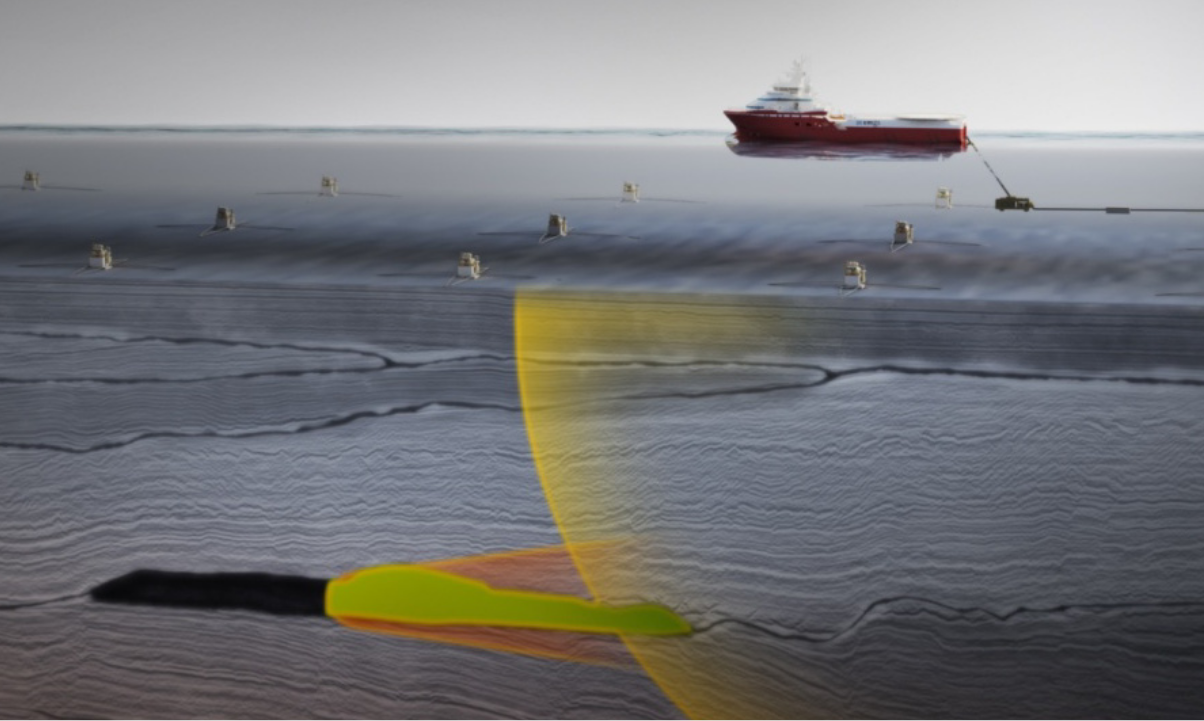
\includegraphics[scale=0.25]{theory/10000000000004B4000002D101BC1A4D.png}
	\caption{задача морской геоэлектрики}
	\label{fig:theory:ship}
\end{figure}

\vspace{-0.7cm}

К отличительным особенностям задач морской геоэлектрики относится низкая частота источника электромагнитного поля (0.25-100~Гц)~\citep{gabrielsen} и, как следствие, большой размер области моделирования. Кроме того, морское дно имеет сложный рельеф, а электропроводность морской воды может изменяться в зависимости от глубины~\citep{shurina}. Это вызвано различной соленостью и температурой разных слоев морской воды, эти свойства, кроме того, могут меняться от внешних факторов, таких как сезон, погодные условия или интенсивность таяния льдов.

Геометрические размеры локального источника возбуждения электромагнитного поля составляют несколько сотен метров, тогда как размеры области моделирования составляют 6000~м и более. Это приводит к необходимости применения специальных методов для сокращения расчетной области. Для этого нередко практикуется отказ от расчетов в области с воздухом и, вместо этого, задание на границе раздела сред воздух-вода условий непротекания. Однако такой подход не позволяет правильно учесть физические процессы, протекающие в воздухе~\citep{anderson}.
%TODO сослаться на НТИ-2015 еще!
Другим подходом является выделение из области некоторой подобласти меньшего размера и задание на ее границах специальных поглощающих условий. К таким условиям относятся Absorbing Boundary Conditions (ABC)~\citep{mur}, предложенные G.~Mur в 1981 году, а также Perfectly Matched Layer (PML)~\citep{berenger, wiik_dehoop_ursin}, который предложил J.P.~Berenger в 1994 году. PML-слой учитывается в вариационной формулировке как подобласть со специальными коэффициентами. 

В настоящее время для решения задач морской геоэлектрики наиболее широко используется векторный метод конечных элементов (ВМКЭ). Этот метод подробно освещен в работах \citep{balandin, monk}.

Целью работы является решение трехмерной прямой задачи морской геоэлектрики векторным методом конечных элементов. Для достижения поставленной цели были сформулированы следующие задачи:
\begin{enumerate}
	\item Исследование влияния слоя воздуха при различной глубине источника электромагнитного возмущения.
	\item Исследование целесообразности применения PML-слоя для ограничения области моделирования в задачах морской геоэлектрики на низких частотах.
	\item Исследование поведения электромагнитного поля при различном расположении источника поля и искомого объекта друг относительно друга.
\end{enumerate}

%TODO Написать про структуру работы, упомянуть все конференции
{\color{red}\textbf{Написать про структуру работы, упомянуть все конференции}}


\clearpage
\chapter{Тест тест тест}
\section{Математическая модель}
\subsection{Уравнения Максвелла и Гельмгольца}
Электромагнитное поле описывается системой уравнений Максвелла~\citep{epov}:
\begin{equation}
	\nabla \times \mathbf{E} = - \frac{ \partial \mathbf{B} }{ \partial t } \text{~~--~закон Фарадея}, \label{eq:maxwell:faradey}
\end{equation}
\begin{equation}
	\nabla \times \mathbf{H} = \frac{ \partial \mathbf{D} }{ \partial t } + \sigma \mathbf{E} + \mathbf{J} \text{~~--~закон Ампера}, \label{eq:maxwell:amper}
\end{equation}
\begin{equation*}
	\nabla \cdot \mathbf{B} = 0 \text{~~--~закон Гаусса для магнитной индукции}, \label{eq:maxwell:gauss_magn}
\end{equation*}
\begin{equation*}
	\nabla \cdot \mathbf{D} = \rho \text{~~--~закон Гаусса для электрической индукции}, \label{eq:maxwell:gauss_elect}
\end{equation*}
где $\mathbf{E}$~--~напряженность электрического поля~(В/м), $\mathbf{H}$~--~напряженность магнитного поля~(А/м), $\mathbf{B}=\mu \mathbf{H}$~--~магнитная индукция~(Тл), $\mathbf{D}=\varepsilon \mathbf{E}$~--~электрическая индукция~(Кл/м${}^2$), $\rho$~--~плотность электрических зарядов~(Кл/м${}^3$), $\sigma$~--~электрическая проводимость~(См/м), $\varepsilon = \varepsilon_r \varepsilon_0$~--~диэлектрическая проницаемость~(Ф/м), $\varepsilon_r$~--~относительная диэлектрическая проницаемость, $\varepsilon_0 = 8.85 \cdot 10^{-12}$~Ф/м~--~диэлектрическая проницаемость вакуума, $\mu = \mu_r \mu_0$~--~магнитная проницаемость~(Гн/м), $\mu_r$~--~относительная магнитная проницаемость, $\mu_0 = 4 \pi \cdot 10^{-7}$~Гн/м~--~магнитная проницаемость вакуума, $\mathbf{J}$~--~плотность стороннего электрического тока~(А/м${}^2$).

На границе $\Gamma = \Omega^j \cap \Omega^k$ между материалами $j$ и $k$ с различными электрофизическими свойствами должны быть выполнены следующие условия:
\begin{equation}
	\Jmp{ \mathbf{E} \times \mathbf{n} }_{\Gamma} = 0 \text{~~--~тангенциальная компонента $\mathbf{E}$ непрерывна}, \label{eq:maxwell:tangent_E}
\end{equation}
\begin{equation*}
	\Jmp{ \mathbf{B} \cdot \mathbf{n} }_{\Gamma} = 0 \text{~~--~нормальная компонента $\mathbf{B}$ непрерывна}, \label{eq:maxwell:normal_B}
\end{equation*}
\begin{equation*}
	\Jmp{ \mathbf{H} \times \mathbf{n} }_{\Gamma} = \mathbf{J}_{\Gamma} \text{~~--~тангенциальная компонента $\mathbf{H}$ разрывна}, \label{eq:maxwell:tangent_H}
\end{equation*}
\begin{equation}
	\Jmp{ \mathbf{D} \cdot \mathbf{n} }_{\Gamma} = \rho_{\Gamma} \text{~~--~нормальная компонента $\mathbf{D}$ разрывна}. \label{eq:maxwell:normal_D}
\end{equation}

При моделировании электрического поля в частотной области будем полагать, что $\mathbf{E}$ и $\mathbf{J}$ будут зависеть от времени по гармоническому закону:
\begin{equation*}
	\mathbf{E}(t) = \mathbf{E} e^{i \omega t} , \text{~~~~~} \mathbf{J}(t) = \mathbf{J} e^{i \omega t} .
\end{equation*}
Используя такое представление, получим из~(\ref{eq:maxwell:faradey}) и~(\ref{eq:maxwell:amper}):
\begin{equation}
	\nabla \times \mathbf{E} = - i \omega \mathbf{B} , \label{eq:form_5}
\end{equation}
\begin{equation}
	\nabla \times \mathbf{H} = i \omega \mathbf{D} + \sigma \mathbf{E} + \mathbf{J} . \label{eq:form_6}
\end{equation}
Выполним следующие преобразования над (\ref{eq:form_5}):
\begin{equation*}
	\nabla \times \mathbf{E} = - i \omega \mu \mathbf{H} ,
\end{equation*}
\begin{equation*}
	\mu^{-1} \nabla \times \mathbf{E} = - i \omega \mathbf{H} ,
\end{equation*}
\begin{equation}
	\nabla \times ( \mu^{-1} \nabla \times \mathbf{E} ) = - i \omega \nabla \times \mathbf{H} . \label{eq:form_9}
\end{equation}
Подставим в (\ref{eq:form_9}) (\ref{eq:form_6}):\nopagebreak
\begin{equation*}
	\nabla \times ( \mu^{-1} \nabla \times \mathbf{E} ) = - i \omega ( i \omega \varepsilon \mathbf{E} + \sigma \mathbf{E} + \mathbf{J} ) ,
\end{equation*}
\begin{equation*}
	\nabla \times ( \mu^{-1} \nabla \times \mathbf{E} ) = \omega^{2} \varepsilon \mathbf{E} - i \omega \sigma \mathbf{E} - i \omega \mathbf{J} ,
\end{equation*}
\begin{equation}
	\nabla \times ( \mu^{-1} \nabla \times \mathbf{E} ) + k^{2} \mathbf{E} = - i \omega \mathbf{J} , \label{eq:helmholtz}
\end{equation}
где $k^{2} = i \omega \sigma - \omega^{2} \varepsilon$. Уравнение~(\ref{eq:helmholtz}) называется уравнением Гельмгольца.

Краевые условия для уравнения (\ref{eq:helmholtz}) можно записать следующим образом:
\begin{equation}
	\left. \mathbf{E} \times \mathbf{n} \right | _{ S_1 } = {\mathbf{E}} ^g , \label{eq:bound1}
\end{equation}
\begin{equation}
	\left. \sigma \mathbf{E} \cdot \mathbf{n} \right | _{ S_2 } = 0 . \label{eq:bound2}
\end{equation}
В случае удаленных границ (\ref{eq:bound1}) принимает вид условия <<большого бака>>:
\begin{equation}
	\left. \mathbf{E} \times \mathbf{n} \right | _{ S_1 } = 0 . \label{eq:bound1_zero}
\end{equation}
Источником электромагнитного возмущения будет выступать замкнутая токовая петля.

Подействуем оператором $\nabla \cdot$ на уравнение~(\ref{eq:maxwell:amper}):
\begin{equation*}
	\nabla \cdot ( \nabla \times \mathbf{H} ) = \nabla \cdot ( \frac{\partial \mathbf{D}}{\partial t} + \sigma \mathbf{E} + \mathbf{J} ) .
\end{equation*}
Так как $\nabla \cdot ( \nabla \times \mathbf{H} ) = 0$, $\nabla \cdot \frac{\partial \mathbf{D}}{\partial t} = \nabla \cdot \frac{\partial \varepsilon \mathbf{E}}{\partial t} = \nabla \cdot (i \omega \varepsilon \mathbf{E})$ и, так как для замкнутой петли с током выполняется $\nabla \cdot \mathbf{J} = 0$, получим закон сохранения заряда:
\begin{equation}
	\nabla \cdot ( \sigma + i \omega \varepsilon ) \mathbf{E} = 0 . \label{eq:charge}
\end{equation}

% =============================================================================

\subsection{Вариационная постановка}
Введем следующие пространства~\citep{balandin,monk}:
\begin{equation*}
	\mathbb{H} ( \mathrm{rot}\,, \Omega ) = \lbrace \mathbf{v} \in [\mathbb{L}^{2}(\Omega)]^{3} : \nabla \times \mathbf{v} \in [\mathbb{L}^{2}(\Omega)]^{3} \rbrace , \label{eq:H_rot}
\end{equation*}
\begin{equation*}
	\mathbb{H}_{0}( \mathrm{rot}\,, \Omega ) = \lbrace \mathbf{v} \in \mathbb{H}(\mathrm{rot}\,, \Omega) : \left. \mathbf{v} \times \mathbf{n} \right|_{\partial \Omega} = 0  \rbrace . \label{eq:H0_rot}
\end{equation*}
Эти пространства имеют скалярное произведение и норму:
\begin{equation*}
	( \mathbf{u}, \mathbf{v} ) = \int\limits_{\Omega} \mathbf{u} \cdot \mathbf{v}^{*} \,d\Omega ,
\end{equation*}
\begin{equation*}
	\left \| \mathbf{u} \right \| ^{2} = \int\limits_{\Omega} \mathbf{u} \cdot \mathbf{u}^{*} \,d\Omega + \int\limits_{\Omega} ( \nabla \times \mathbf{u} ) \cdot ( \nabla \times \mathbf{u}^{*} ) \,d\Omega ,
\end{equation*}
где индекс $*$ обозначает комплексное сопряжение.

Скалярно умножим (\ref{eq:helmholtz}) на некоторую пробную функцию $\mathbf{v} \in \mathbb{H}_{0}( \mathrm{rot}\,, \Omega )$:
\begin{equation*}
	(\nabla \times ( \mu^{-1} \nabla \times \mathbf{E} ), \mathbf{v}) + (k^{2} \mathbf{E} , \mathbf{v}) = - (i \omega \mathbf{J} , \mathbf{v}) ,
\end{equation*}
\begin{equation*}
	\int\limits_\Omega \nabla \times ( \mu^{-1} \nabla \times \mathbf{E} ) \cdot \mathbf{v}^{*} \,d\Omega + \int\limits_\Omega k^{2} \mathbf{E} \cdot \mathbf{v}^{*} \,d\Omega = - \int\limits_\Omega i \omega \mathbf{J} \cdot \mathbf{v}^{*} \,d\Omega .
\end{equation*}
Воспользовавшись первой векторной формулой Грина (\ref{eq:green}):
\begin{equation}
	\int\limits_D \nabla \times \mathbf{u} \cdot \mathbf{v}^{*} \,dV = \int\limits_D \mathbf{u} \cdot ( \nabla \times \mathbf{v}^{*} ) \,dV + \int\limits_{\partial D} (\mathbf{n} \times \mathbf{u}) \cdot \mathbf{v}^{*} \,dS , \label{eq:green}
\end{equation}
получим:
\begin{equation*}
	\begin{array}{c} { \displaystyle
		\int\limits_\Omega \mu^{-1} \nabla \times \mathbf{E} \cdot \nabla \times \mathbf{v}^{*} \,d\Omega
		+ \int\limits_{\partial \Omega} \mathbf{n} \times (\mu^{-1} \nabla \times \mathbf{E}) \cdot \mathbf{v}^{*} \,dS
		+
	} \\ { \displaystyle
		+ \int\limits_\Omega k^{2} \mathbf{E} \cdot \mathbf{v}^{*} \,d\Omega
		=  - \int\limits_\Omega i \omega \mathbf{J} \cdot \mathbf{v}^{*} \,d\Omega
		.
	} \end{array}
\end{equation*}
Применим тождества $(\mathbf{a} \times \mathbf{b}) \cdot \mathbf{c} = - (\mathbf{a} \times \mathbf{c}) \cdot \mathbf{b}$ и $\mathbf{a} \times \mathbf{b} = - \mathbf{b} \times \mathbf{a}$:
\begin{equation}
	\begin{array}{c} { \displaystyle
		\int\limits_\Omega \mu^{-1} \nabla \times \mathbf{E} \cdot \nabla \times \mathbf{v}^{*} \,d\Omega
		+ \int\limits_\Omega k^{2} \mathbf{E} \cdot \mathbf{v}^{*} \,d\Omega
		=
	} \\ { \displaystyle
		= - \int\limits_\Omega i \omega \mathbf{J} \cdot \mathbf{v}^{*} \,d\Omega
		- \int\limits_{\partial \Omega} \mathbf{v}^{*} \times \mathbf{n} \cdot (\mu^{-1} \nabla \times \mathbf{E}) \,dS
	.
	} \end{array}
	\label{eq:form_23}
\end{equation}
Так как $\mathbf{v} \in \mathbb{H}_{0}( \mathrm{rot}\,, \Omega )$, то из свойств пространства $\mathbb{H}_{0}( \mathrm{rot}\,, \Omega )$ второй интеграл в правой части равен нулю, тогда уравнение (\ref{eq:form_23}) примет вид:
\begin{equation}
	\int\limits_\Omega \mu^{-1} \nabla \times \mathbf{E} \cdot \nabla \times \mathbf{v}^{*} \,d\Omega + \int\limits_\Omega k^{2} \mathbf{E} \cdot \mathbf{v}^{*} \,d\Omega = - \int\limits_\Omega i \omega \mathbf{J} \cdot \mathbf{v}^{*} \,d\Omega . \label{eq:weak}
\end{equation}

В результате векторная вариационная постановка имеет вид: \textbf{\textit{Найти $\mathbf{E} \in \mathbb{H}_{0}( \mathrm{rot}\,, \Omega )$, такое что $\forall \mathbf{v} \in \mathbb{H}_{0}( \mathrm{rot}\,, \Omega )$ будет выполнено}} (\ref{eq:weak}).

Рассмотрим еще пару пространств~\citep{monk}
\begin{equation*}
	\mathbb{H}( \mathrm{grad}\,, \Omega ) = \lbrace \varphi \in \mathbb{L}^{2}(\Omega) : \nabla \varphi \in [ \mathbb{L}^{2}(\Omega) ]^{3} \rbrace , \label{eq:H_grad}
\end{equation*}
\begin{equation*}
	\mathbb{H}_{0}( \mathrm{grad}\,, \Omega ) = \lbrace \varphi \in \mathbb{H}( \mathrm{grad}\,, \Omega ) : \left. \varphi \right | _{\partial \Omega} = 0 \rbrace . \label{eq:H0_grad}
\end{equation*}
В соответствии с комплексом Де Рама (De Rham)~\citep{schwarzbach}
\begin{equation}
	\mathbb{H}( \mathrm{grad}\,, \Omega ) \xrightarrow[]{\nabla} \mathbb{H}( \mathrm{rot}\,, \Omega ) \xrightarrow[]{\nabla \times} \mathbb{H}( \mathrm{div}\,, \Omega ) \xrightarrow[]{\nabla \cdot} \mathbb{L}^{2}(\Omega) , \label{eq:derham}
\end{equation}
будет иметь место вложение $\nabla \varphi \in \mathbb{H}_{0}( \mathrm{rot}\,, \Omega )$, $\forall \varphi \in \mathbb{H}_{0}( \mathrm{grad}\,, \Omega )$. Возьмем $\mathbf{v} = \nabla \varphi$, тогда (\ref{eq:weak}) примет вид:
\begin{equation*}
	\int\limits_\Omega \mu^{-1} \nabla \times \mathbf{E} \cdot \nabla \times (\nabla \varphi)^{*} \,d\Omega + \int\limits_\Omega k^{2} \mathbf{E} \cdot (\nabla \varphi)^{*} \,d\Omega = - \int\limits_\Omega i \omega \mathbf{J} \cdot (\nabla \varphi)^{*} \,d\Omega .
\end{equation*}
Использовав свойство дивергенции $\nabla \cdot (\varphi \mathbf{F}) = \nabla \varphi \cdot \mathbf{F} + \varphi \nabla \cdot \mathbf{F}$ и применив формулу Ос\-т\-ро\-г\-ра\-д\-с\-ко\-го-Гаусса~(\ref{eq:divergence_theorem})
\begin{equation}
	\int\limits_{D} \nabla \cdot \mathbf{F} \,dV = \int\limits_{\partial D} \mathbf{F} \cdot \mathbf{n} \,dS ,
	\label{eq:divergence_theorem}
\end{equation}
получим:
\begin{equation*}
	\int\limits_\Omega \mu^{-1} \nabla \times \mathbf{E} \cdot \nabla \times (\nabla \varphi)^{*} \,d\Omega + \int\limits_\Omega k^{2}\, \mathbf{E} \cdot (\nabla \varphi)^{*} \,d\Omega = - \int\limits_\Omega i \omega \varphi^{*} \nabla \cdot \mathbf{J} \,d\Omega - \int\limits_{\partial \Omega} i \omega \varphi^{*} \mathbf{J} \cdot \mathbf{n} \,d S .
\end{equation*}
Поскольку $\nabla \times (\nabla \varphi) = 0$, $\nabla \cdot \mathbf{J} = 0$ и $\left. \varphi \right | _{\partial \Omega} = 0$, в левой части останется только один интеграл:
\begin{equation*}
	\int\limits_\Omega k^{2}\, \mathbf{E} \cdot (\nabla \varphi)^{*} \,d\Omega = 0 .
\end{equation*}
Снова применим свойство дивергенции $\nabla \cdot (\varphi \mathbf{F}) = \nabla \varphi \cdot \mathbf{F} + \varphi \nabla \cdot \mathbf{F}$:
\begin{equation*}
	\int\limits_\Omega \nabla \cdot ( k^{2}\, \mathbf{E} \varphi^{*} ) \,d\Omega
	- \int\limits_\Omega \varphi^{*} \nabla \cdot ( k^{2}\, \mathbf{E} ) \,d\Omega = 0 ,
\end{equation*}
после чего применим формулу Остроградского-Гаусса~(\ref{eq:divergence_theorem}):
\begin{equation*}
	\int\limits_{\partial \Omega} ( k^{2}\, \mathbf{E} \varphi^{*} ) \cdot \mathbf{n} \,d S
	- \int\limits_\Omega \varphi^{*} \nabla \cdot ( k^{2}\, \mathbf{E} ) \,d\Omega = 0 .
\end{equation*}
С учетом условия $\left. \varphi \right | _{\partial \Omega} = 0$, получим:
\begin{equation*}
	\int\limits_\Omega \varphi^{*} \nabla \cdot ( k^{2}\, \mathbf{E} ) \,d\Omega = 0 ,
\end{equation*}
следовательно, решение вариационной задачи (\ref{eq:weak}) удовлетворяет закону сохранения заряда (\ref{eq:charge}) в слабом смысле.

% =============================================================================

\subsection{Вариационная постановка с учетом PML-слоя}
Для ограничения расчетной области вводится PML-слой ${\Omega^{PML}}$ согласно рисунку \ref{fig:theory:area_3layers_PML}, который определяется модифицированными координатами $\tilde{x}$, $\tilde{y}$, $\tilde{z}$, полученными следующей заменой координат ~\citep{wiik_dehoop_ursin}:
\begin{equation*}
	\tilde{x} = \int\limits_0^x s_x (t) \,dt ,
	\text{~~~~~}
	\tilde{y} = \int\limits_0^y s_y (t) \,dt ,
	\text{~~~~~}
	\tilde{z} = \int\limits_0^z s_z (t) \,dt ,
\end{equation*}
где $s_j(\tau) = 1$ вне PML-слоя, а внутри него может быть задано в виде:
\begin{equation}
	s_j(\tau) = 1 + \chi \left( \frac{d(\tau)}{\delta} \right)^m , \text{~~} m \geq 1 ,
	\label{eq:pml_s}
\end{equation}
где $d(\tau)$ -- расстояние в $j$-м направлении от внутренней границы PML-слоя, $\delta$ -- толщина PML-слоя, $\chi$ -- некоторое комплексное число, причем $\Re(\chi) \ge 0$, $\Im(\chi) \ge 0$. Оператор $\nabla$ в новых координатах будет иметь вид:
\begin{equation*}
	\tilde{\nabla} = \left[ \frac{1}{s_x} \frac{\partial}{\partial x} \,, \frac{1}{s_y} \frac{\partial}{\partial y} \,, \frac{1}{s_z} \frac{\partial}{\partial z} \right] .
\end{equation*}

\begin{figure}[H]
	\centering
	% trim=left bottom right top
	\subfloat[][]{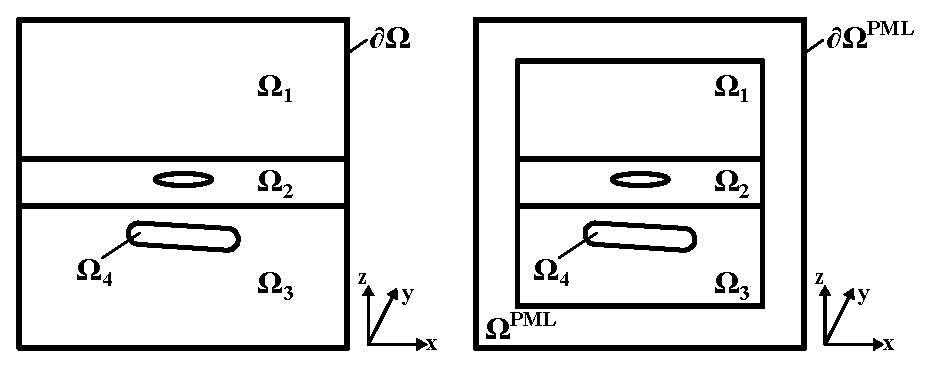
\includegraphics[trim=0mm 0mm 79.0mm 0mm,clip,scale=1]{theory/area_3layers_PML.eps}\label{fig:theory:area_3layers_PML_a}}
	\subfloat[][]{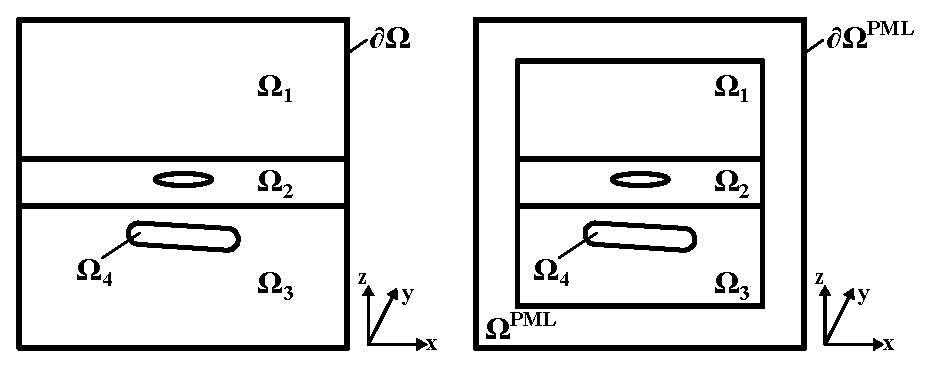
\includegraphics[trim=77.0mm 0mm 0mm 0mm,clip,scale=1]{theory/area_3layers_PML.eps}\label{fig:theory:area_3layers_PML_b}}
	\caption{расчетные области: (а) без PML-слоя и (б) с PML-слоем}
	\label{fig:theory:area_3layers_PML}
\end{figure}

После такой замены, внутри PML-слоя уравнение Гельмгольца (\ref{eq:helmholtz}) будет иметь вид (\ref{eq:helmholtz_pml})
\begin{equation}
	\tilde{\nabla} \times ( \mu^{-1} \tilde{\nabla} \times \tilde{\mathbf{E}} ) + k^{2} \tilde{\mathbf{E}} = 0 , \label{eq:helmholtz_pml}
\end{equation}
что приведет к преобразованию уравнения (\ref{eq:weak}) к виду (\ref{eq:weak_pml}):
\begin{equation}
	\int\limits_{{\Omega^{PML}}} \mu^{-1} \tilde{\nabla} \times \tilde{\mathbf{E}} \cdot \tilde{\nabla} \times \mathbf{v}^{*} \,d{\Omega^{PML}} + \int\limits_{{\Omega^{PML}}} k^{2} \tilde{\mathbf{E}} \cdot \mathbf{v}^{*} \,d{\Omega^{PML}} = 0 . \label{eq:weak_pml}
\end{equation}

В результате, если обозначить $\widehat{\Omega} = \Omega \setminus {\Omega^{PML}}$, то векторная вариационная постановка с учетом PML-слоя примет вид: \textbf{\textit{Найти $\mathbf{E} \in \mathbb{H}_{0}( \mathrm{rot}\,, \widehat{\Omega} )$ и  $\tilde{\mathbf{E}} \in \mathbb{H}_{0}( \mathrm{rot}\,, {\Omega^{PML}} )$, такие что $\forall \mathbf{v} \in \mathbb{H}_{0}( \mathrm{rot}\,, \widehat{\Omega} )$ и $\forall \tilde{\mathbf{v}} \in \mathbb{H}_{0}( \mathrm{rot}\,, {\Omega^{PML}} )$ будет выполнено}}:
\begin{equation*}
	\begin{cases}
		\displaystyle
		\int\limits_{\widehat{\Omega}} \mu^{-1} \nabla \times \mathbf{E} \cdot \nabla \times \mathbf{v}^{*} \,d\widehat{\Omega} + \int\limits_{\widehat{\Omega}} k^{2} \mathbf{E} \cdot \mathbf{v}^{*} \,d\widehat{\Omega} = - \int\limits_{\widehat{\Omega}} i \omega \mathbf{J} \cdot \mathbf{v}^{*} \,d\widehat{\Omega} \\
		\displaystyle
		\int\limits_{{\Omega^{PML}}} \mu^{-1} \tilde{\nabla} \times \tilde{\mathbf{E}} \cdot \tilde{\nabla} \times \tilde{\mathbf{v}}^{*} \,d{\Omega^{PML}} + \int\limits_{{\Omega^{PML}}} k^{2} \tilde{\mathbf{E}} \cdot \tilde{\mathbf{v}}^{*} \,d{\Omega^{PML}} = 0 . \\
	\end{cases}
\end{equation*}

% =============================================================================

\subsection{Дискретная вариационная постановка}
Разобьем область $\Omega$ на $m$ непересекающихся элементов:
\begin{equation*}
	\Omega = \bigcup\limits_{k=1}^{m} \Omega_k , \text{~~} \forall i \neq j , \text{~~} \Omega_i \cap \Omega_j = \varnothing .
\end{equation*}

Введем конечномерные подпространства:
\begin{equation*}
	\mathbb{H}_{0}^h( \mathrm{rot}\,, \Omega ) \subset \mathbb{H}_{0}( \mathrm{rot}\,, \Omega ) , \text{~~}
	\mathbb{H}_{0}^h( \mathrm{grad}\,, \Omega ) \subset \mathbb{H}_{0}( \mathrm{grad}\,, \Omega ) .
\end{equation*}
Для дискретных подпространств $\mathbb{H}_{0}^h( \mathrm{rot}\,, \Omega )$ и $\mathbb{H}_{0}^h( \mathrm{grad}\,, \Omega )$ комплекс Де Рама~(\ref{eq:derham}) также будет верен, следовательно закон сохранения заряда~(\ref{eq:charge}) будет также выполнен в слабом смысле.

Пространство $\mathbb{H}_{0}^h( \mathrm{rot}\,, \Omega )$ является прямой суммой подпространств~\citep{hiptmair}
\begin{equation*}
	\mathbb{H}_{0}^h( \mathrm{rot}\,, \Omega ) = \mathbb{N}_{0}^h( \mathrm{rot}\,, \Omega ) \oplus (\mathbb{N}_{0}^h( \mathrm{rot}\,, \Omega ))^{\bot} ,
\end{equation*}
где $\mathbb{N}_{0}^h( \mathrm{rot}\,, \Omega )$ -- ядро rot-оператора, $(\mathbb{N}_{0}^h( \mathrm{rot}\,, \Omega ))^{\bot}$ -- его ортогональное дополнение. Для выполнения условий непрерывности (\ref{eq:maxwell:tangent_E})-(\ref{eq:maxwell:normal_D}) необходимо использовать полный базис (базис II типа) \citep{webb1993,webb1999,nedelec1980,nedelec1986}, состоящий из роторных базисных функций, принадлежащих пространству $(\mathbb{N}_{0}^h( \mathrm{rot}\,, \Omega ))^{\bot}$ и обеспечивающих непрерывность тангенциальных компонент электрического поля $\mathbf{E}$ (\ref{eq:maxwell:tangent_E}), и градиентных базисных функций из пространства $\mathbb{N}_{0}^h( \mathrm{rot}\,, \Omega )$, отвечающих за скачок нормальной компоненты электрического поля $\mathbf{E}$~(\ref{eq:maxwell:normal_D}) и выполнения закона сохранения заряда~(\ref{eq:charge}).

Представим векторнозначную функцию $\mathbf{E}^h$ в виде разложения по базису \linebreak $\boldsymbol{\psi}_j \in \mathbb{H}_{0}^h( \mathrm{rot}\,, \Omega )$:
\begin{equation*}
	\mathbf{E}^h = \sum\limits_{j = 1}^n q_j \boldsymbol{\psi}_j .
\end{equation*}
В качестве тестовой функции выберем базисную функцию $\boldsymbol{\psi}_i \in \mathbb{H}_{0}^h( \mathrm{rot}\,, \Omega )$, тогда конечноэлементная аппроксимация вариационного уравнения (\ref{eq:weak}) примет вид:
\begin{equation}
	\begin{array}{c} { \displaystyle
		\sum\limits_{j = 1}^n \left( \int\limits_\Omega \mu^{-1} \nabla \times \boldsymbol{\psi}_j \cdot \nabla \times \boldsymbol{\psi}_i \,d\Omega + \int\limits_\Omega k^{2} \boldsymbol{\psi}_j \cdot \boldsymbol{\psi}_i \,d\Omega \right) q_j =
	} \\ { \displaystyle
		=  - \int\limits_\Omega i \omega \mathbf{J} \cdot \boldsymbol{\psi}_i \,d\Omega .
	} \end{array}
	\label{eq:weak_discr}
\end{equation}

В матрично-векторной форме (\ref{eq:weak_discr}) можно представить следующим образом:
\begin{equation}
	( G + M )q = F , \label{eq:form_29}
\end{equation}
где:
\begin{equation*}
	G_{ i,j } = \int\limits_{\Omega_k} \mu^{-1} \nabla \times \mathbf{w}_i \cdot \nabla \times \mathbf{w}_j \,d\Omega_k , \text{~~~}
	M_{ i,j } = \int\limits_{\Omega_k} k^2 \mathbf{w}_i \cdot \mathbf{w}_j \,d\Omega_k . \label{eq:local_matrixes}
\end{equation*}
% Система линейных алгебраических уравнений (СЛАУ) (\ref{eq:slae}) решается специальным двухуровневым методом~\citep{nechaev}.

% =============================================================================

\subsection{Тетраэдральные конечные элементы}

В качестве конечных элементов для представления расчетной области, будем пользоваться тетраэдрами. На тетраэдральном конечном элементе определим $\mathcal{L}$-ко\-ор\-ди\-на\-ты, называемые также барицентрическими координатами~\citep{soloveychick}. Введем нумерацию вершин и ребер, показанную на рисунке \ref{fig:theory:tetrahedron}:
\begin{figure}[H]
	\centering
	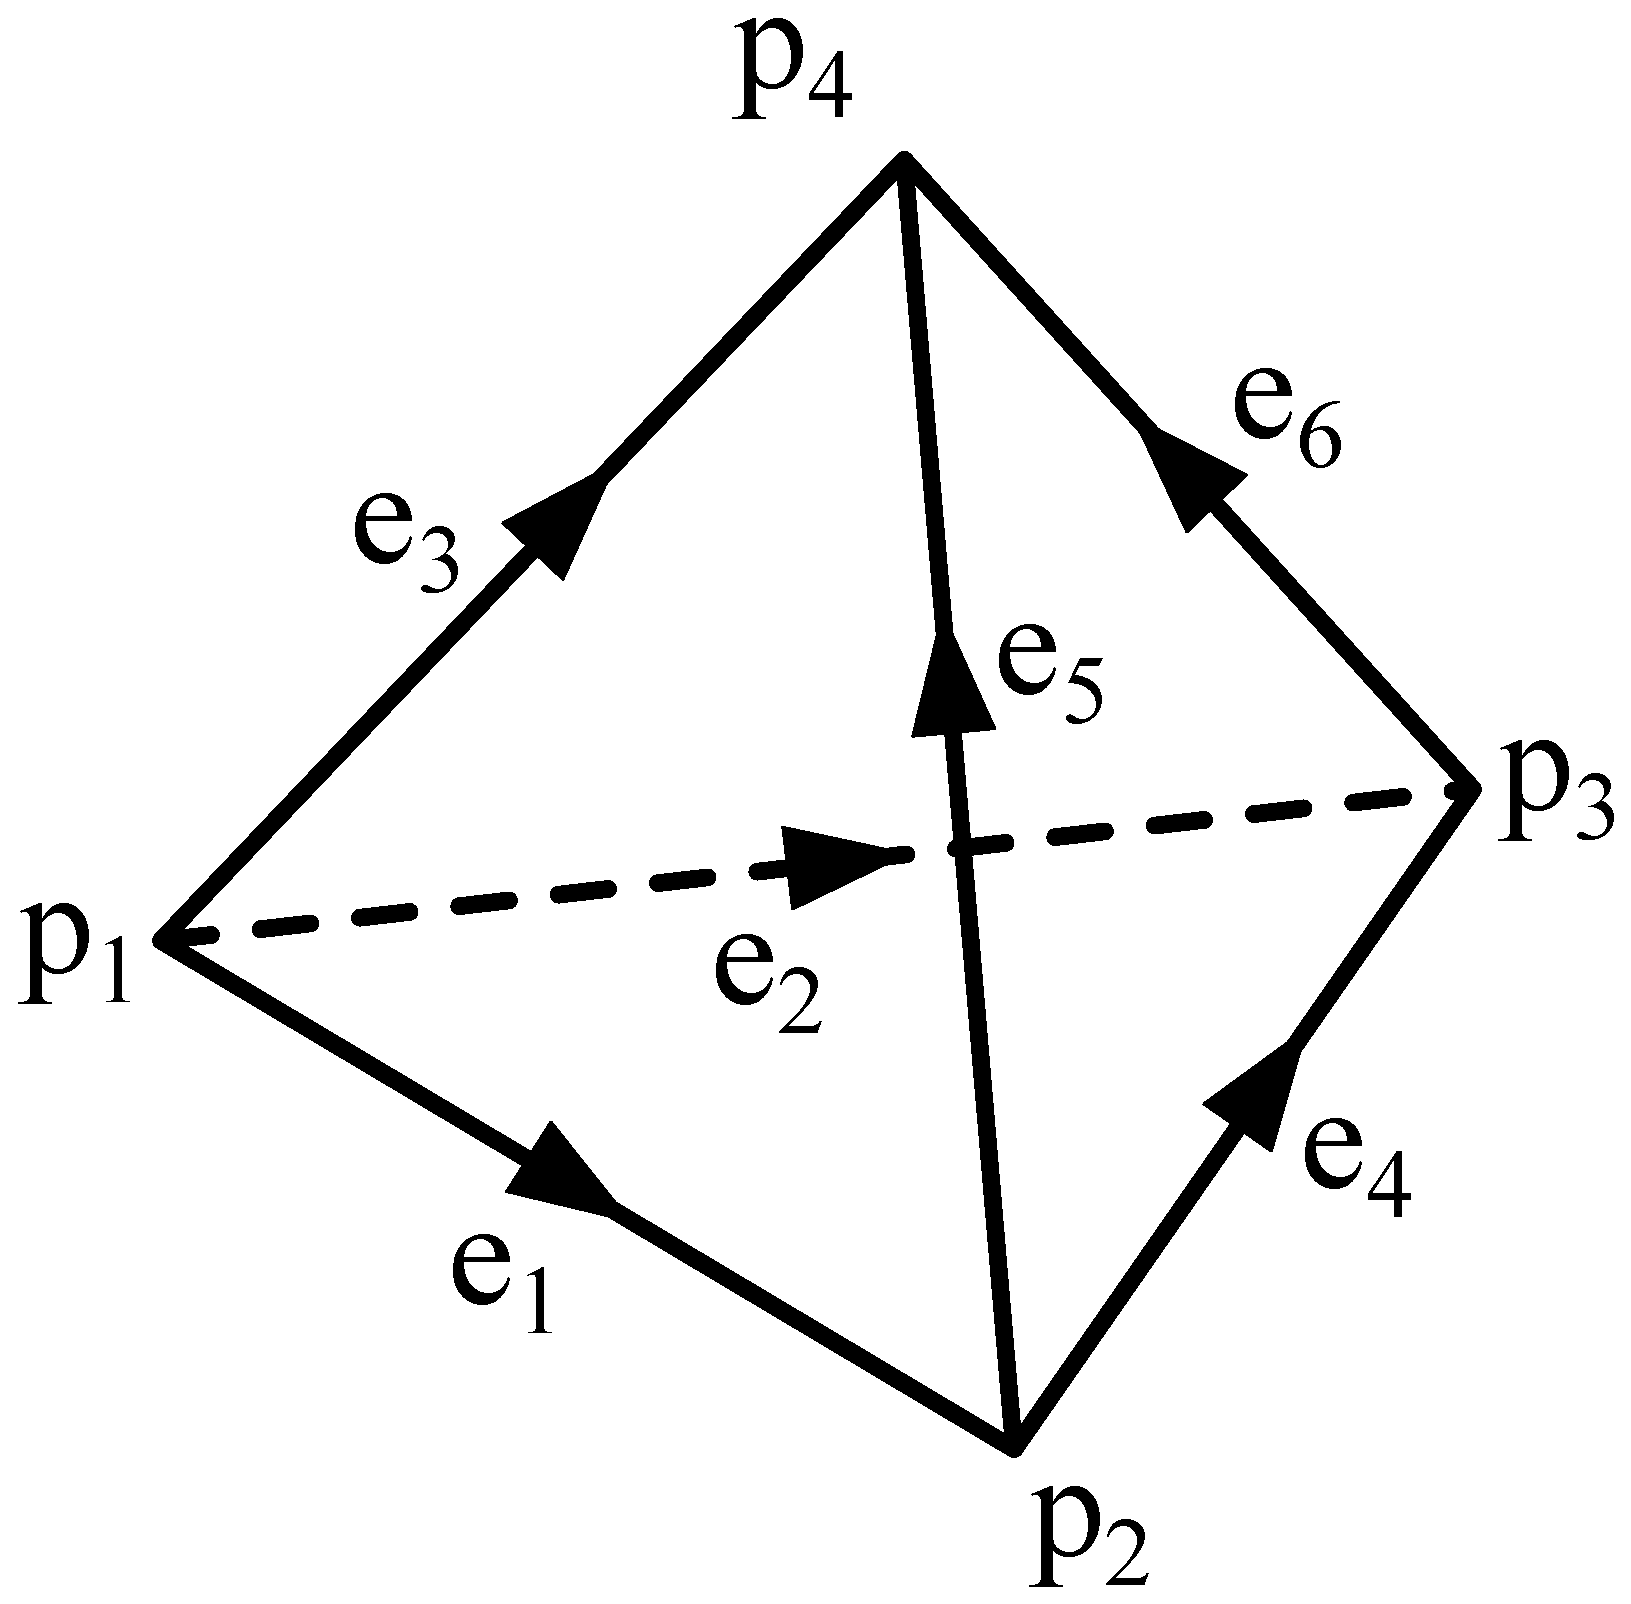
\includegraphics[scale=0.25]{theory/tetrahedron.eps}
	\caption{тетраэдральный конечный элемент}
	\label{fig:theory:tetrahedron}
\end{figure}

\noindent Под $\mathcal{L}$-координатами понимают функции следующего вида:
\begin{equation*}
	\mathcal{L}_i (x, y, z) = \alpha_{i, 1} x + \alpha_{i, 2} y + \alpha_{i, 3} z + \alpha_{i, 4} , \text{~~~} i = \overline{1..4} . \label{eq:tet:L}
\end{equation*}
Коэффициенты $\alpha_{i, j}$ могут быть определены по формуле (\ref{eq:tet:D1}):
\begin{equation}
	\left[
	\begin{matrix}
		\alpha_{1, 1} & \alpha_{1, 2} & \alpha_{1, 3} & \alpha_{1, 4} \\
		\alpha_{2, 1} & \alpha_{2, 2} & \alpha_{2, 3} & \alpha_{2, 4} \\
		\alpha_{3, 1} & \alpha_{3, 2} & \alpha_{3, 3} & \alpha_{3, 4} \\
		\alpha_{4, 1} & \alpha_{4, 2} & \alpha_{4, 3} & \alpha_{4, 4} \\
	\end{matrix}
	\right] = \left[
	\begin{matrix}
		{p_1}_x & {p_2}_x & {p_3}_x & {p_4}_x \\
		{p_1}_y & {p_2}_y & {p_3}_y & {p_4}_y \\
		{p_1}_z & {p_2}_z & {p_3}_z & {p_4}_z \\
		1 & 1 & 1 & 1 \\
	\end{matrix}
	\right]^{-1} = D^{-1} . \label{eq:tet:D1}
\end{equation}

Задав $\mathcal{L}$-координаты, можно определить на тетраэдре базисные функции. В отличие от узлового метода конечных элементов, в векторном методе конечных элементов базисные функции ассоциированы не с узлами, а с ребрами (edge), гранями (face) и объемами (volume)~\citep{nechaev, webb1999}. Так как будут использованы полные (II типа) базисы первого и второго порядков, то ограничимся рассмотрением только базисных функций, ассоциированных с ребрами и гранями.

Иерархический векторный базис Вебба второго порядка второго типа на тетраэдрах имеет вид~\citep{mikhajlova}:
\begin{equation*}
	\begin{matrix}
		\displaystyle
		\mathbf{w}_{i}^{1,\mathrm{I}} = \mathcal{L}_k \nabla \mathcal{L}_l - \mathcal{L}_l \nabla \mathcal{L}_k ;
		\scriptstyle
		\text{~~} i = 1, ..., 6 ; \text{~~} k, l = 1, ..., 4 ; \text{~~} k < l ,\\
		\displaystyle
		\mathbf{w}_{i}^{1,\mathrm{II}} = \mathcal{L}_k \nabla \mathcal{L}_l + \mathcal{L}_l \nabla \mathcal{L}_k ;
		\scriptstyle
		\text{~~} i = 7, ..., 12 ; \text{~~} k, l = 1, ..., 4 ; \text{~~} k < l ,\\
		\displaystyle
		\mathbf{w}_{i}^{2,\mathrm{I}} = \mathcal{L}_k \mathcal{L}_l \nabla \mathcal{L}_j + \mathcal{L}_j \mathcal{L}_l \nabla \mathcal{L}_k - 2 \mathcal{L}_j \mathcal{L}_k \nabla \mathcal{L}_l ;
		\scriptstyle
		\text{~~} i = 13, ..., 16 ; \text{~~} j, k, l = 1, ..., 4 ; \text{~~} j < k < l ,\\
		\displaystyle
		\mathbf{w}_{i}^{2,\mathrm{I}} = \mathcal{L}_k \mathcal{L}_l \nabla \mathcal{L}_j - 2 \mathcal{L}_j \mathcal{L}_l \nabla \mathcal{L}_k + \mathcal{L}_j \mathcal{L}_k \nabla \mathcal{L}_l ;
		\scriptstyle
		\text{~~} i = 17, ..., 20 ; \text{~~} j, k, l = 1, ..., 4 ; \text{~~} j < k < l ,\\
		\displaystyle
		\mathbf{w}_{i}^{2,\mathrm{II}} = \nabla ( \mathcal{L}_j \mathcal{L}_k \mathcal{L}_l ) ;
		\scriptstyle
		\text{~~} i = 21, ..., 24 ; \text{~~} j, k, l = 1, ..., 4 ; \text{~~} j < k < l ,\\
		\displaystyle
		\mathbf{w}_{i}^{2,\mathrm{II}} = \nabla ( \mathcal{L}_j \mathcal{L}_k ( \mathcal{L}_j - \mathcal{L}_k ) ) ;
		\scriptstyle
		\text{~~} i = 25, ..., 30 ; \text{~~} j, k = 1, ..., 4 ; \text{~~} j < k ,
	\end{matrix}
	\label{eq:basis}
\end{equation*}
где $\mathbf{w}_{1}^{1,\mathrm{I}}, ..., \mathbf{w}_{6}^{1,\mathrm{I}}$ -- базисные функции первого порядка первого типа, ассоциированные с ребрами, $\mathbf{w}_{7}^{1,\mathrm{II}}, ..., \mathbf{w}_{12}^{1,\mathrm{II}}$ -- базисные функции первого порядка второго типа, ассоциированные с ребрами, $\mathbf{w}_{13}^{2,\mathrm{I}}, ..., \mathbf{w}_{20}^{2,\mathrm{I}}$ -- базисные функции второго порядка первого типа, ассоциированные с гранями, $\mathbf{w}_{21}^{2,\mathrm{II}}, ..., \mathbf{w}_{30}^{2,\mathrm{II}}$ -- базисные функции второго порядка второго типа, ассоциированные с гранями (первые четыре) и ребрами. Так как этот базис иерархический, то для получения базиса меньшего порядка следует ограничиться меньшим количеством функций. Так, для базиса первого порядка второго  типа следует использовать функции $\mathbf{w}_{1}^{1,\mathrm{I}}, ..., \mathbf{w}_{12}^{1,\mathrm{II}}$.

Для вычисления интегралов в (\ref{eq:weak_discr}) воспользуемся кубатурной формулой численного интегрирования (формулой Гаусса)~\citep{misovskih}:
\begin{equation*}
	\int\limits_{\Omega_k} f(x, y, z) \,d\Omega_k = \sum\limits_{i = 1}^m f( x_i , y_i , z_i ) w_i ,
\end{equation*}
где $(x_i , y_i , z_i )$ -- точки Гаусса, $m$ -- число точек Гаусса, $w_i$ -- соответствующие веса. При работе с базисными функциями второго порядка нужно использовать формулы, которые бы обеспечивали восьмой порядок интегрирования~\citep{zhang_integration}. Для базисных функций первого порядка будет достаточно и меньших порядков интегрирования~\citep{tet_integration, misovskih}.

% =============================================================================

\subsection{Треугольные конечные элементы}

Границы области $\Omega$ являются двумерными и представляют собой треугольники. Для учета краевых условий (\ref{eq:bound1}) требуется построить разложение $\mathbf{E}^g$ по базису соответствующей границы в смысле МНК, для этого нужно решать СЛАУ вида
\begin{equation}
	M^{S_1} \tilde{q} = b^{S_1} ,
	\label{eq:bound_mnk}
\end{equation}
где $\displaystyle M^{S_1}_{i,j} = \int\limits_{S_1} \mathbf{w}_i \cdot \mathbf{w}_j \,d S_1$, $\displaystyle b^{S_1}_{i} = \int\limits_{S_1} \mathbf{E}^g \cdot \mathbf{w}_i \,d S_1$, $\mathbf{w}_i$ и $\mathbf{w}_j$ -- базисные функции на треугольниках.

Определим $\mathcal{L}$-координаты на треугольниках таким же образом, как и на тетраэдрах. Введем нумерацию вершин и ребер согласно рисунку \ref{fig:theory:triangle}:
\begin{figure}[H]
	\centering
	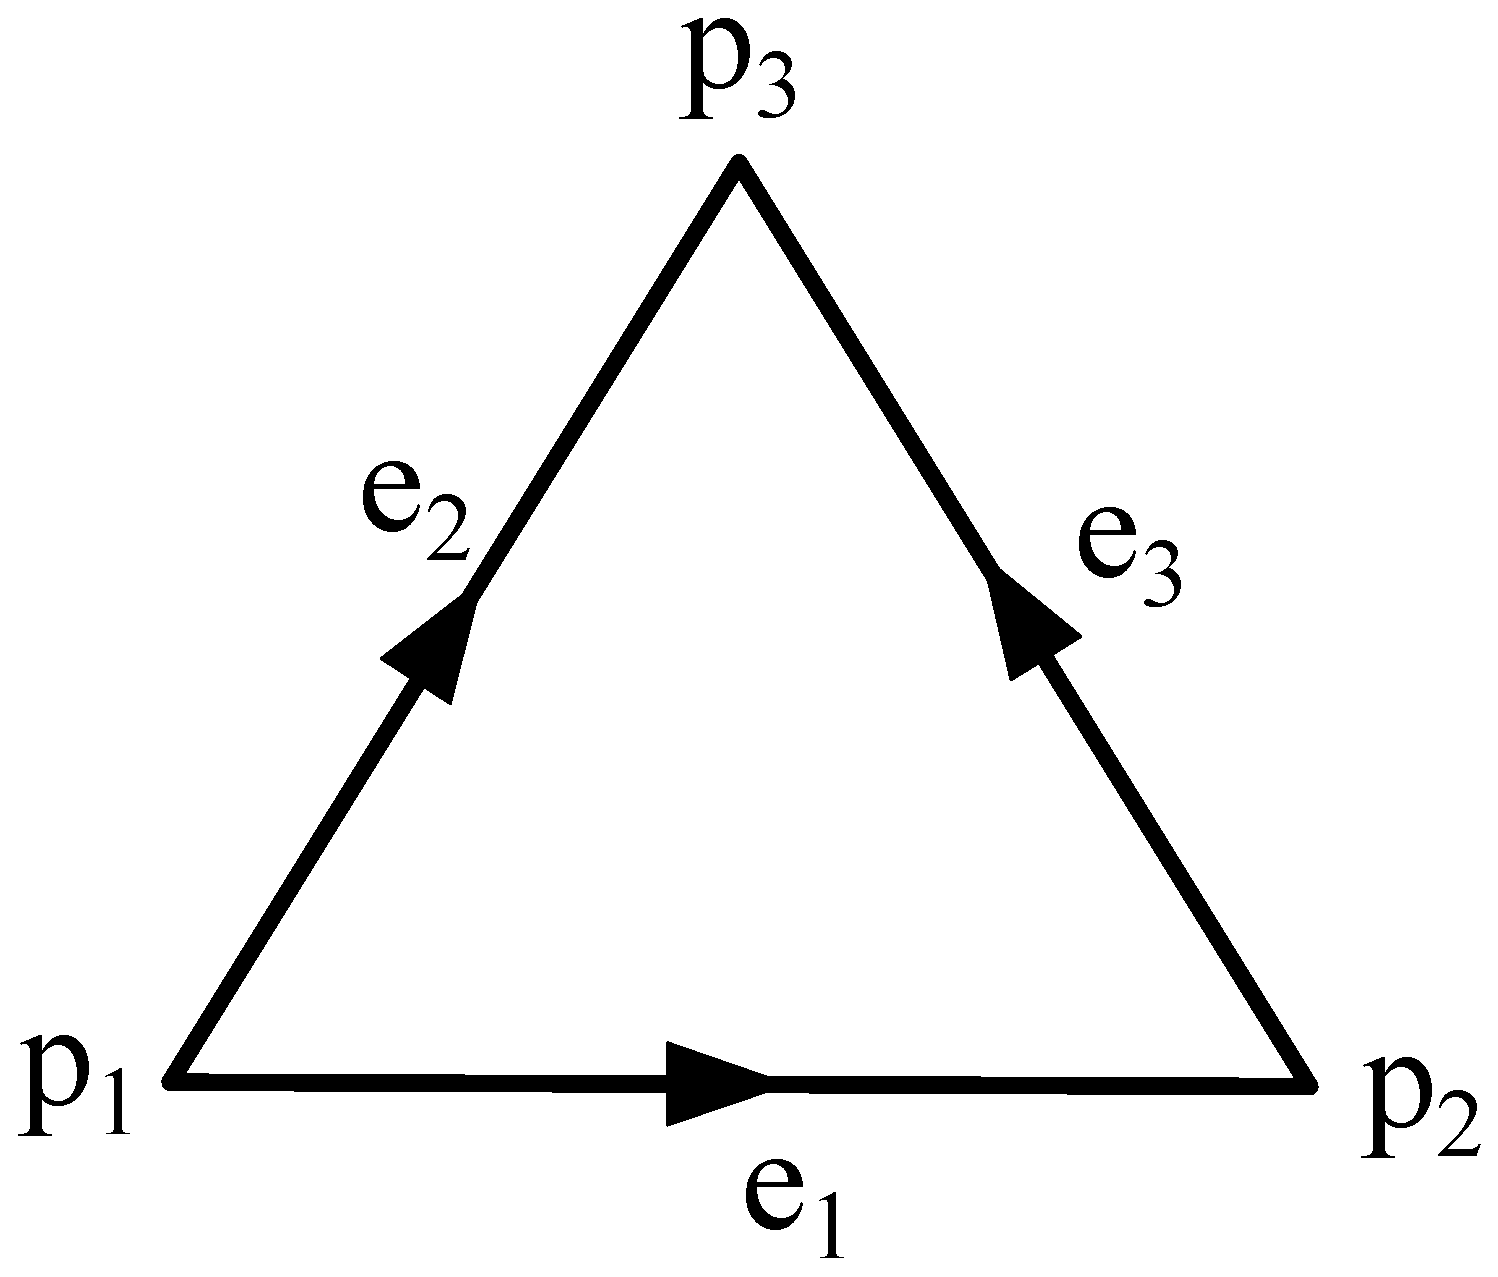
\includegraphics[scale=0.25]{theory/triangle.eps}
	\caption{треугольный конечный элемент}
	\label{fig:theory:triangle}
\end{figure}

\noindent Тогда $\mathcal{L}$-координаты примут вид:
\begin{equation*}
	\mathcal{L}_i (x, y) = \alpha_{i, 1} x + \alpha_{i, 2} y + \alpha_{i, 3} , \text{~~~} i = \overline{1..3} . \label{eq:tr:L}
\end{equation*}
Коэффициенты $\alpha_{i, j}$ могут быть определены по формуле (\ref{eq:tr:D1}):
\begin{equation}
	\left[
	\begin{matrix}
		\alpha_{1, 1} & \alpha_{1, 2} & \alpha_{1, 3} \\
		\alpha_{2, 1} & \alpha_{2, 2} & \alpha_{2, 3} \\
		\alpha_{3, 1} & \alpha_{3, 2} & \alpha_{3, 3} \\
	\end{matrix}
	\right] = \left[
	\begin{matrix}
		{p_1}_x & {p_2}_x & {p_3}_x \\
		{p_1}_y & {p_2}_y & {p_3}_y \\
		1 & 1 & 1 \\
	\end{matrix}
	\right]^{-1} = D^{-1} . \label{eq:tr:D1}
\end{equation}

Иерархический векторный базис Вебба второго порядка второго типа на треугольниках имеет вид:
\begin{equation*}
	\begin{matrix}
		\displaystyle
		\mathbf{w}_{i}^{1,\mathrm{I}} = \mathcal{L}_k \nabla \mathcal{L}_l - \mathcal{L}_l \nabla \mathcal{L}_k ;
		\scriptstyle
		\text{~~} i = 1, ..., 3 ; \text{~~} k, l = 1, ..., 3 ; \text{~~} k < l ,\\
		\displaystyle
		\mathbf{w}_{i}^{1,\mathrm{II}} = \mathcal{L}_k \nabla \mathcal{L}_l + \mathcal{L}_l \nabla \mathcal{L}_k ;
		\scriptstyle
		\text{~~} i = 4, ..., 6 ; \text{~~} k, l = 1, ..., 3 ; \text{~~} k < l ,\\
		\displaystyle
		\mathbf{w}_{7}^{2,\mathrm{I}} = \mathcal{L}_2 \mathcal{L}_3 \nabla \mathcal{L}_1 + \mathcal{L}_1 \mathcal{L}_3 \nabla \mathcal{L}_2 - 2 \mathcal{L}_1 \mathcal{L}_2 \nabla \mathcal{L}_3 ,\\
		\displaystyle
		\mathbf{w}_{8}^{2,\mathrm{I}} = \mathcal{L}_2 \mathcal{L}_3 \nabla \mathcal{L}_1 - 2 \mathcal{L}_1 \mathcal{L}_3 \nabla \mathcal{L}_2 + \mathcal{L}_1 \mathcal{L}_2 \nabla \mathcal{L}_3 ,\\
		\displaystyle
		\mathbf{w}_{9}^{2,\mathrm{II}} = \nabla ( \mathcal{L}_1 \mathcal{L}_2 \mathcal{L}_3 ) ,\\
		\displaystyle
		\mathbf{w}_{i}^{2,\mathrm{II}} = \nabla ( \mathcal{L}_j \mathcal{L}_k ( \mathcal{L}_j - \mathcal{L}_k ) ) ;
		\scriptstyle
		\text{~~} i = 10, ..., 12 ; \text{~~} j, k = 1, ..., 3 ; \text{~~} j < k ,
	\end{matrix}
	\label{eq:tr_basis}
\end{equation*}
где $\mathbf{w}_{1}^{1,\mathrm{I}}, ..., \mathbf{w}_{3}^{1,\mathrm{I}}$ -- базисные функции первого порядка первого типа, $\mathbf{w}_{4}^{1,\mathrm{II}}, ..., \mathbf{w}_{6}^{1,\mathrm{II}}$ -- базисные функции первого порядка второго типа, $\mathbf{w}_{7}^{2,\mathrm{I}}, \mathbf{w}_{8}^{2,\mathrm{I}}$ -- базисные функции второго порядка первого типа, $\mathbf{w}_{9}^{2,\mathrm{II}}, ..., \mathbf{w}_{12}^{2,\mathrm{II}}$ -- базисные функции второго порядка второго типа. Для базиса первого порядка второго типа следует использовать функции $\mathbf{w}_{1}^{1,\mathrm{I}}, ..., \mathbf{w}_{6}^{1,\mathrm{II}}$.

Для вычисления интегралов в (\ref{eq:bound_mnk}) воспользуемся формулой Гаусса~\citep{misovskih}:
\begin{equation*}
	\int\limits_{\Omega_k} f(x, y) \,d\Omega_k = \sum\limits_{i = 1}^m f( x_i , y_i) w_i ,
\end{equation*}
где $(x_i , y_i)$ -- точки Гаусса, $m$ -- число точек Гаусса, $w_i$ -- соответствующие веса. Так же, как и для тетраэдров, для работы с базисом второго порядка нужно использовать формулы, обеспечивающие восьмой порядок интегрирования~\citep{zhang_integration}. Для базиса первого порядка достаточно и меньших порядков интегрирования~\citep{tr_integration, misovskih}.

% =============================================================================

\subsection{Двухуровневый решатель}
%TODO Написать про двухуровневый решатель
{\color{red}\textbf{Написать про двухуровневый решатель}}

% =============================================================================

\clearpage
\section{Построение СЛАУ}
\subsection{Структура глобальной матрицы СЛАУ}
Рассмотрим структуру глобальной матрицы СЛАУ на примере двух тетраэдральных конечных элементов с базисом первого полного порядка, имеющих общую грань. Глобальная нумерация вершин и ребер этих тетраэдров приведена на рисунке \ref{fig:theory:2-tetrahedrons}.
\begin{figure}[H]
	\centering
	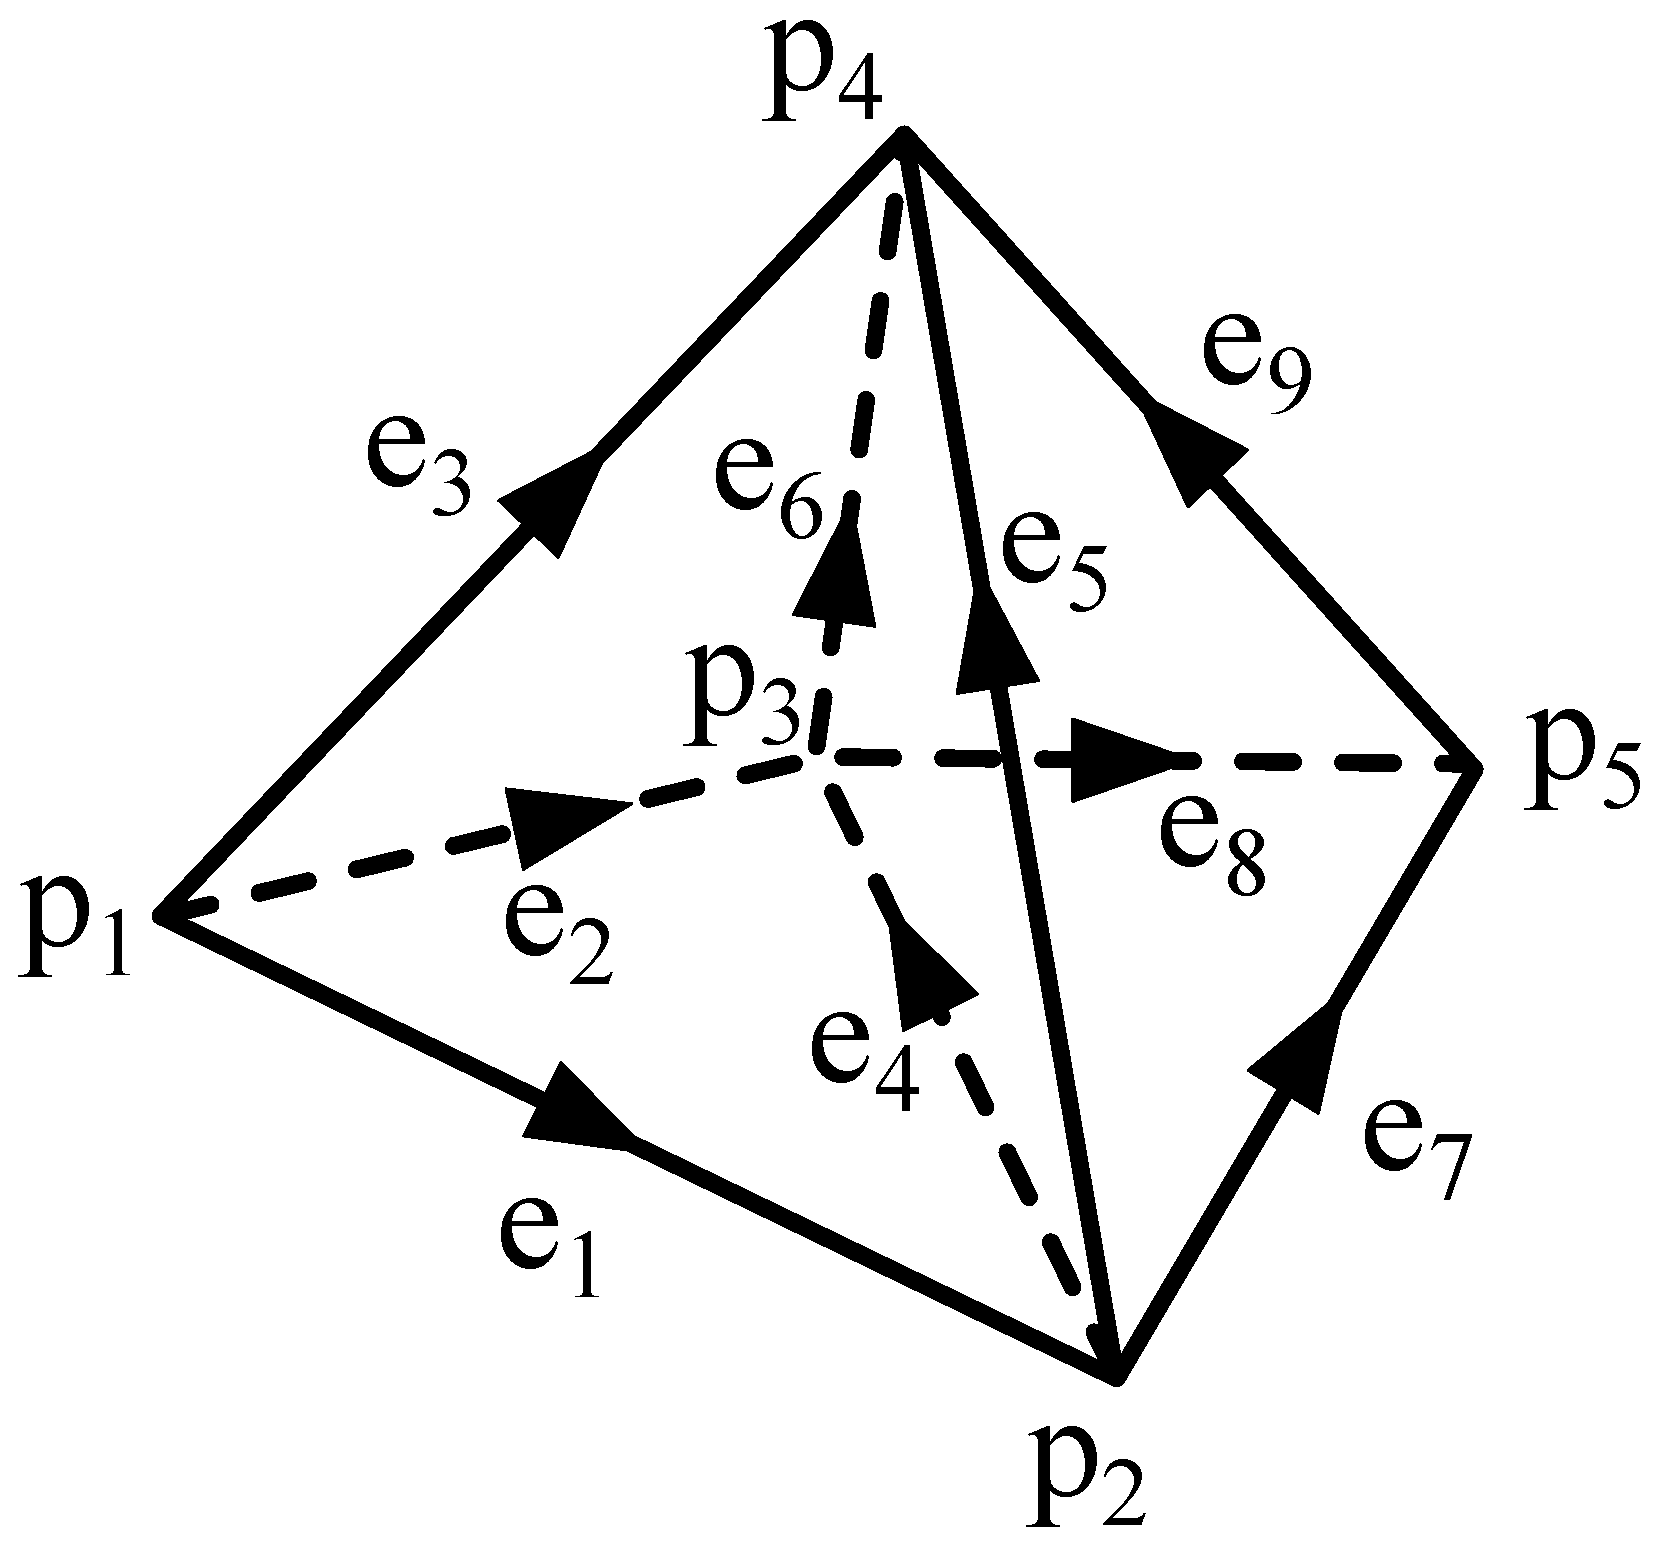
\includegraphics[scale=0.25]{theory/2-tetrahedrons.eps}
	\caption{два тетраэдральных конечных элемента}
	\label{fig:theory:2-tetrahedrons}
\end{figure}

Локальные матрицы тетраэдра имеют блочный вид, матрица массы является плотной (\ref{eq:theory:matrix_M}), а в матрице жесткости ненулевой только один блок (\ref{eq:theory:matrix_G}):
\begin{equation}
	M = \left[
	\begin{matrix}
		M^{I, I} & M^{I, II} \\
		M^{II, I} & M^{II, II} \\
	\end{matrix}
	\right] , \label{eq:theory:matrix_M}
\end{equation}
\begin{equation}
	G = \left[
	\begin{matrix}
		G^{I, I} & \mathbb{O} \\
		 \mathbb{O} &  \mathbb{O} \\
	\end{matrix}
	\right] , \label{eq:theory:matrix_G}
\end{equation}
где $M^{I, I}$, $G^{I, I}$ -- вклады от интегралов, содержащих только роторные ($\mathbf{w}_{1}^{1,\mathrm{I}}, ..., \mathbf{w}_{6}^{1,\mathrm{I}}$); $M^{II, II}$ -- только градиентные ($\mathbf{w}_{7}^{1,\mathrm{II}}, ..., \mathbf{w}_{12}^{1,\mathrm{II}}$); $M^{I, II}$, $M^{II, I}$ -- и роторные, и градиентные базисные функции.

Глобальной матрице жесткости также имеет блочную структуру, для двух тетраэдров она схематично приведена на рисунке \ref{fig:theory:matrx_structure}. Под $G_1$ и $G_2$ понимаются вклады от матриц жесткости (\ref{eq:theory:matrix_G}) первого и второго тетраэдров соответственно, под $M_1$ и $M_2$ -- вклады от матриц массы (\ref{eq:theory:matrix_M}) первого и второго тетраэдров соответственно.

\begin{figure}[H]
	\begin{spacing}{0.75}
	\setlength{\parskip}{0pt}
	\begin{tabu}{|[2pt]@{}C{1}|@{}C{1}|@{}C{1}|@{}C{1}|@{}C{1}|@{}C{1}|@{}C{1}|@{}C{1}|@{}C{1}|[1.25pt]@{}C{1}|@{}C{1}|@{}C{1}|@{}C{1}|@{}C{1}|@{}C{1}|@{}C{1}|@{}C{1}|@{}C{1}|[2pt]}
		\tabucline[2pt]{-}
			~\vspace{-1ex}\par\small $\scriptscriptstyle G_{1} + M_{1}$ &
			~\vspace{-1ex}\par\small $\scriptscriptstyle G_{1} + M_{1}$ &
			~\vspace{-1ex}\par\small $\scriptscriptstyle G_{1} + M_{1}$ &
			~\vspace{-1ex}\par\small $\scriptscriptstyle G_{1} + M_{1}$ &
			~\vspace{-1ex}\par\small $\scriptscriptstyle G_{1} + M_{1}$ &
			~\vspace{-1ex}\par\small $\scriptscriptstyle G_{1} + M_{1}$ &
			&
			&
			&
			~\vspace{-1ex}\par~~\small $\scriptscriptstyle M_{1}$ &
			~\vspace{-1ex}\par~~\small $\scriptscriptstyle M_{1}$ &
			~\vspace{-1ex}\par~~\small $\scriptscriptstyle M_{1}$ &
			~\vspace{-1ex}\par~~\small $\scriptscriptstyle M_{1}$ &
			~\vspace{-1ex}\par~~\small $\scriptscriptstyle M_{1}$ &
			~\vspace{-1ex}\par~~\small $\scriptscriptstyle M_{1}$ &
			&
			&
		\\[0.75ex]\hline
			~\vspace{-1ex}\par\small $\scriptscriptstyle G_{1} + M_{1}$ &
			~\vspace{-1ex}\par\small $\scriptscriptstyle G_{1} + M_{1}$ &
			~\vspace{-1ex}\par\small $\scriptscriptstyle G_{1} + M_{1}$ &
			~\vspace{-1ex}\par\small $\scriptscriptstyle G_{1} + M_{1}$ &
			~\vspace{-1ex}\par\small $\scriptscriptstyle G_{1} + M_{1}$ &
			~\vspace{-1ex}\par\small $\scriptscriptstyle G_{1} + M_{1}$ &
			&
			&
			&
			~\vspace{-1ex}\par~~\small $\scriptscriptstyle M_{1}$ &
			~\vspace{-1ex}\par~~\small $\scriptscriptstyle M_{1}$ &
			~\vspace{-1ex}\par~~\small $\scriptscriptstyle M_{1}$ &
			~\vspace{-1ex}\par~~\small $\scriptscriptstyle M_{1}$ &
			~\vspace{-1ex}\par~~\small $\scriptscriptstyle M_{1}$ &
			~\vspace{-1ex}\par~~\small $\scriptscriptstyle M_{1}$ &
			&
			&
		\\[0.75ex]\hline
			~\vspace{-1ex}\par\small $\scriptscriptstyle G_{1} + M_{1}$ &
			~\vspace{-1ex}\par\small $\scriptscriptstyle G_{1} + M_{1}$ &
			~\vspace{-1ex}\par\small $\scriptscriptstyle G_{1} + M_{1}$ &
			~\vspace{-1ex}\par\small $\scriptscriptstyle G_{1} + M_{1}$ &
			~\vspace{-1ex}\par\small $\scriptscriptstyle G_{1} + M_{1}$ &
			~\vspace{-1ex}\par\small $\scriptscriptstyle G_{1} + M_{1}$ &
			&
			&
			&
			~\vspace{-1ex}\par~~\small $\scriptscriptstyle M_{1}$ &
			~\vspace{-1ex}\par~~\small $\scriptscriptstyle M_{1}$ &
			~\vspace{-1ex}\par~~\small $\scriptscriptstyle M_{1}$ &
			~\vspace{-1ex}\par~~\small $\scriptscriptstyle M_{1}$ &
			~\vspace{-1ex}\par~~\small $\scriptscriptstyle M_{1}$ &
			~\vspace{-1ex}\par~~\small $\scriptscriptstyle M_{1}$ &
			&
			&
		\\[0.75ex]\hline
			~\vspace{-1ex}\par\small $\scriptscriptstyle G_{1} + M_{1}$ &
			~\vspace{-1ex}\par\small $\scriptscriptstyle G_{1} + M_{1}$ &
			~\vspace{-1ex}\par\small $\scriptscriptstyle G_{1} + M_{1}$ &
			~\vspace{-2ex}\par\small $\scriptscriptstyle G_{1} + M_{1}$ \par $\scriptscriptstyle G_{2} + M_{2}$ &
			~\vspace{-2ex}\par\small $\scriptscriptstyle G_{1} + M_{1}$ \par $\scriptscriptstyle G_{2} + M_{2}$ &
			~\vspace{-2ex}\par\small $\scriptscriptstyle G_{1} + M_{1}$ \par $\scriptscriptstyle G_{2} + M_{2}$ &
			~\vspace{-1ex}\par\small $\scriptscriptstyle G_{2} + M_{2}$ &
			~\vspace{-1ex}\par\small $\scriptscriptstyle G_{2} + M_{2}$ &
			~\vspace{-1ex}\par\small $\scriptscriptstyle G_{2} + M_{2}$ &
			~\vspace{-1ex}\par~~\small $\scriptscriptstyle M_{1}$ &
			~\vspace{-1ex}\par~~\small $\scriptscriptstyle M_{1}$ &
			~\vspace{-1ex}\par~~\small $\scriptscriptstyle M_{1}$ &
			~\vspace{-2ex}\par~~\small $\scriptscriptstyle M_{1}$ \par ~~\small $\scriptscriptstyle M_{2}$ &
			~\vspace{-2ex}\par~~\small $\scriptscriptstyle M_{1}$ \par ~~\small $\scriptscriptstyle M_{2}$ &
			~\vspace{-2ex}\par~~\small $\scriptscriptstyle M_{1}$ \par ~~\small $\scriptscriptstyle M_{2}$ &
			~\vspace{-1ex}\par~~\small $\scriptscriptstyle M_{2}$ &
			~\vspace{-1ex}\par~~\small $\scriptscriptstyle M_{2}$ &
			~\vspace{-1ex}\par~~\small $\scriptscriptstyle M_{2}$
		\\[0.25ex]\hline
			~\vspace{-1ex}\par\small $\scriptscriptstyle G_{1} + M_{1}$ &
			~\vspace{-1ex}\par\small $\scriptscriptstyle G_{1} + M_{1}$ &
			~\vspace{-1ex}\par\small $\scriptscriptstyle G_{1} + M_{1}$ &
			~\vspace{-2ex}\par\small $\scriptscriptstyle G_{1} + M_{1}$ \par $\scriptscriptstyle G_{2} + M_{2}$ &
			~\vspace{-2ex}\par\small $\scriptscriptstyle G_{1} + M_{1}$ \par $\scriptscriptstyle G_{2} + M_{2}$ &
			~\vspace{-2ex}\par\small $\scriptscriptstyle G_{1} + M_{1}$ \par $\scriptscriptstyle G_{2} + M_{2}$ &
			~\vspace{-1ex}\par\small $\scriptscriptstyle G_{2} + M_{2}$ &
			~\vspace{-1ex}\par\small $\scriptscriptstyle G_{2} + M_{2}$ &
			~\vspace{-1ex}\par\small $\scriptscriptstyle G_{2} + M_{2}$ &
			~\vspace{-1ex}\par~~\small $\scriptscriptstyle M_{1}$ &
			~\vspace{-1ex}\par~~\small $\scriptscriptstyle M_{1}$ &
			~\vspace{-1ex}\par~~\small $\scriptscriptstyle M_{1}$ &
			~\vspace{-2ex}\par~~\small $\scriptscriptstyle M_{1}$ \par ~~\small $\scriptscriptstyle M_{2}$ &
			~\vspace{-2ex}\par~~\small $\scriptscriptstyle M_{1}$ \par ~~\small $\scriptscriptstyle M_{2}$ &
			~\vspace{-2ex}\par~~\small $\scriptscriptstyle M_{1}$ \par ~~\small $\scriptscriptstyle M_{2}$ &
			~\vspace{-1ex}\par~~\small $\scriptscriptstyle M_{2}$ &
			~\vspace{-1ex}\par~~\small $\scriptscriptstyle M_{2}$ &
			~\vspace{-1ex}\par~~\small $\scriptscriptstyle M_{2}$
		\\[0.25ex]\hline
			~\vspace{-1ex}\par\small $\scriptscriptstyle G_{1} + M_{1}$ &
			~\vspace{-1ex}\par\small $\scriptscriptstyle G_{1} + M_{1}$ &
			~\vspace{-1ex}\par\small $\scriptscriptstyle G_{1} + M_{1}$ &
			~\vspace{-2ex}\par\small $\scriptscriptstyle G_{1} + M_{1}$ \par $\scriptscriptstyle G_{2} + M_{2}$ &
			~\vspace{-2ex}\par\small $\scriptscriptstyle G_{1} + M_{1}$ \par $\scriptscriptstyle G_{2} + M_{2}$ &
			~\vspace{-2ex}\par\small $\scriptscriptstyle G_{1} + M_{1}$ \par $\scriptscriptstyle G_{2} + M_{2}$ &
			~\vspace{-1ex}\par\small $\scriptscriptstyle G_{2} + M_{2}$ &
			~\vspace{-1ex}\par\small $\scriptscriptstyle G_{2} + M_{2}$ &
			~\vspace{-1ex}\par\small $\scriptscriptstyle G_{2} + M_{2}$ &
			~\vspace{-1ex}\par~~\small $\scriptscriptstyle M_{1}$ &
			~\vspace{-1ex}\par~~\small $\scriptscriptstyle M_{1}$ &
			~\vspace{-1ex}\par~~\small $\scriptscriptstyle M_{1}$ &
			~\vspace{-2ex}\par~~\small $\scriptscriptstyle M_{1}$ \par ~~\small $\scriptscriptstyle M_{2}$ &
			~\vspace{-2ex}\par~~\small $\scriptscriptstyle M_{1}$ \par ~~\small $\scriptscriptstyle M_{2}$ &
			~\vspace{-2ex}\par~~\small $\scriptscriptstyle M_{1}$ \par ~~\small $\scriptscriptstyle M_{2}$ &
			~\vspace{-1ex}\par~~\small $\scriptscriptstyle M_{2}$ &
			~\vspace{-1ex}\par~~\small $\scriptscriptstyle M_{2}$ &
			~\vspace{-1ex}\par~~\small $\scriptscriptstyle M_{2}$
		\\[0.25ex]\hline
			&
			&
			&
			~\vspace{-1ex}\par\small $\scriptscriptstyle G_{2} + M_{2}$ &
			~\vspace{-1ex}\par\small $\scriptscriptstyle G_{2} + M_{2}$ &
			~\vspace{-1ex}\par\small $\scriptscriptstyle G_{2} + M_{2}$ &
			~\vspace{-1ex}\par\small $\scriptscriptstyle G_{2} + M_{2}$ &
			~\vspace{-1ex}\par\small $\scriptscriptstyle G_{2} + M_{2}$ &
			~\vspace{-1ex}\par\small $\scriptscriptstyle G_{2} + M_{2}$ &
			&
			&
			&
			~\vspace{-1ex}\par~~\small $\scriptscriptstyle M_{2}$ &
			~\vspace{-1ex}\par~~\small $\scriptscriptstyle M_{2}$ &
			~\vspace{-1ex}\par~~\small $\scriptscriptstyle M_{2}$ &
			~\vspace{-1ex}\par~~\small $\scriptscriptstyle M_{2}$ &
			~\vspace{-1ex}\par~~\small $\scriptscriptstyle M_{2}$ &
			~\vspace{-1ex}\par~~\small $\scriptscriptstyle M_{2}$
		\\[0.25ex]\hline
			&
			&
			&
			~\vspace{-1ex}\par\small $\scriptscriptstyle G_{2} + M_{2}$ &
			~\vspace{-1ex}\par\small $\scriptscriptstyle G_{2} + M_{2}$ &
			~\vspace{-1ex}\par\small $\scriptscriptstyle G_{2} + M_{2}$ &
			~\vspace{-1ex}\par\small $\scriptscriptstyle G_{2} + M_{2}$ &
			~\vspace{-1ex}\par\small $\scriptscriptstyle G_{2} + M_{2}$ &
			~\vspace{-1ex}\par\small $\scriptscriptstyle G_{2} + M_{2}$ &
			&
			&
			&
			~\vspace{-1ex}\par~~\small $\scriptscriptstyle M_{2}$ &
			~\vspace{-1ex}\par~~\small $\scriptscriptstyle M_{2}$ &
			~\vspace{-1ex}\par~~\small $\scriptscriptstyle M_{2}$ &
			~\vspace{-1ex}\par~~\small $\scriptscriptstyle M_{2}$ &
			~\vspace{-1ex}\par~~\small $\scriptscriptstyle M_{2}$ &
			~\vspace{-1ex}\par~~\small $\scriptscriptstyle M_{2}$
		\\[0.25ex]\hline
			&
			&
			&
			~\vspace{-1ex}\par\small $\scriptscriptstyle G_{2} + M_{2}$ &
			~\vspace{-1ex}\par\small $\scriptscriptstyle G_{2} + M_{2}$ &
			~\vspace{-1ex}\par\small $\scriptscriptstyle G_{2} + M_{2}$ &
			~\vspace{-1ex}\par\small $\scriptscriptstyle G_{2} + M_{2}$ &
			~\vspace{-1ex}\par\small $\scriptscriptstyle G_{2} + M_{2}$ &
			~\vspace{-1ex}\par\small $\scriptscriptstyle G_{2} + M_{2}$ &
			&
			&
			&
			~\vspace{-1ex}\par~~\small $\scriptscriptstyle M_{2}$ &
			~\vspace{-1ex}\par~~\small $\scriptscriptstyle M_{2}$ &
			~\vspace{-1ex}\par~~\small $\scriptscriptstyle M_{2}$ &
			~\vspace{-1ex}\par~~\small $\scriptscriptstyle M_{2}$ &
			~\vspace{-1ex}\par~~\small $\scriptscriptstyle M_{2}$ &
			~\vspace{-1ex}\par~~\small $\scriptscriptstyle M_{2}$
		\\[0.25ex]\tabucline[1.25pt]{-}
			~\vspace{-1ex}\par~~\small $\scriptscriptstyle M_{1}$ &
			~\vspace{-1ex}\par~~\small $\scriptscriptstyle M_{1}$ &
			~\vspace{-1ex}\par~~\small $\scriptscriptstyle M_{1}$ &
			~\vspace{-1ex}\par~~\small $\scriptscriptstyle M_{1}$ &
			~\vspace{-1ex}\par~~\small $\scriptscriptstyle M_{1}$ &
			~\vspace{-1ex}\par~~\small $\scriptscriptstyle M_{1}$ &
			&
			&
			&
			~\vspace{-1ex}\par~~\small $\scriptscriptstyle M_{1}$ &
			~\vspace{-1ex}\par~~\small $\scriptscriptstyle M_{1}$ &
			~\vspace{-1ex}\par~~\small $\scriptscriptstyle M_{1}$ &
			~\vspace{-1ex}\par~~\small $\scriptscriptstyle M_{1}$ &
			~\vspace{-1ex}\par~~\small $\scriptscriptstyle M_{1}$ &
			~\vspace{-1ex}\par~~\small $\scriptscriptstyle M_{1}$ &
			&
			&
		\\[0.75ex]\hline
			~\vspace{-1ex}\par~~\small $\scriptscriptstyle M_{1}$ &
			~\vspace{-1ex}\par~~\small $\scriptscriptstyle M_{1}$ &
			~\vspace{-1ex}\par~~\small $\scriptscriptstyle M_{1}$ &
			~\vspace{-1ex}\par~~\small $\scriptscriptstyle M_{1}$ &
			~\vspace{-1ex}\par~~\small $\scriptscriptstyle M_{1}$ &
			~\vspace{-1ex}\par~~\small $\scriptscriptstyle M_{1}$ &
			&
			&
			&
			~\vspace{-1ex}\par~~\small $\scriptscriptstyle M_{1}$ &
			~\vspace{-1ex}\par~~\small $\scriptscriptstyle M_{1}$ &
			~\vspace{-1ex}\par~~\small $\scriptscriptstyle M_{1}$ &
			~\vspace{-1ex}\par~~\small $\scriptscriptstyle M_{1}$ &
			~\vspace{-1ex}\par~~\small $\scriptscriptstyle M_{1}$ &
			~\vspace{-1ex}\par~~\small $\scriptscriptstyle M_{1}$ &
			&
			&
		\\[0.75ex]\hline
			~\vspace{-1ex}\par~~\small $\scriptscriptstyle M_{1}$ &
			~\vspace{-1ex}\par~~\small $\scriptscriptstyle M_{1}$ &
			~\vspace{-1ex}\par~~\small $\scriptscriptstyle M_{1}$ &
			~\vspace{-1ex}\par~~\small $\scriptscriptstyle M_{1}$ &
			~\vspace{-1ex}\par~~\small $\scriptscriptstyle M_{1}$ &
			~\vspace{-1ex}\par~~\small $\scriptscriptstyle M_{1}$ &
			&
			&
			&
			~\vspace{-1ex}\par~~\small $\scriptscriptstyle M_{1}$ &
			~\vspace{-1ex}\par~~\small $\scriptscriptstyle M_{1}$ &
			~\vspace{-1ex}\par~~\small $\scriptscriptstyle M_{1}$ &
			~\vspace{-1ex}\par~~\small $\scriptscriptstyle M_{1}$ &
			~\vspace{-1ex}\par~~\small $\scriptscriptstyle M_{1}$ &
			~\vspace{-1ex}\par~~\small $\scriptscriptstyle M_{1}$ &
			&
			&
		\\[0.75ex]\hline
			~\vspace{-1ex}\par~~\small $\scriptscriptstyle M_{1}$ &
			~\vspace{-1ex}\par~~\small $\scriptscriptstyle M_{1}$ &
			~\vspace{-1ex}\par~~\small $\scriptscriptstyle M_{1}$ &
			~\vspace{-2ex}\par~~\small $\scriptscriptstyle M_{1}$ \par ~~\small $\scriptscriptstyle M_{2}$ &
			~\vspace{-2ex}\par~~\small $\scriptscriptstyle M_{1}$ \par ~~\small $\scriptscriptstyle M_{2}$ &
			~\vspace{-2ex}\par~~\small $\scriptscriptstyle M_{1}$ \par ~~\small $\scriptscriptstyle M_{2}$ &
			~\vspace{-1ex}\par~~\small $\scriptscriptstyle M_{2}$ &
			~\vspace{-1ex}\par~~\small $\scriptscriptstyle M_{2}$ &
			~\vspace{-1ex}\par~~\small $\scriptscriptstyle M_{2}$ &
			~\vspace{-1ex}\par~~\small $\scriptscriptstyle M_{1}$ &
			~\vspace{-1ex}\par~~\small $\scriptscriptstyle M_{1}$ &
			~\vspace{-1ex}\par~~\small $\scriptscriptstyle M_{1}$ &
			~\vspace{-2ex}\par~~\small $\scriptscriptstyle M_{1}$ \par ~~\small $\scriptscriptstyle M_{2}$ &
			~\vspace{-2ex}\par~~\small $\scriptscriptstyle M_{1}$ \par ~~\small $\scriptscriptstyle M_{2}$ &
			~\vspace{-2ex}\par~~\small $\scriptscriptstyle M_{1}$ \par ~~\small $\scriptscriptstyle M_{2}$ &
			~\vspace{-1ex}\par~~\small $\scriptscriptstyle M_{2}$ &
			~\vspace{-1ex}\par~~\small $\scriptscriptstyle M_{2}$ &
			~\vspace{-1ex}\par~~\small $\scriptscriptstyle M_{2}$
		\\[0.25ex]\hline
			~\vspace{-1ex}\par~~\small $\scriptscriptstyle M_{1}$ &
			~\vspace{-1ex}\par~~\small $\scriptscriptstyle M_{1}$ &
			~\vspace{-1ex}\par~~\small $\scriptscriptstyle M_{1}$ &
			~\vspace{-2ex}\par~~\small $\scriptscriptstyle M_{1}$ \par ~~\small $\scriptscriptstyle M_{2}$ &
			~\vspace{-2ex}\par~~\small $\scriptscriptstyle M_{1}$ \par ~~\small $\scriptscriptstyle M_{2}$ &
			~\vspace{-2ex}\par~~\small $\scriptscriptstyle M_{1}$ \par ~~\small $\scriptscriptstyle M_{2}$ &
			~\vspace{-1ex}\par~~\small $\scriptscriptstyle M_{2}$ &
			~\vspace{-1ex}\par~~\small $\scriptscriptstyle M_{2}$ &
			~\vspace{-1ex}\par~~\small $\scriptscriptstyle M_{2}$ &
			~\vspace{-1ex}\par~~\small $\scriptscriptstyle M_{1}$ &
			~\vspace{-1ex}\par~~\small $\scriptscriptstyle M_{1}$ &
			~\vspace{-1ex}\par~~\small $\scriptscriptstyle M_{1}$ &
			~\vspace{-2ex}\par~~\small $\scriptscriptstyle M_{1}$ \par ~~\small $\scriptscriptstyle M_{2}$ &
			~\vspace{-2ex}\par~~\small $\scriptscriptstyle M_{1}$ \par ~~\small $\scriptscriptstyle M_{2}$ &
			~\vspace{-2ex}\par~~\small $\scriptscriptstyle M_{1}$ \par ~~\small $\scriptscriptstyle M_{2}$ &
			~\vspace{-1ex}\par~~\small $\scriptscriptstyle M_{2}$ &
			~\vspace{-1ex}\par~~\small $\scriptscriptstyle M_{2}$ &
			~\vspace{-1ex}\par~~\small $\scriptscriptstyle M_{2}$
		\\[0.25ex]\hline
			~\vspace{-1ex}\par~~\small $\scriptscriptstyle M_{1}$ &
			~\vspace{-1ex}\par~~\small $\scriptscriptstyle M_{1}$ &
			~\vspace{-1ex}\par~~\small $\scriptscriptstyle M_{1}$ &
			~\vspace{-2ex}\par~~\small $\scriptscriptstyle M_{1}$ \par ~~\small $\scriptscriptstyle M_{2}$ &
			~\vspace{-2ex}\par~~\small $\scriptscriptstyle M_{1}$ \par ~~\small $\scriptscriptstyle M_{2}$ &
			~\vspace{-2ex}\par~~\small $\scriptscriptstyle M_{1}$ \par ~~\small $\scriptscriptstyle M_{2}$ &
			~\vspace{-1ex}\par~~\small $\scriptscriptstyle M_{2}$ &
			~\vspace{-1ex}\par~~\small $\scriptscriptstyle M_{2}$ &
			~\vspace{-1ex}\par~~\small $\scriptscriptstyle M_{2}$ &
			~\vspace{-1ex}\par~~\small $\scriptscriptstyle M_{1}$ &
			~\vspace{-1ex}\par~~\small $\scriptscriptstyle M_{1}$ &
			~\vspace{-1ex}\par~~\small $\scriptscriptstyle M_{1}$ &
			~\vspace{-2ex}\par~~\small $\scriptscriptstyle M_{1}$ \par ~~\small $\scriptscriptstyle M_{2}$ &
			~\vspace{-2ex}\par~~\small $\scriptscriptstyle M_{1}$ \par ~~\small $\scriptscriptstyle M_{2}$ &
			~\vspace{-2ex}\par~~\small $\scriptscriptstyle M_{1}$ \par ~~\small $\scriptscriptstyle M_{2}$ &
			~\vspace{-1ex}\par~~\small $\scriptscriptstyle M_{2}$ &
			~\vspace{-1ex}\par~~\small $\scriptscriptstyle M_{2}$ &
			~\vspace{-1ex}\par~~\small $\scriptscriptstyle M_{2}$
		\\[0.25ex]\hline
			&
			&
			&
			~\vspace{-1ex}\par~~\small $\scriptscriptstyle M_{2}$ &
			~\vspace{-1ex}\par~~\small $\scriptscriptstyle M_{2}$ &
			~\vspace{-1ex}\par~~\small $\scriptscriptstyle M_{2}$ &
			~\vspace{-1ex}\par~~\small $\scriptscriptstyle M_{2}$ &
			~\vspace{-1ex}\par~~\small $\scriptscriptstyle M_{2}$ &
			~\vspace{-1ex}\par~~\small $\scriptscriptstyle M_{2}$ &
			&
			&
			&
			~\vspace{-1ex}\par~~\small $\scriptscriptstyle M_{2}$ &
			~\vspace{-1ex}\par~~\small $\scriptscriptstyle M_{2}$ &
			~\vspace{-1ex}\par~~\small $\scriptscriptstyle M_{2}$ &
			~\vspace{-1ex}\par~~\small $\scriptscriptstyle M_{2}$ &
			~\vspace{-1ex}\par~~\small $\scriptscriptstyle M_{2}$ &
			~\vspace{-1ex}\par~~\small $\scriptscriptstyle M_{2}$
		\\[0.25ex]\hline
			&
			&
			&
			~\vspace{-1ex}\par~~\small $\scriptscriptstyle M_{2}$ &
			~\vspace{-1ex}\par~~\small $\scriptscriptstyle M_{2}$ &
			~\vspace{-1ex}\par~~\small $\scriptscriptstyle M_{2}$ &
			~\vspace{-1ex}\par~~\small $\scriptscriptstyle M_{2}$ &
			~\vspace{-1ex}\par~~\small $\scriptscriptstyle M_{2}$ &
			~\vspace{-1ex}\par~~\small $\scriptscriptstyle M_{2}$ &
			&
			&
			&
			~\vspace{-1ex}\par~~\small $\scriptscriptstyle M_{2}$ &
			~\vspace{-1ex}\par~~\small $\scriptscriptstyle M_{2}$ &
			~\vspace{-1ex}\par~~\small $\scriptscriptstyle M_{2}$ &
			~\vspace{-1ex}\par~~\small $\scriptscriptstyle M_{2}$ &
			~\vspace{-1ex}\par~~\small $\scriptscriptstyle M_{2}$ &
			~\vspace{-1ex}\par~~\small $\scriptscriptstyle M_{2}$
		\\[0.25ex]\hline
			&
			&
			&
			~\vspace{-1ex}\par~~\small $\scriptscriptstyle M_{2}$ &
			~\vspace{-1ex}\par~~\small $\scriptscriptstyle M_{2}$ &
			~\vspace{-1ex}\par~~\small $\scriptscriptstyle M_{2}$ &
			~\vspace{-1ex}\par~~\small $\scriptscriptstyle M_{2}$ &
			~\vspace{-1ex}\par~~\small $\scriptscriptstyle M_{2}$ &
			~\vspace{-1ex}\par~~\small $\scriptscriptstyle M_{2}$ &
			&
			&
			&
			~\vspace{-1ex}\par~~\small $\scriptscriptstyle M_{2}$ &
			~\vspace{-1ex}\par~~\small $\scriptscriptstyle M_{2}$ &
			~\vspace{-1ex}\par~~\small $\scriptscriptstyle M_{2}$ &
			~\vspace{-1ex}\par~~\small $\scriptscriptstyle M_{2}$ &
			~\vspace{-1ex}\par~~\small $\scriptscriptstyle M_{2}$ &
			~\vspace{-1ex}\par~~\small $\scriptscriptstyle M_{2}$
		\\[0.25ex]\tabucline[2pt]{-}
	\end{tabu}
	\end{spacing}
	\vspace{1ex}
	\caption{структура СЛАУ}
	\label{fig:theory:matrx_structure}
\end{figure}

% =============================================================================

\subsection{Учет краевых условий}

Неоднородные краевые условия первого рода вида (\ref{eq:bound1}) учитываются следующим образом:
\begin{enumerate}
	\item строится разложение $\mathbf{E}^g$ по базису треугольников границы в смысле МНК, для этого решается СЛАУ вида (\ref{eq:bound_mnk});
	\item в диагональные элементы глобальной матрицы, соответствующие базисным функциям треугольников границы, записываются единицы, в элементы правой части -- полученные веса;
	\item выполняется симметризация СЛАУ (если СЛАУ хранится в несимметричном формате, этот шаг можно пропустить).
\end{enumerate}

Однородные краевые условия первого рода вида (\ref{eq:bound1_zero}) учитываются аналогично, с той лишь разницей, что не требуется строить разложение $\mathbf{E}^g$ по базису, так как очевидно, что все веса будут нулевыми.

Однородные электрические краевые условия второго рода вида (\ref{eq:bound2}) учитываются естественным образом и не вносят вклад в матрицу или правую часть СЛАУ, поэтому не требуют какой-либо специальной процедуры учета.

% =============================================================================

\subsection{Учет токовой петли}
%TODO Написать про учет токовой петли, спросить у Макса если что
{\color{red}\textbf{Написать про учет токовой петли}}

% =============================================================================

\clearpage
\section{Верификация программного комплекса}
Верификация полученной конечноэлементной аппроксимации будет проводиться на тестовой задаче, имеющей аналитическое решение.
\subsection{Расчетная область}
Расчетная область представляет собой куб со следующими параметрами: $x \in [0,1]$, $y \in [0,1]$, $z \in [0,1]$. Куб разбивается на регулярную тетраэдральную сетку согласно рисунку \ref{fig:verify:x1}:

\begin{figure}[!htbp]
%\begin{figure}[H]
	\centering
	% trim=left bottom right top
	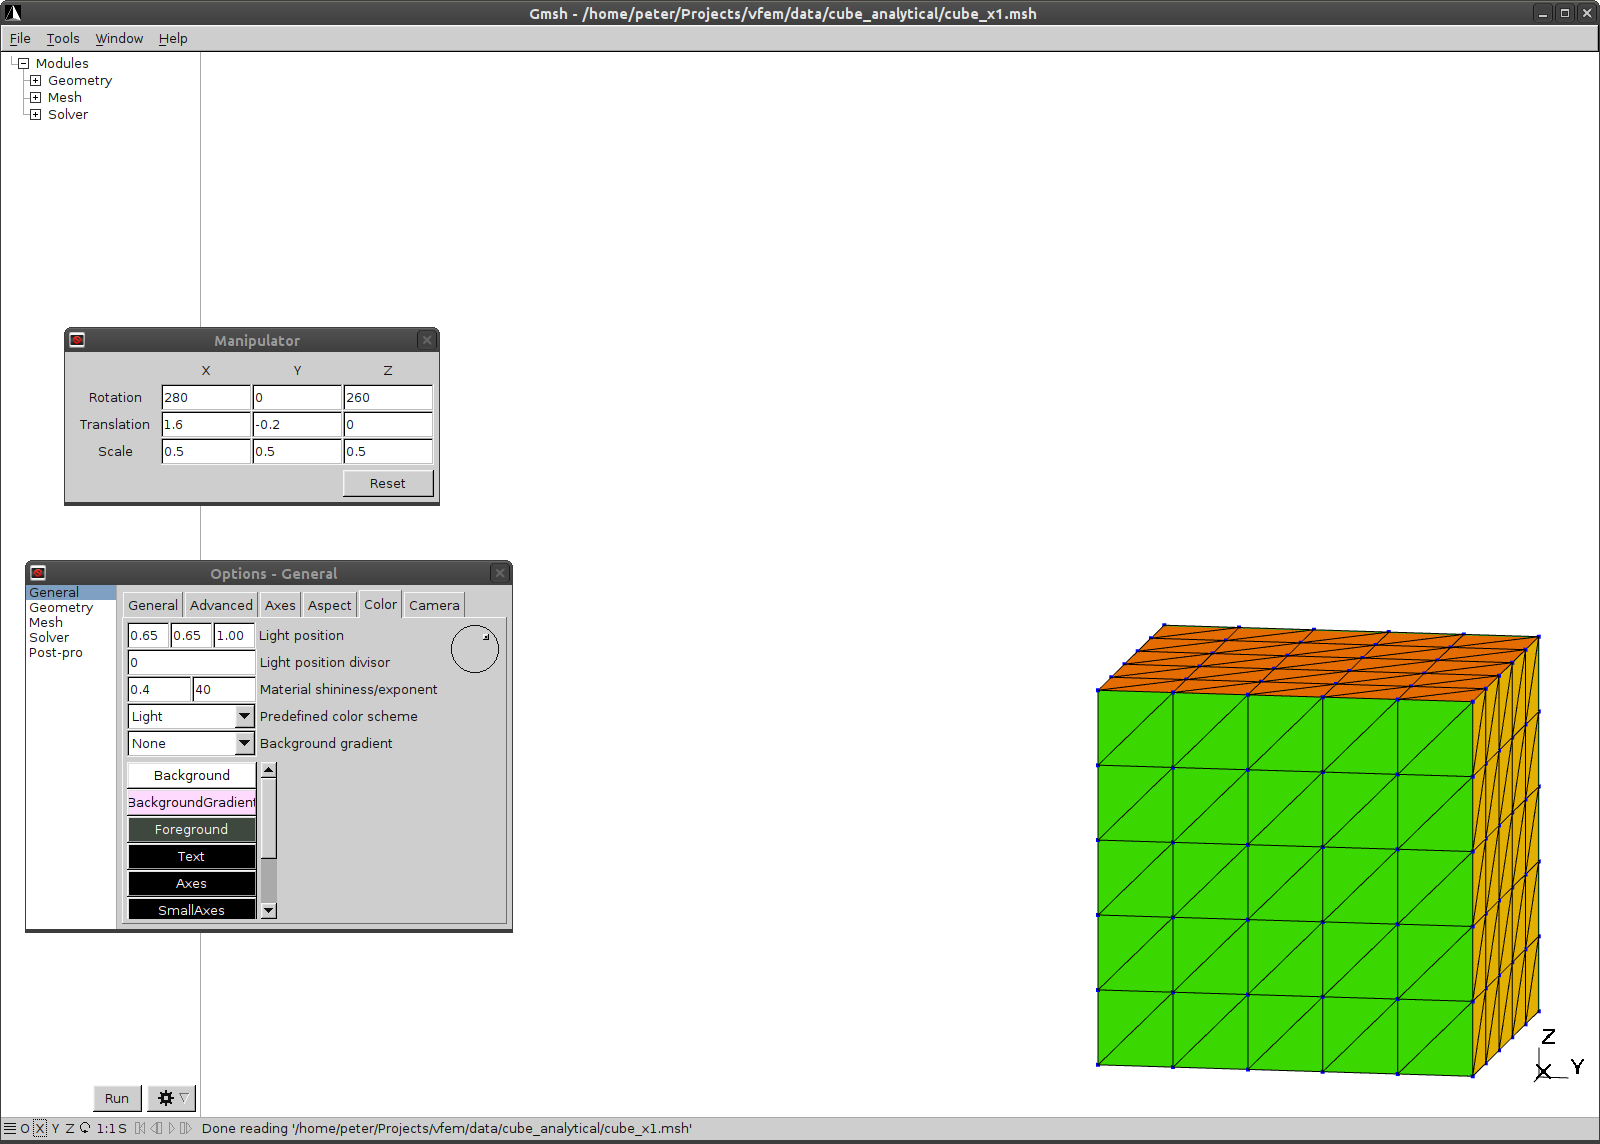
\includegraphics[trim=387mm 20mm 5mm 220mm,clip,scale=0.4]{verify/x1.png}
	\caption{конечноэлементная сетка для верификации}
	\label{fig:verify:x1}
\end{figure}

\noindent Всего в сетке 750 тетраэдров, 300 треугольников по границе, 216 узлов, 1115 ребер и 1650 граней.

Физические параметры среды заданы следующим образом: $\varepsilon = \varepsilon_0$, $\mu = \mu_0$, $\sigma = 10$~См/м. Частота источника поля $\nu = \frac{100}{2 \pi}$~Гц. На всех внешних гранях расчетной области заданы краевые условия первого рода (\ref{eq:bound1}).

% =============================================================================

\subsection{Тестирование на линейных функциях}
В качестве аналитического решения уравнения (\ref{eq:helmholtz}) выберем функцию
\begin{equation*}
	\mathbf{E} = ( y+z , x+z, x+y )^T .
\end{equation*}
Тестирование будем проводить на базисных функциях первого и второго порядка второго типа. Погрешности в норме пространства $\mathbb{L}^2$ полученных решений приведены в таблице \ref{tab:verify:linear_diff}.

\begin{table}[H]
	\caption{относительные погрешности в норме $\mathbb{L}^2$}
	\label{tab:verify:linear_diff}
	\begin{tabularx}{\textwidth}{|C{1}|C{1}|C{1}|C{1}|C{1}|C{1}|}
		\hline Порядок базисных ф-й & \raisebox{-0.7em}{$\smash{\displaystyle \frac{\| |\mathbf{E}| - |\mathbf{E}^h| \|_{\mathbb{L}^2}}{\| |\mathbf{E}| \|_{\mathbb{L}^2}}}$} & \raisebox{-0.7em}{$\smash{\displaystyle \frac{\| \mathbf{E}_x - \mathbf{E}^h_x \|_{\mathbb{L}^2}}{\| \mathbf{E}_x \|_{\mathbb{L}^2}}}$} & \raisebox{-0.7em}{$\smash{\displaystyle \frac{\| \mathbf{E}_y - \mathbf{E}^h_y \|_{\mathbb{L}^2}}{\| \mathbf{E}_y \|_{\mathbb{L}^2}}}$} & \raisebox{-0.7em}{$\smash{\displaystyle \frac{\| \mathbf{E}_z - \mathbf{E}^h_z \|_{\mathbb{L}^2}}{\| \mathbf{E}_z \|_{\mathbb{L}^2}}}$} \\
		\hline 1 & 5.277e-11 & 5.313e-11 & 5.345e-11 & 5.169e-11 \\
		\hline 2 & 8.064e-11 & 8.111e-11 & 8.056e-11 & 8.025e-11 \\
		\hline
	\end{tabularx}
\end{table}
\vspace{-0.5cm}Как и следовало ожидать, метод хорошо аппроксимировал линейную функцию.

% =============================================================================

\subsection{Тестирование на нелинейных функциях}

В качестве аналитического решения уравнения (\ref{eq:helmholtz}) выберем функцию
\begin{equation}
	\mathbf{E} = \left( \begin{array}{c}
		e^{-(0.5-y)^2 -(0.5-z)^2} \\
		e^{-(0.5-x)^2 -(0.5-z)^2} \\
		e^{-(0.5-x)^2 -(0.5-y)^2} \\
	\end{array} \right) .
	\label{eq:verify:exp_solution}
\end{equation}
Тестирование будем проводить на базисных функциях первого и второго порядка второго типа. Погрешности в норме пространства $\mathbb{L}^2$ полученных решений приведены в таблице \ref{tab:verify:exp_diff}.

\begin{table}[H]
	\caption{относительные погрешности в норме $\mathbb{L}^2$}
	\label{tab:verify:exp_diff}
	\begin{tabularx}{\textwidth}{|C{1}|C{1}|C{1}|C{1}|C{1}|C{1}|}
		\hline Порядок базисных ф-й & \raisebox{-0.7em}{$\smash{\displaystyle \frac{\| |\mathbf{E}| - |\mathbf{E}^h| \|_{\mathbb{L}^2}}{\| |\mathbf{E}| \|_{\mathbb{L}^2}}}$} & \raisebox{-0.7em}{$\smash{\displaystyle \frac{\| \mathbf{E}_x - \mathbf{E}^h_x \|_{\mathbb{L}^2}}{\| \mathbf{E}_x \|_{\mathbb{L}^2}}}$} & \raisebox{-0.7em}{$\smash{\displaystyle \frac{\| \mathbf{E}_y - \mathbf{E}^h_y \|_{\mathbb{L}^2}}{\| \mathbf{E}_y \|_{\mathbb{L}^2}}}$} & \raisebox{-0.7em}{$\smash{\displaystyle \frac{\| \mathbf{E}_z - \mathbf{E}^h_z \|_{\mathbb{L}^2}}{\| \mathbf{E}_z \|_{\mathbb{L}^2}}}$} \\
		\hline 1 & 6.608e-3 & 7.869e-3 & 5.877e-3 & 5.877e-3 \\
		\hline 2 & 1.775e-4 & 1.895e-4 & 1.712e-4 & 1.712e-4 \\
		\hline
	\end{tabularx}
\end{table}
\vspace{-0.5cm}Метод достаточно хорошо аппроксимировал и нелинейную функцию.

% =============================================================================

\subsection{Определение порядка аппроксимации}

В качестве аналитического решения уравнения (\ref{eq:helmholtz}) выберем функцию (\ref{eq:verify:exp_solution}). Проведем исследование на порядок аппроксимации. Измельчим сетку расчетной области, изображенную на рисунке \ref{fig:verify:x1}, в 2 и 4 раза, после чего сравним погрешности полученных решений. Измельченные сетки приведены на рисунках \ref{fig:verify:x2} и \ref{fig:verify:x4}, погрешности в норме пространства $\mathbb{L}^2$ полученных решений и порядок аппроксимации -- в таблице \ref{tab:verify:exp_order}.

\begin{figure}[H]
	\centering
	% trim=left bottom right top
	\subfloat[][]{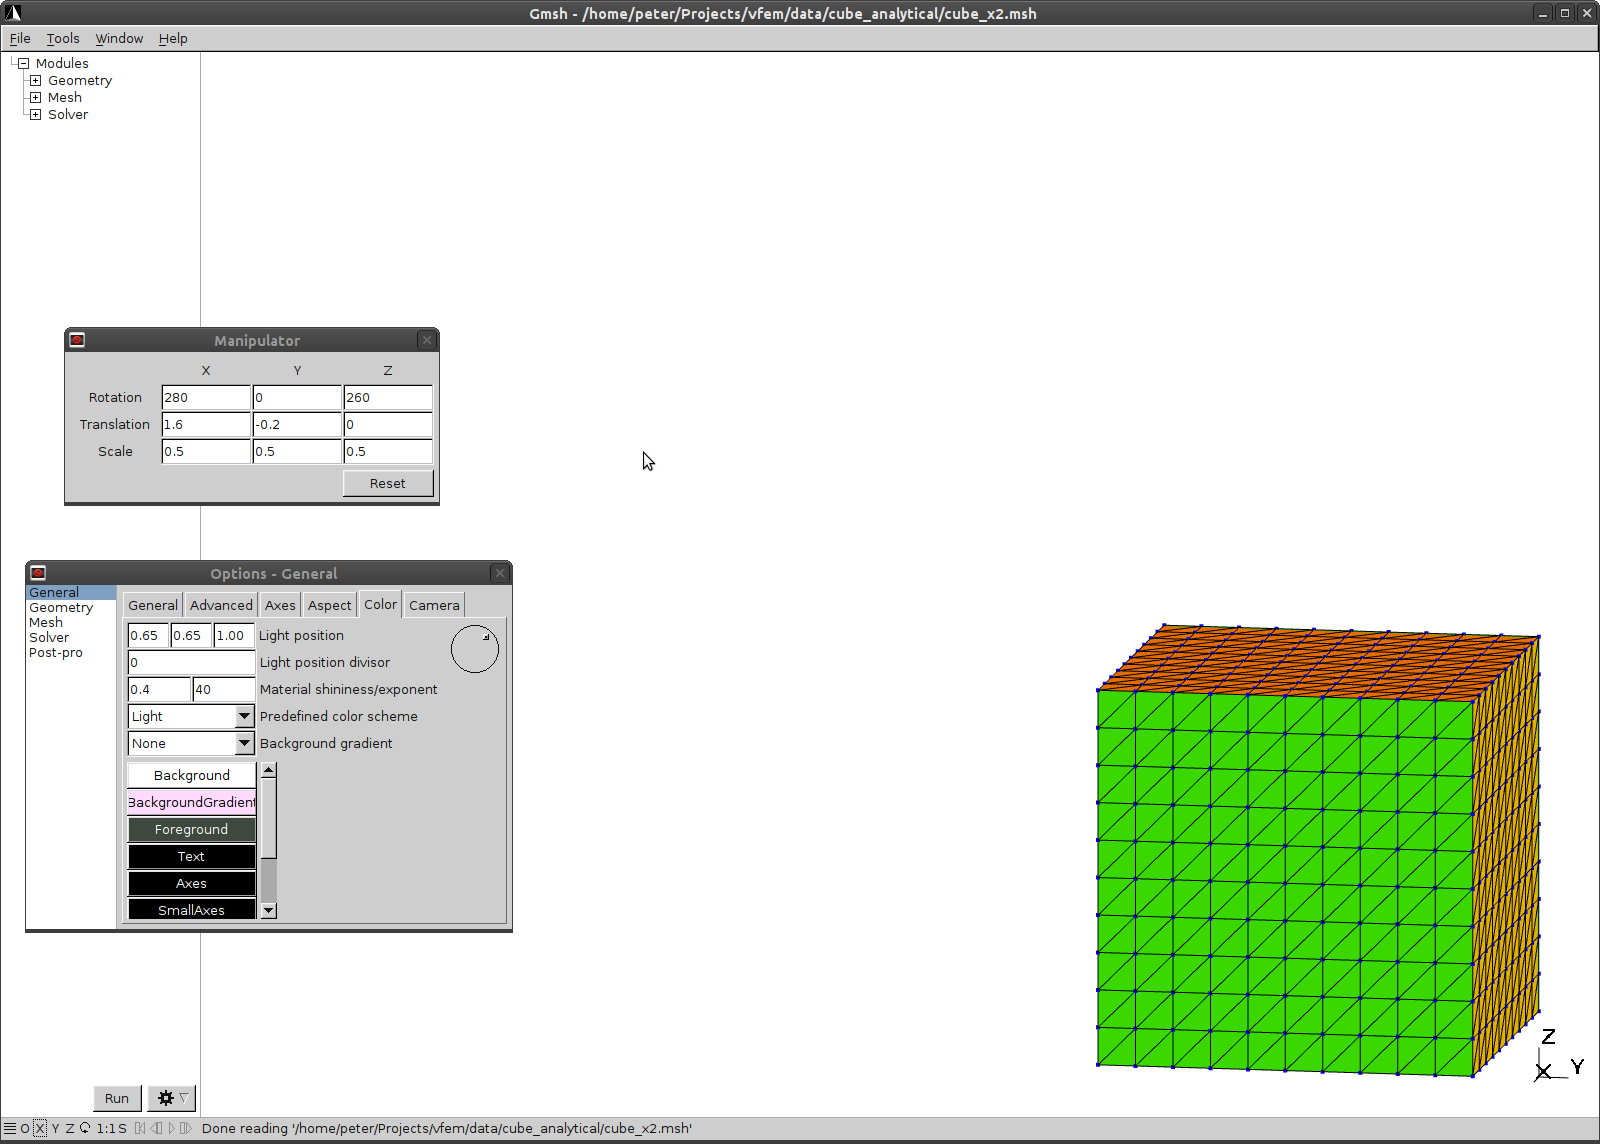
\includegraphics[trim=387mm 20mm 5mm 220mm,clip,scale=0.4]{verify/x2.png}\label{fig:verify:x2}}
	~~~~~
	\subfloat[][]{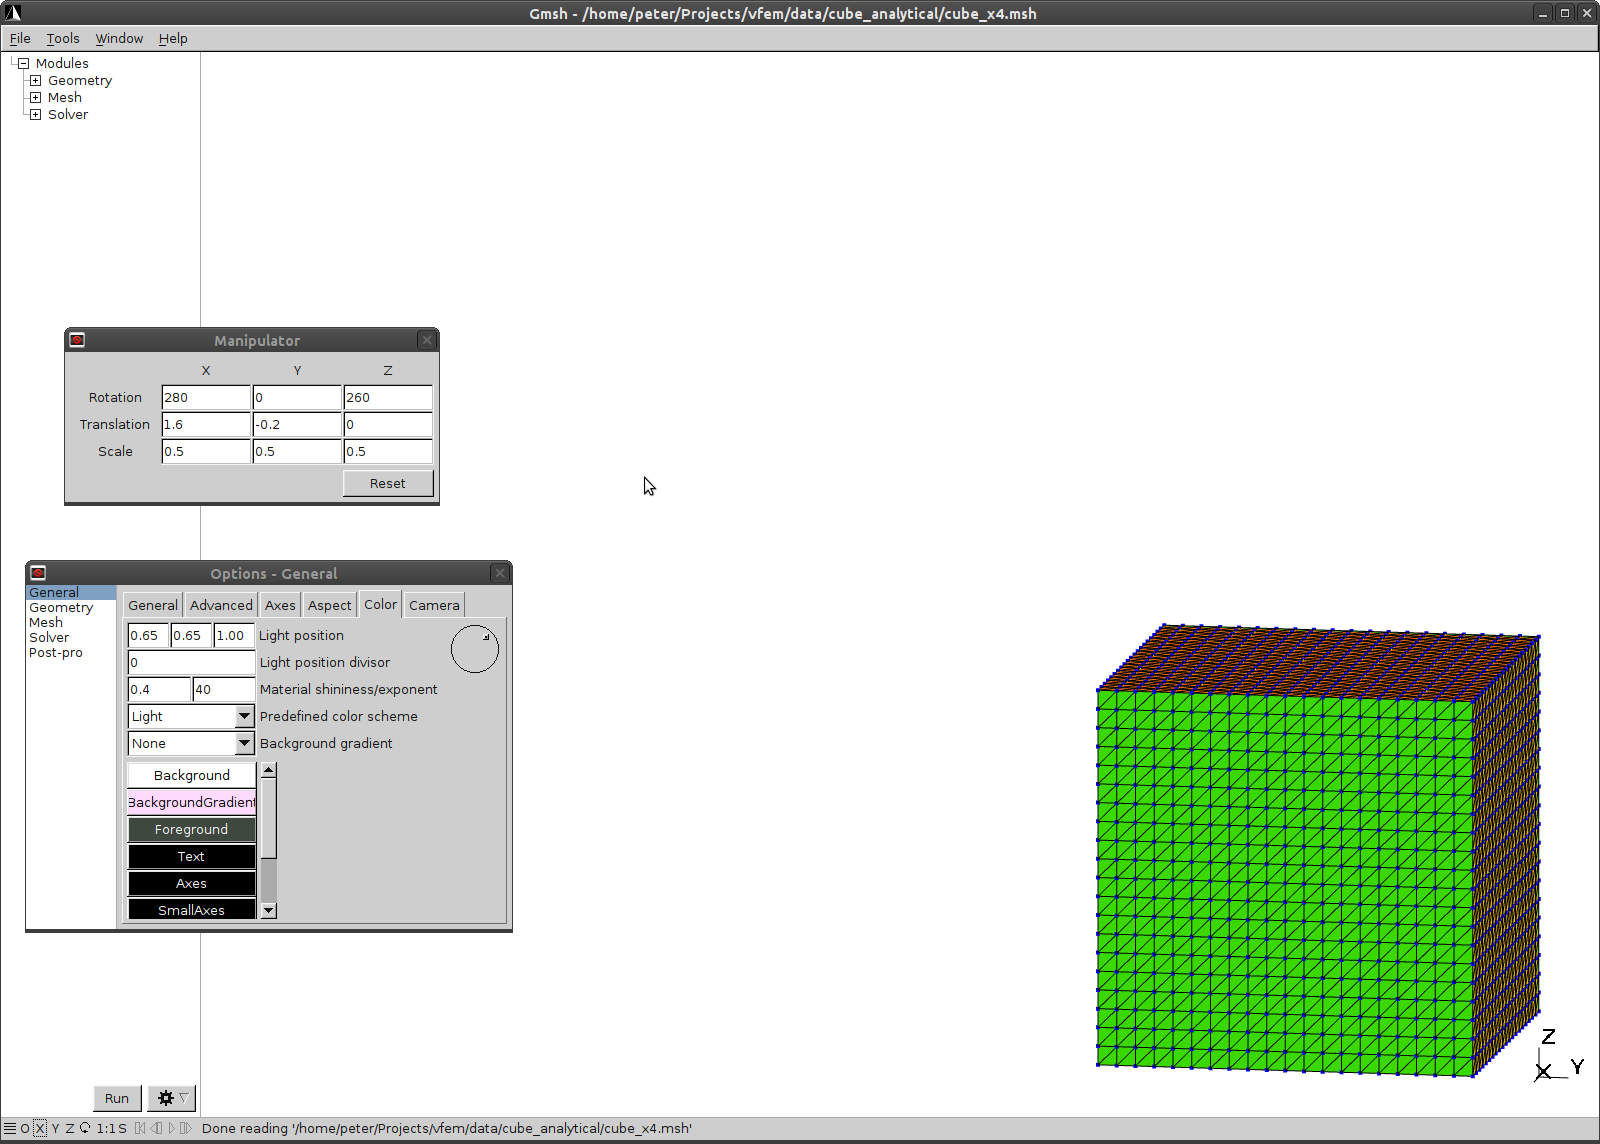
\includegraphics[trim=387mm 20mm 5mm 220mm,clip,scale=0.4]{verify/x4.png}\label{fig:verify:x4}}
	\caption{конечноэлементные сетки для определения порядка аппроксимации}
	\label{fig:verify:x2_x4}
\end{figure}

\begin{table}[H]
	\caption{относительные погрешности в норме $\mathbb{L}^2$}
	\label{tab:verify:exp_order}
	\begin{tabularx}{\textwidth}{|C{0.7}|C{0.9}|C{0.9}|C{0.9}|C{1.3}|C{1.3}|}
		\hline Порядок базиса &
		\raisebox{-0.7em}{$\smash{\frac{\| |\mathbf{E}| - |\mathbf{E}^{h}| \|_{\mathbb{L}^2}}{\| |\mathbf{E}| \|_{\mathbb{L}^2}}}$} &
		\raisebox{-0.7em}{$\smash{\frac{\| |\mathbf{E}| - |\mathbf{E}^{h/2}| \|_{\mathbb{L}^2}}{\| |\mathbf{E}| \|_{\mathbb{L}^2}}}$} &
		\raisebox{-0.7em}{$\smash{\frac{\| |\mathbf{E}| - |\mathbf{E}^{h/4}| \|_{\mathbb{L}^2}}{\| |\mathbf{E}| \|_{\mathbb{L}^2}}}$} &
		\raisebox{-0.7em}{$\smash{\log_2 \frac{\| |\mathbf{E}| - |\mathbf{E}^{h}| \|_{\mathbb{L}^2}}{\| |\mathbf{E}| - |\mathbf{E}^{h/2}| \|_{\mathbb{L}^2}}}$} &
		\raisebox{-0.7em}{$\smash{\log_2 \frac{\| |\mathbf{E}| - |\mathbf{E}^{h/2}| \|_{\mathbb{L}^2}}{\| |\mathbf{E}| - |\mathbf{E}^{h/4}| \|_{\mathbb{L}^2}}}$} \\
		\hline 1 & 6.608e-3 & 1.637e-3 & 5.051e-4 & 2.013 & 1.696 \\
		\hline 2 & 1.775e-4 & 2.164e-5 & 3.582e-6 & 3.036 & 2.595 \\
		\hline
	\end{tabularx}
\end{table}
\vspace{-0.5cm}

Из результатов видно, что порядок аппроксимации получился второй для базисных функций первого порядка и третий для базисных функций второго порядка, что совпадает с теоретическими значениями.

% =============================================================================

\clearpage
\section{Вычислительные эксперименты}
\subsection{Исследование влияния слоя воздуха}

Проведем исследование влияния слоя воздуха в модельной задаче морской геоэлектрики при различной глубине погружения в воду источника электромагнитного возмущения.

В этом исследовании будем пользоваться базисными функциями второго полного порядка.

\subsubsection{Описание расчетной области}
Схематичное изображение расчетной области показано на рисунке \ref{fig:res1:area}, где $\Omega_1$ -- воздух ($\sigma=10^{-6}$ См/м, $\mu=\mu_0$, $\varepsilon=\varepsilon_0$); $\Omega_2$ -- морская вода ($\sigma=3.3$ См/м, $\mu=\mu_0$, $\varepsilon=\varepsilon_0$); $\Omega_3$ -- грунт ($\sigma=0.2$ См/м, $\mu=\mu_0$, $\varepsilon=\varepsilon_0$); $\Omega_4$ -- углеводороды ($\sigma=10^{-2}$~См/м, $\mu=\mu_0$, $\varepsilon=\varepsilon_0$); $L_1$, $L_2$ и $L_3$ -- размеры области моделирования по осям $x$, $y$ и $z$ соответственно; $L_1 = L_2 = L_3 = 6000$~м; $h_1=600$~м -- толщина $\Omega_2$; $l_1=400$~м, $h_3=75$~м, $h_2=135$~м -- длина, толщина и глубина объекта $\Omega_4$ соответственно.

\begin{figure}[H]
	\centering
	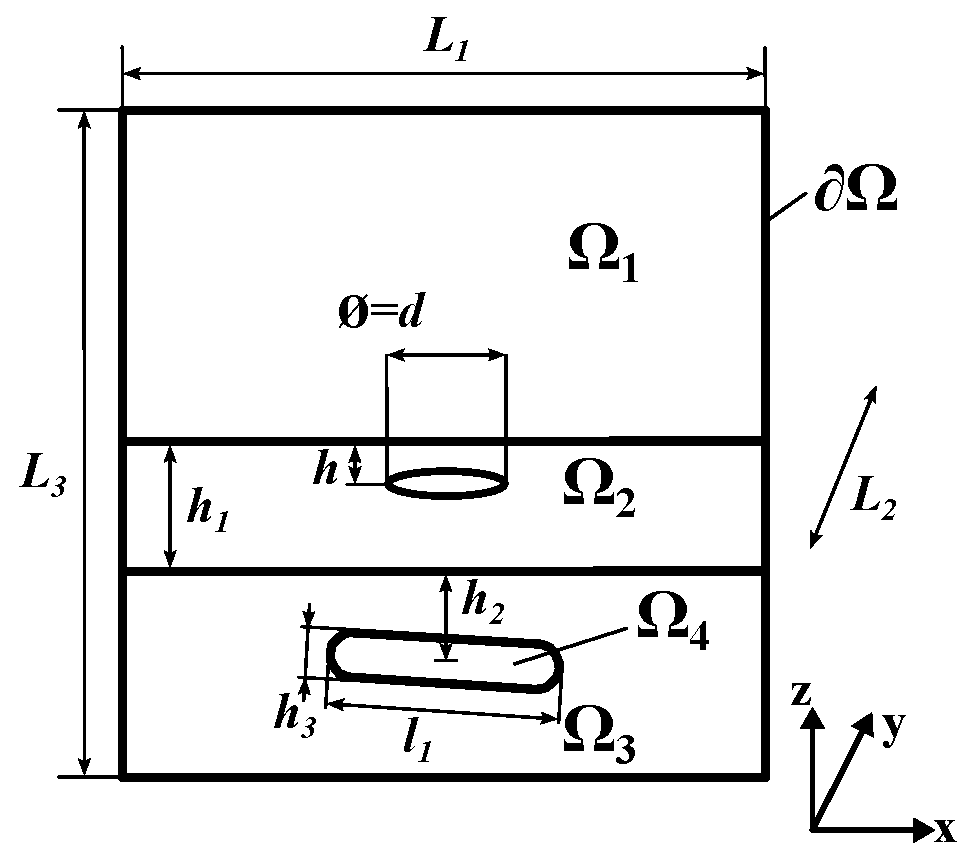
\includegraphics[scale=0.7]{research-1/area_3layers_shift_3.eps}
	\caption{схематичное изображение расчетной области}
	\label{fig:res1:area}
\end{figure}

\noindent Объект $\Omega_4$ представляет собой скругленный прямоугольный параллелепипед с двумя равными сторонами, наклоненный под углом $5^{\circ}$. Источником электрического поля является токовая петля диаметром $d=100$~м с током частотой 1~Гц, глубина $h$ которой варьируется в ходе исследования.

\subsubsection{Конечноэлементная сетка}
Фрагмент $x \in [-600,0]$, $y \in [-600,600]$ $z \in [-1000,600]$ одной из конечноэлементных сеток, использованных для проведения исследования, представлен на рисунке \ref{fig:res1:mesh}.

\begin{figure}[H]
	\centering
	% trim=left bottom right top
	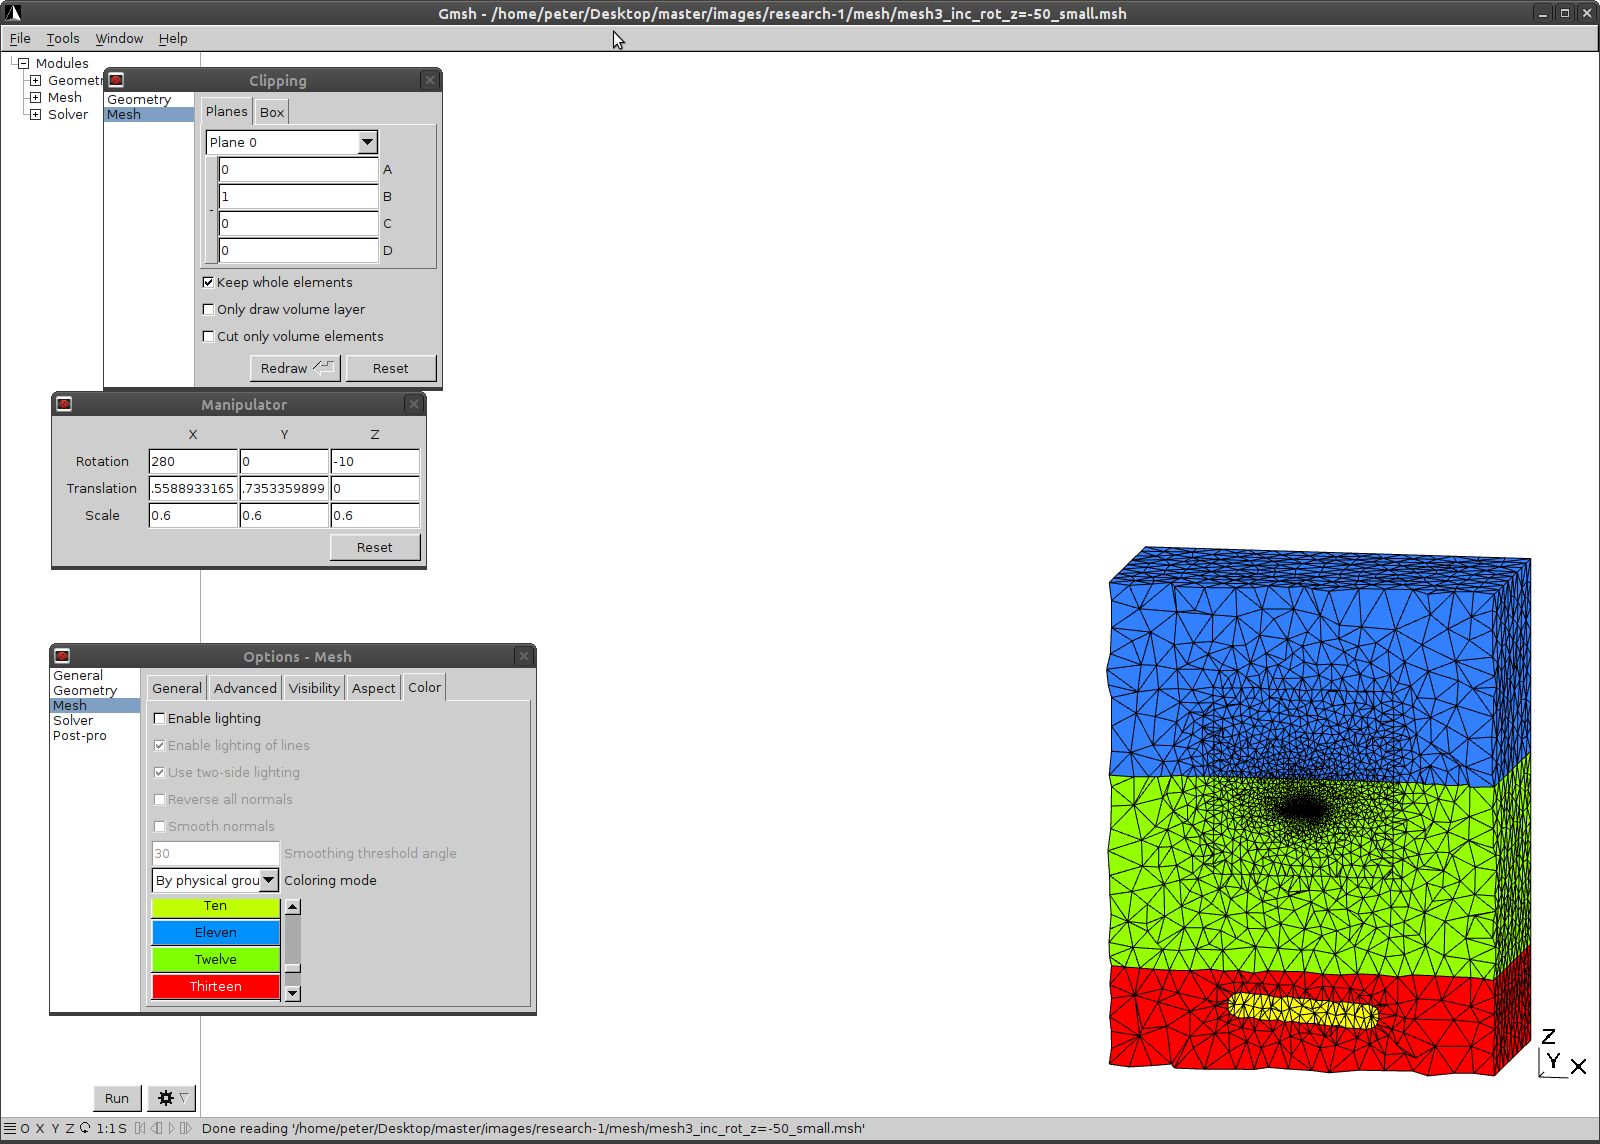
\includegraphics[trim=390mm 20mm 5mm 195mm,clip,scale=0.5]{research-1/mesh/mesh.png}
	\caption{фрагмент конечноэлементной сетки}
	\label{fig:res1:mesh}
\end{figure}

\subsubsection{Результаты исследования}
Разности решений в норме $\mathbb{L}^2$ в объеме $[-600,600] \times [-600,600] \times [-1000,0]$ между областью, в которой присутствует слой воздуха, и областью, в которой заданы условия непротекания~(\ref{eq:bound2}), для некоторых значений глубины петли $h$ показаны в таблице \ref{tab:res1:diff}. В форме графика эти данные приведены на рисунке \ref{fig:res1:graph}.

\begin{table}[H]
	\caption{относительные разности решений}
	\label{tab:res1:diff}
	\begin{tabularx}{\textwidth}{|C{2.4}|C{0.8}|C{0.8}|C{0.8}|C{0.8}|C{0.8}|C{0.8}|C{0.8}|}
		\hline Глубина петли & 5 & 10 & 50 & 100 & 200 & 300 & 400 \\
		\hline $\displaystyle \frac{\| | \mathbf{E}^{air} - \mathbf{E}^{noair} | \|_{\mathbb{L}^2}}{\| | \mathbf{E}^{air} | \|_{\mathbb{L}^2}}$ & 0.44 & 0.40 & 0.24 & 0.14 & 0.07 & 0.04 & 0.02 \\
		\hline
	\end{tabularx}
\end{table}

\begin{figure}[H]
	\centering
	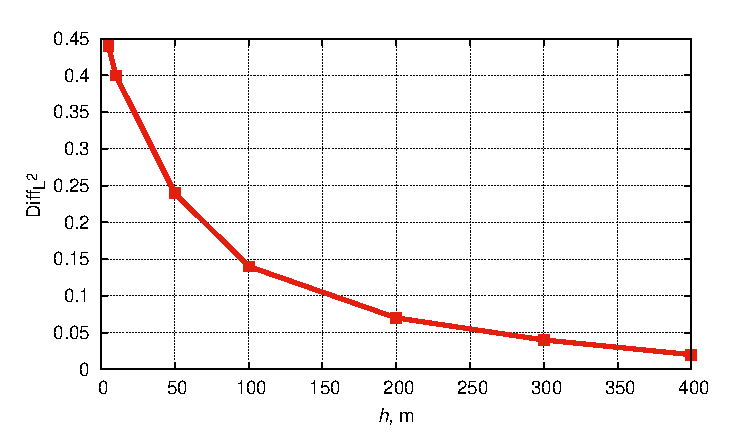
\includegraphics[scale=1]{research-1/presentation/presentation.eps}
	\caption{график изменения относительной разности решений при изменении глубины}
	\label{fig:res1:graph}
\end{figure}

Графики вещественной компоненты $\mathbf{E}_y$ по линии $y=0$, $z=-610$ для различных глубин петли представлены на рисунках \ref{fig:res1:5_50} и \ref{fig:res1:200_300}.

\begin{figure}[H]
	\centering
	\subfloat[][]{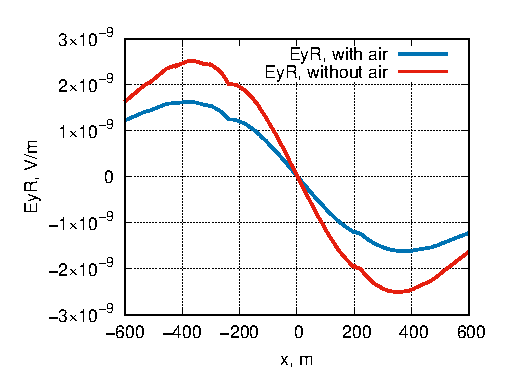
\includegraphics[scale=1]{research-1/-5/EyR_-700.eps}\label{fig:res1:5}}
	~
	\subfloat[][]{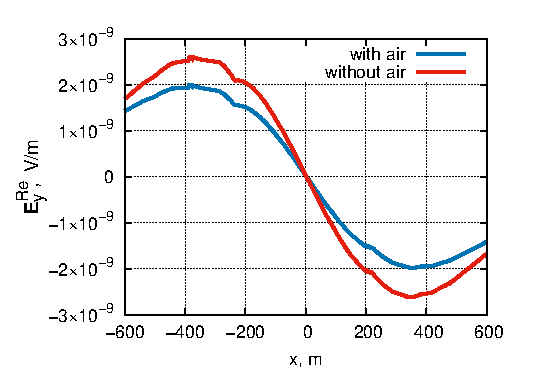
\includegraphics[scale=1]{research-1/-50/EyR_-700.eps}\label{fig:res1:50}}
	\caption{$\Re(\mathbf{E}_y)$ по линии $y=0$, $z=-610$, глубина (а) 5 м и (б) 50 м}
	\label{fig:res1:5_50}
\end{figure}

\begin{figure}[H]
	\centering
	\subfloat[][]{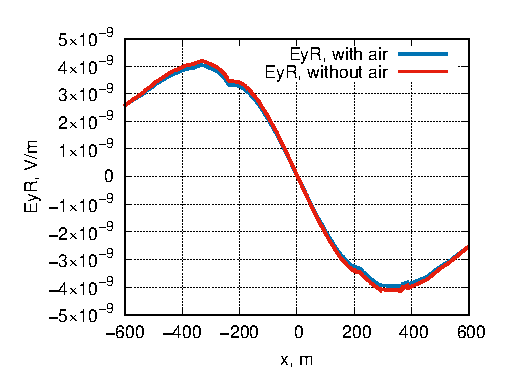
\includegraphics[scale=1]{research-1/-200/EyR_-700.eps}\label{fig:res1:200}}
	~
	\subfloat[][]{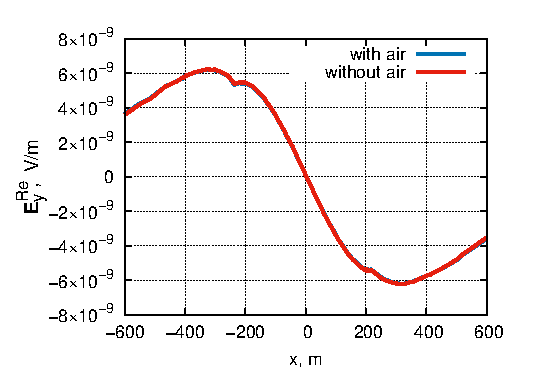
\includegraphics[scale=1]{research-1/-300/EyR_-700.eps}\label{fig:res1:300}}
	\caption{$\Re(\mathbf{E}_y)$ по линии $y=0$, $z=-610$, глубина (а) 200 м и (б) 300 м}
	\label{fig:res1:200_300}
\end{figure}

Из результатов следует, что слой воздуха оказывает значительное влияние на получаемое решение при расположении источника электромагнитного возмущения на малой глубине (меньше трехсот метров для рассмотренной конфигурации).

% =============================================================================

\subsection{Исследование эффективности применения PML-слоя}
Цель вычислительных экспериментов: определение эффективности применения PML-слоя. Геометрические характеристики PML-слоя показаны на рисунке \ref{fig:res2:info_2d}.
\begin{figure}[H]
	\centering
	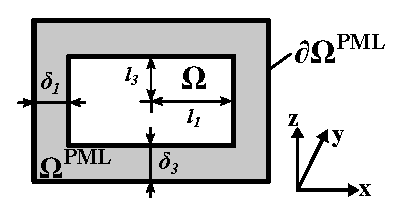
\includegraphics[scale=1.25]{research-2/info_2d/info_2d_2.eps}
	\caption{геометрические характеристики PML-слоя}
	\label{fig:res2:info_2d}
\end{figure}

Вычислительные эксперименты проводились следующим образом: последовательно варьировался каждый из параметров PML-слоя: толщина слоя в $k$-м направлении $\delta_k$, где $k = \begin{smallmatrix}x\\1\end{smallmatrix},\begin{smallmatrix}y\\2\end{smallmatrix},\begin{smallmatrix}z\\3\end{smallmatrix}$, расстояние от центра области до внутренних границ слоя $l_k$, коэффициент комплексного растяжения координат $\chi$~(\ref{eq:pml_s}), оставшиеся параметры фиксировались, что позволило определить параметры, оказывающие наибольшее влияние на характеристики PML-слоя.

Фрагменты тетраэдральных конечноэлементных сеток с <<большим баком>> и с PML-слоем приведены на рисунках \ref{fig:res2:meshes_a} и \ref{fig:res2:meshes_b}.
\begin{figure}[H]
	\centering
	% trim=left bottom right top
	\subfloat[][]{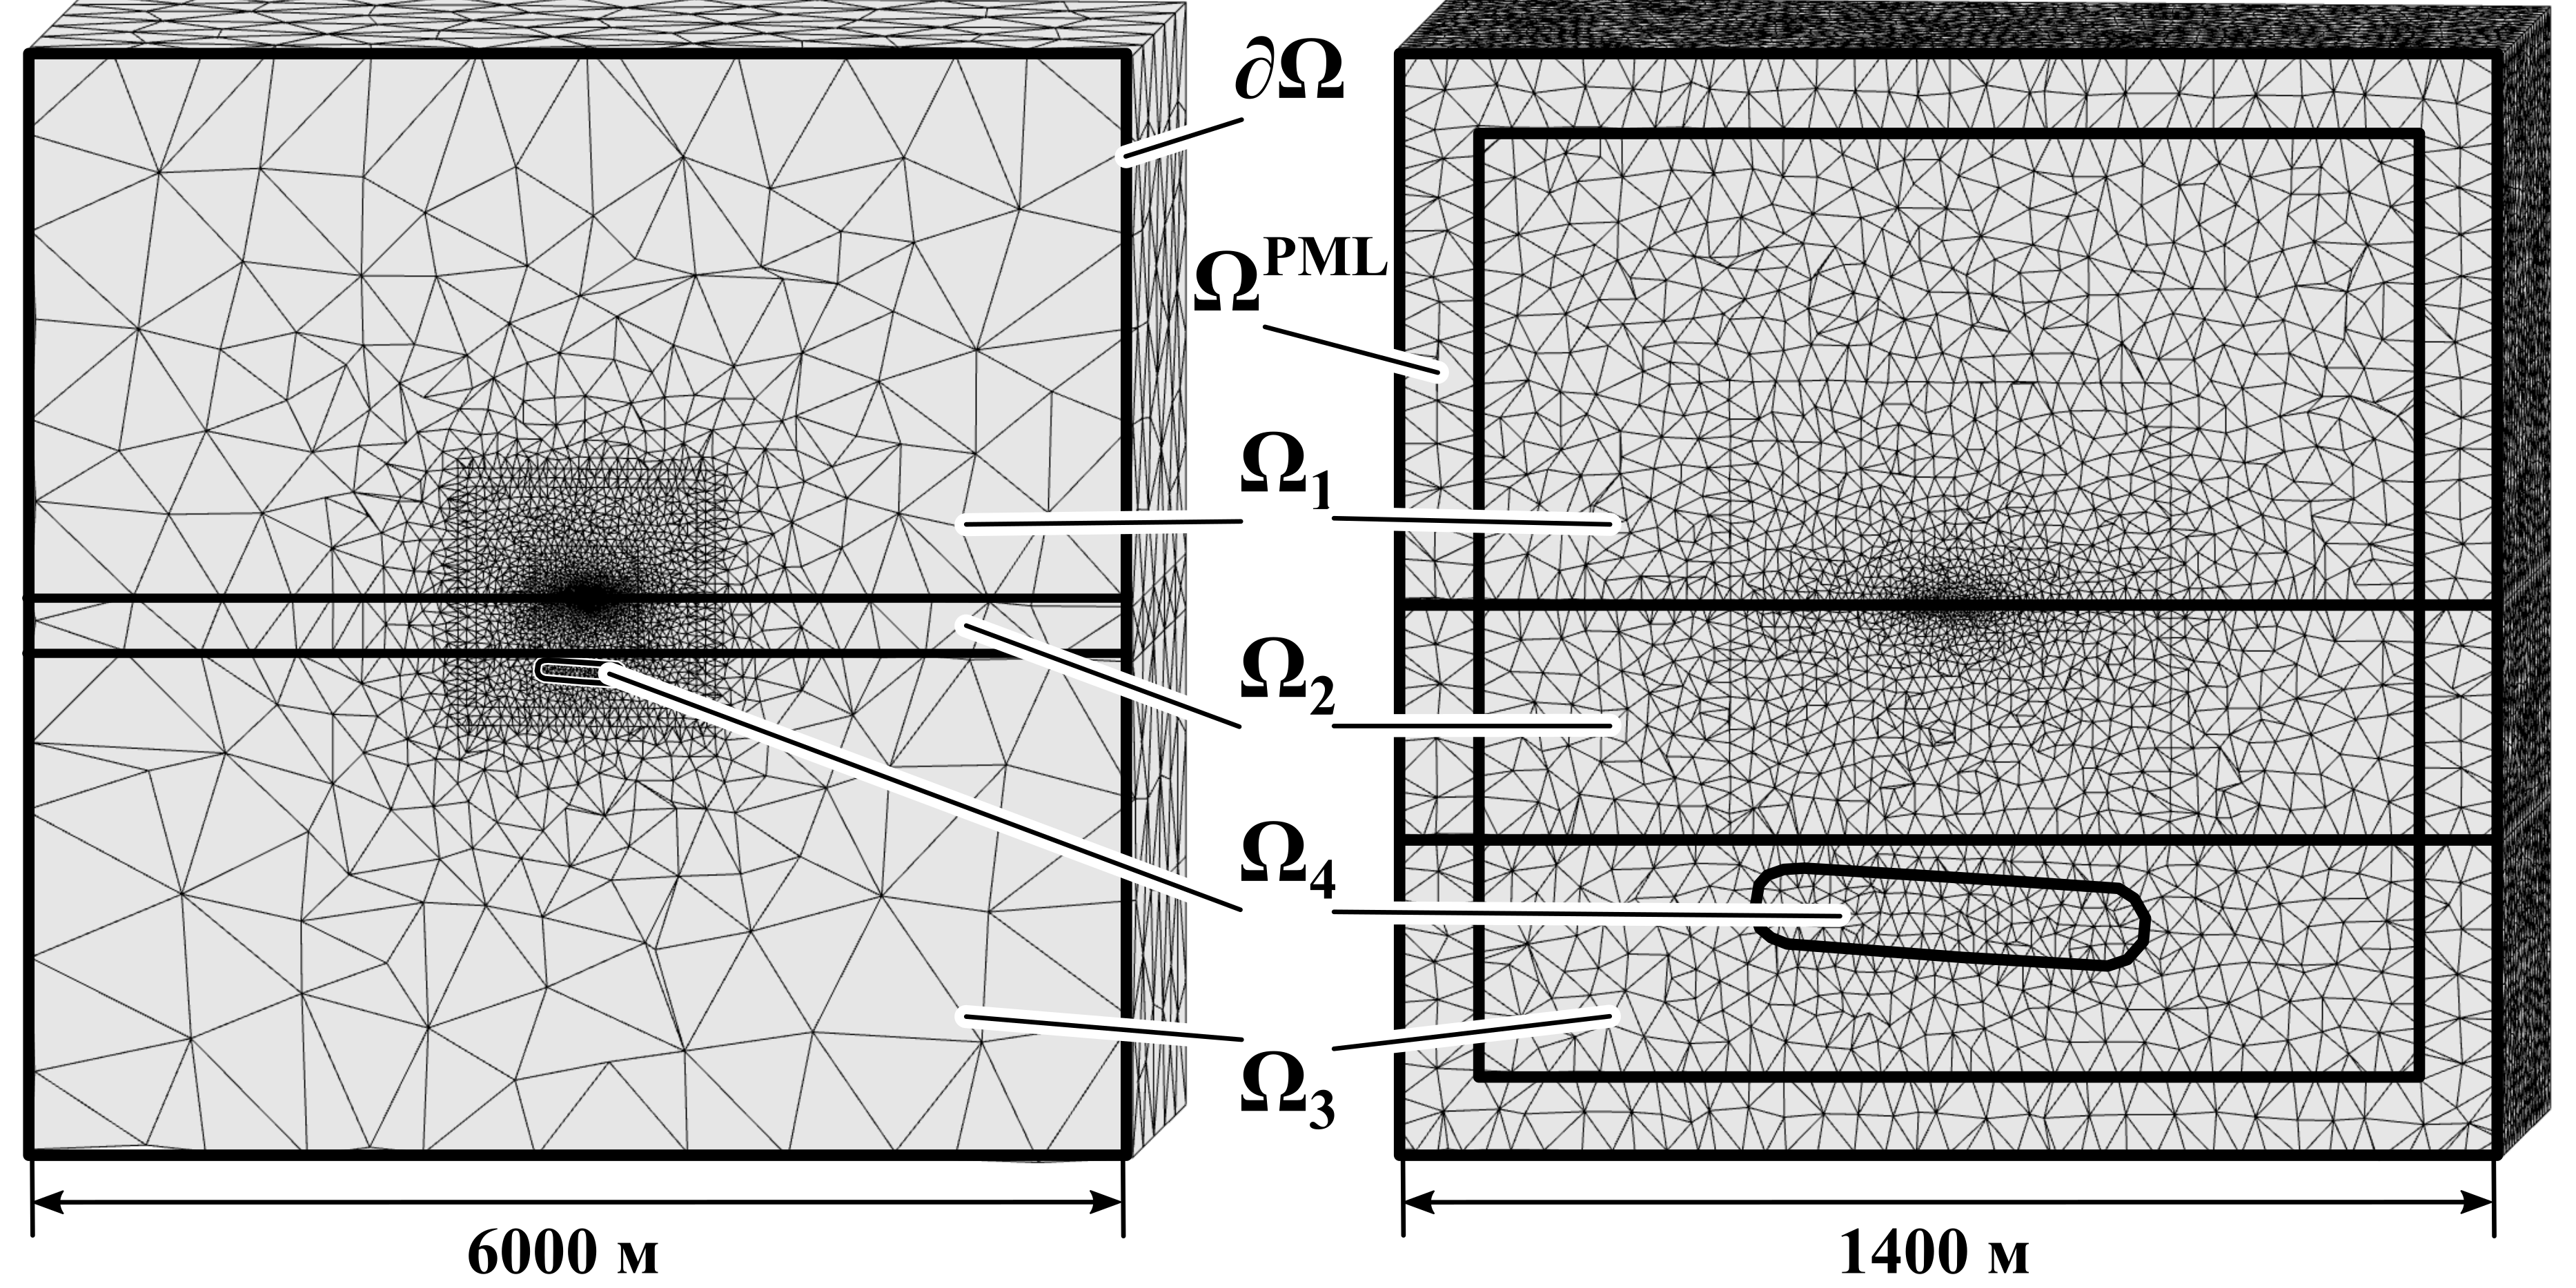
\includegraphics[trim=0mm 0mm 79.2mm 0mm,clip,scale=1.1]{research-2/meshes/meshes.png}\label{fig:res2:meshes_a}}
	\subfloat[][]{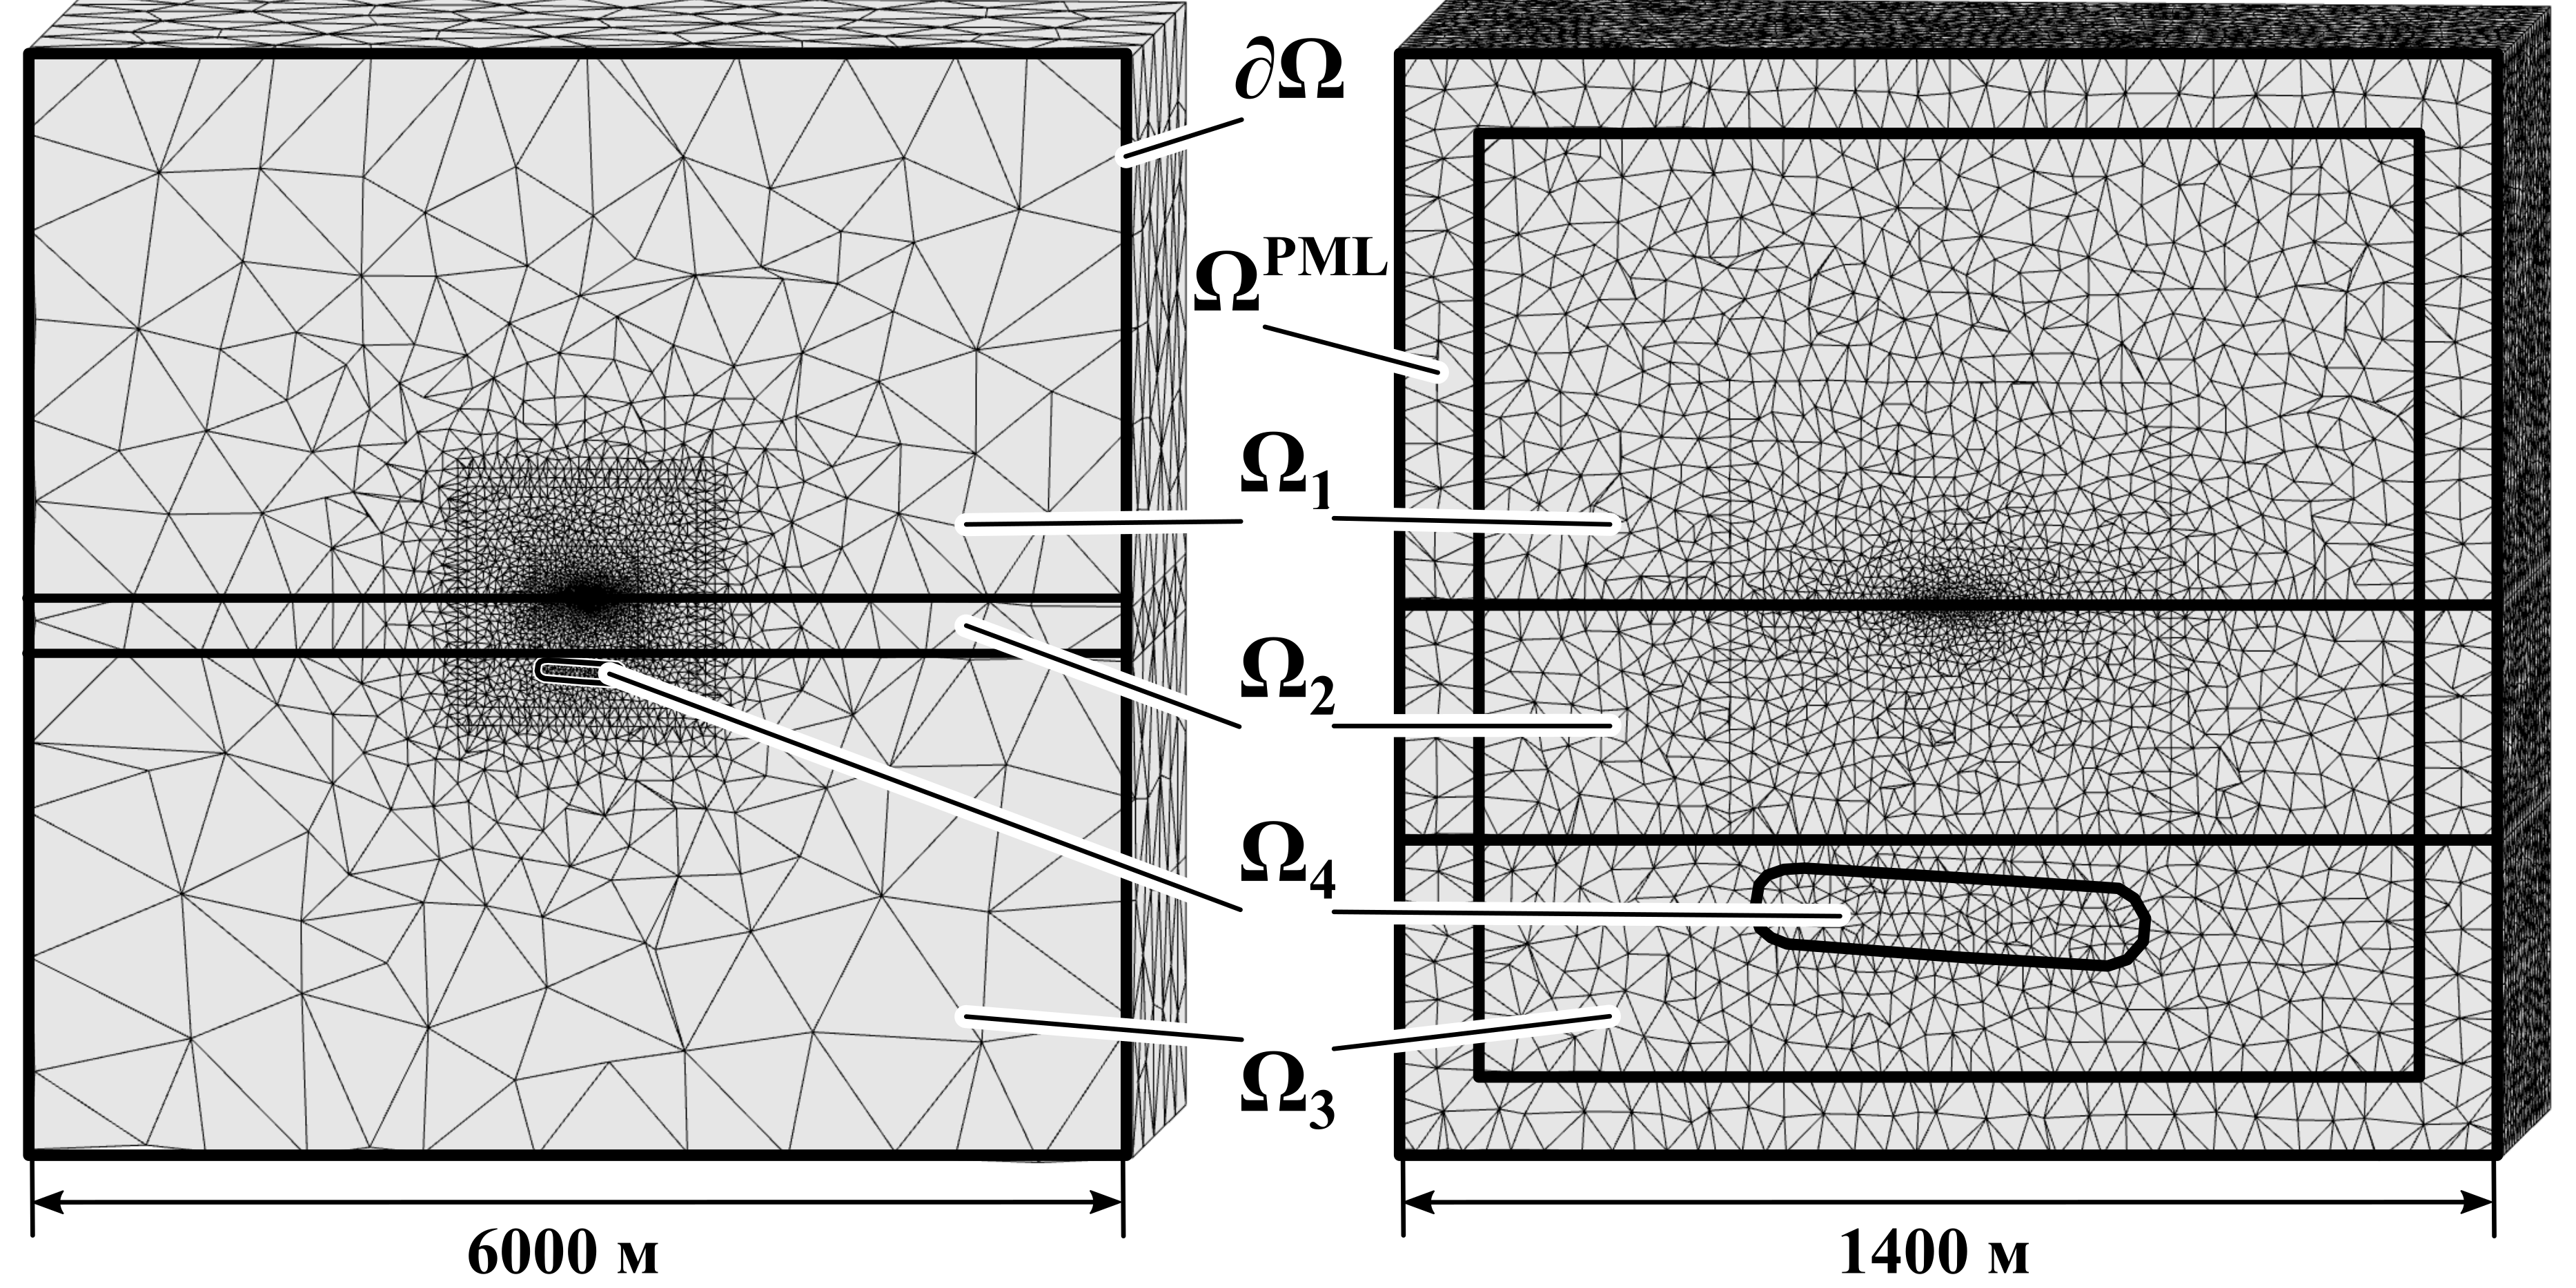
\includegraphics[trim=78.8mm 0mm 0mm 0mm,clip,scale=1.1]{research-2/meshes/meshes.png}\label{fig:res2:meshes_b}}
	\caption{конечноэлементные сетки: (а) <<большой бак>> и (б) PML-слой}
	\label{fig:res2:meshes}
\end{figure}

В этом исследовании будем пользоваться базисными функциями первого полного порядка.

\subsubsection{Описание расчетной области}
Схематичное изображение расчетной области показано на рисунке \ref{fig:res2:area}, где $\Omega_1$ -- воздух ($\sigma=10^{-6}$ См/м, $\mu=\mu_0$, $\varepsilon=\varepsilon_0$); $\Omega_2$ -- морская вода ($\sigma=3.3$ См/м, $\mu=\mu_0$, $\varepsilon=\varepsilon_0$); $\Omega_3$ -- грунт ($\sigma=0.2$ См/м, $\mu=\mu_0$, $\varepsilon=\varepsilon_0$); $\Omega_4$ -- углеводороды ($\sigma=10^{-2}$~См/м, $\mu=\mu_0$, $\varepsilon=\varepsilon_0$); $L_1$, $L_2$ и $L_3$ -- размеры области моделирования по осям $x$, $y$ и $z$ соответственно; $L_1 = L_2 = L_3 = 6000$~м; $h_1=300$~м -- толщина $\Omega_2$; $l_1=400$~м, $h_3=100$~м, $h_2=100$~м -- длина, толщина и глубина объекта $\Omega_4$ соответственно.

Объект $\Omega_4$ представляет собой скругленный прямоугольный параллелепипед с двумя равными сторонами, наклоненный под углом $5^{\circ}$. Источником электрического поля является петля диаметром $d = 100$~м с током частотой $1$~Гц, расположенная в воздухе на расстоянии $h = 5$~м от границы раздела сред воздух-вода. Также рассматривается случай, когда петля расположена в воде ($h = -5$~м).

\begin{figure}[H]
	\centering
	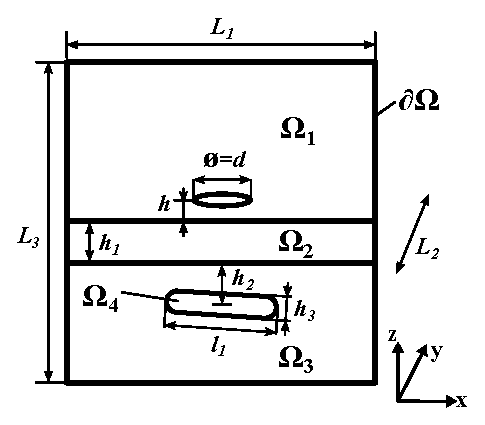
\includegraphics[scale=1.5]{research-2/area_3layers/area_3layers_3.eps}
	\caption{расчетная область}
	\label{fig:res2:area}
\end{figure}

Выделим внутри области c условием <<большого бака>> и области, на границе которой задан PML-слой, подобласть $\Omega'$ размером $1000 \times 1000 \times 1000$~м${}^3$. Для этой подобласти в данном исследовании будем оценивать разность в норме $\mathbb{L}^2$ между действительными компонентами $\mathbf{E}_y$ векторов решений $\mathbf{E}_y^{\text{бак}}$ и $\mathbf{E}_y^{\text{PML}}$, полученных с применением <<большого бака>> и PML-слоя соответственно.

\subsubsection{Варьирование коэффициентов растяжения}
Зафиксируем $\delta_k = 100$~м, $l_k = 600$~м, $m = 3$, $h = 5$~м и будем варьировать коэффициент комплексного растяжения координат $\chi$. Размер получаемой СЛАУ для <<большого бака>> -- 653814, с PML-слоем -- 616180. Результаты приведены в таблице \ref{tab:res2:chi_5}. Для случая $h= -5$~м размер получаемой СЛАУ для <<большого бака>> -- 652396, с PML-слоем -- 614504. Результаты приведены в таблице \ref{tab:res2:chi_m5}.
\begin{table}[H]
	\caption{варьирование коэффициентов растяжения при $h= 5$~м}
	\label{tab:res2:chi_5}
	\begin{spacing}{1.2}
	\setlength{\parskip}{0pt}
	\fontsize{12}{14}\selectfont
	\begin{tabularx}{\textwidth}{|C{0.65}|C{0.65}|C{0.65}|C{0.65}|C{0.65}|C{0.65}|C{3.1}|C{1}|C{1}|}
		\rowcolor[gray]{.9} \hline $\Re(\chi)$ в $\Omega_1$ & $\Im(\chi)$ в $\Omega_1$ & $\Re(\chi)$ в $\Omega_2$ & $\Im(\chi)$ в $\Omega_2$ & $\Re(\chi)$ в $\Omega_3$ & $\Im(\chi)$ в $\Omega_3$ & \raisebox{-0.8em}{$\smash{\displaystyle \frac{\lVert \Re(\mathbf{E}_y^{\text{бак}}) - \Re(\mathbf{E}_y^{\text{PML}})\rVert}{\lVert \Re(\mathbf{E}_y^{\text{бак}})\rVert}}$} & Время, бак & Время, PML \\[0.2em]
		\hline 3 & 0 & 1 & 5 & 3 & 1 & 0.106636 & \multirow{4}{*}{650} & 592 \\
		\cline{1-7}\cline{9-9} 3 & 1 & 0 & 6 & 2 & 1 & 0.0925 & & 599 \\
		\cline{1-7}\cline{9-9} 4 & 0 & 1 & 5 & 3 & 1 & 0.0947 & & 731 \\
		\cline{1-7}\cline{9-9} 4 & 1 & 0 & 6 & 2 & 1 & 0.0910 & & 591 \\
		\hline
	\end{tabularx}
	\end{spacing}
\end{table}

\begin{table}[H]
	\caption{варьирование коэффициентов растяжения при $h= -5$~м}
	\label{tab:res2:chi_m5}
	\begin{spacing}{1.2}
	\setlength{\parskip}{0pt}
	\fontsize{12}{14}\selectfont
	\begin{tabularx}{\textwidth}{|C{0.65}|C{0.65}|C{0.65}|C{0.65}|C{0.65}|C{0.65}|C{3.1}|C{1}|C{1}|}
		\rowcolor[gray]{.9} \hline $\Re(\chi)$ в $\Omega_1$ & $\Im(\chi)$ в $\Omega_1$ & $\Re(\chi)$ в $\Omega_2$ & $\Im(\chi)$ в $\Omega_2$ & $\Re(\chi)$ в $\Omega_3$ & $\Im(\chi)$ в $\Omega_3$ & \raisebox{-0.8em}{$\smash{\displaystyle \frac{\lVert \Re(\mathbf{E}_y^{\text{бак}}) - \Re(\mathbf{E}_y^{\text{PML}})\rVert}{\lVert \Re(\mathbf{E}_y^{\text{бак}})\rVert}}$} & Время, бак & Время, PML \\[0.2em]
		\hline 4 & 0 & 1 & 5 & 3 & 1 & 0.0929047 & \multirow{4}{*}{309} & 344 \\
		\cline{1-7}\cline{9-9} 4 & 0 & 1 & 6 & 3 & 1 & 0.0870 & & 294 \\
		\cline{1-7}\cline{9-9} 4 & 0 & 1 & 6 & 3 & 2 & 0.0809 & & 253 \\
		\cline{1-7}\cline{9-9} 4 & 1 & 1 & 6 & 3 & 2 & 0.0658 & & 306 \\
		\hline
	\end{tabularx}
	\end{spacing}
\end{table}

\subsubsection{Варьирование толщины PML-слоя}
Зафиксируем $\chi_{\Omega_1} = (4, 1)$, $\chi_{\Omega_2} = (0, 6)$, $\chi_{\Omega_3} = (2, 1)$, $l_k = 600$~м, $m = 3$, $h = 5$~м и будем варьировать толщину PML-слоя $\delta_k$. Результаты приведены в таблице \ref{tab:res2:delta_5}. Для случая $h= -5$~м выберем $\chi_{\Omega_1} = (4, 0)$, $\chi_{\Omega_2} = (1, 6)$, $\chi_{\Omega_3} = (3, 2)$. Результаты приведены в таблице \ref{tab:res2:delta_m5}.

\begin{table}[H]
	\caption{варьирование толщины PML-слоя при $h= 5$~м}
	\label{tab:res2:delta_5}
	\begin{spacing}{1.2}
	\setlength{\parskip}{0pt}
	\fontsize{12}{14}\selectfont
	\begin{tabularx}{\textwidth}{|C{0.4}|C{2.2}|C{0.8}|C{0.8}|C{0.9}|C{0.9}|}
		\rowcolor[gray]{.9} \hline \raisebox{-0.8em}[0.8em]{$\smash{\displaystyle \delta_k}$} & \raisebox{-0.8em}[0.8em]{$\smash{\displaystyle \frac{\lVert \Re(\mathbf{E}_y^{\text{бак}}) - \Re(\mathbf{E}_y^{\text{PML}})\rVert}{\lVert \Re(\mathbf{E}_y^{\text{бак}})\rVert}}$} & Время, бак & Время, PML & Размер СЛАУ, бак & Размер СЛАУ, PML \\[0.2em]
		\hline 80 & 0.1199 & 673 & 1289 & 659858 & 618128 \\
		\hline 100 & 0.0910 & 650 & 591 & 653814 & 616180 \\
		\hline 120 & 0.0784 & 609 & 1142 & 654354 & 617324 \\
		\hline
	\end{tabularx}
	\end{spacing}
\end{table}

\begin{table}[H]
	\caption{варьирование толщины PML-слоя при $h= -5$~м}
	\label{tab:res2:delta_m5}
	\begin{spacing}{1.2}
	\setlength{\parskip}{0pt}
	\fontsize{12}{14}\selectfont
	\begin{tabularx}{\textwidth}{|C{0.4}|C{2.2}|C{0.8}|C{0.8}|C{0.9}|C{0.9}|}
		\rowcolor[gray]{.9} \hline \raisebox{-0.8em}[0.8em]{$\smash{\displaystyle \delta_k}$} & \raisebox{-0.8em}[0.8em]{$\smash{\displaystyle \frac{\lVert \Re(\mathbf{E}_y^{\text{бак}}) - \Re(\mathbf{E}_y^{\text{PML}})\rVert}{\lVert \Re(\mathbf{E}_y^{\text{бак}})\rVert}}$} & Время, бак & Время, PML & Размер СЛАУ, бак & Размер СЛАУ, PML \\[0.2em]
		\hline 80 & 0.1201 & 359 & 297 & 652312 & 614822 \\
		\hline 100 & 0.0809 & 309 & 253 & 652396 & 614504 \\
		\hline 120 & 0.0623 & 250 & 859 & 652422 & 615394\\
		\hline
	\end{tabularx}
	\end{spacing}
\end{table}

\subsubsection{Варьирование размера области, на границе которой вводится PML-слой}
Зафиксируем $\chi_{\Omega_1} = (4, 1)$, $\chi_{\Omega_2} = (0, 6)$, $\chi_{\Omega_3} = (2, 1)$, $\delta_k = 100$~м, $m = 3$, $h = 5$~м и будем варьировать $l_k$ -- размер области, на границе которой вводится PML-слой. Результаты приведены в таблице \ref{tab:res2:l_5}. Для случая $h= -5$~м выберем $\chi_{\Omega_1} = (4, 0)$, $\chi_{\Omega_2} = (1, 6)$, $\chi_{\Omega_3} = (3, 2)$. Результаты приведены в таблице \ref{tab:res2:l_m5}.

\begin{table}[H]
	\caption{варьирование размера области, на границе которой вводится PML-слой, при $h= 5$~м}
	\label{tab:res2:l_5}
	\begin{spacing}{1.2}
	\setlength{\parskip}{0pt}
	\fontsize{12}{14}\selectfont
	\begin{tabularx}{\textwidth}{|C{0.4}|C{2.2}|C{0.8}|C{0.8}|C{0.9}|C{0.9}|}
		\rowcolor[gray]{.9} \hline \raisebox{-0.8em}[0.8em]{$\smash{\displaystyle l_k}$} & \raisebox{-0.8em}[0.8em]{$\smash{\displaystyle \frac{\lVert \Re(\mathbf{E}_y^{\text{бак}}) - \Re(\mathbf{E}_y^{\text{PML}})\rVert}{\lVert \Re(\mathbf{E}_y^{\text{бак}})\rVert}}$} & Время, бак & Время, PML & Размер СЛАУ, бак & Размер СЛАУ, PML \\[0.2em]
		\hline 500 & 0.187456 & 628 & 587 & 659130 & 621390 \\
		\hline 600 & 0.0909998 & 650 & 591 & 652396 & 614504 \\
		\hline 800 & 0.0440642 & 718 & 658 & 794310 & 744856 \\
		\hline
	\end{tabularx}
	\end{spacing}
\end{table}

\begin{table}[H]
	\caption{варьирование размера области, на границе которой вводится PML-слой, при $h= -5$~м}
	\label{tab:res2:l_m5}
	\begin{spacing}{1.2}
	\setlength{\parskip}{0pt}
	\fontsize{12}{14}\selectfont
	\begin{tabularx}{\textwidth}{|C{0.4}|C{2.2}|C{0.8}|C{0.8}|C{0.9}|C{0.9}|}
		\rowcolor[gray]{.9} \hline \raisebox{-0.8em}[0.8em]{$\smash{\displaystyle l_k}$} & \raisebox{-0.8em}[0.8em]{$\smash{\displaystyle \frac{\lVert \Re(\mathbf{E}_y^{\text{бак}}) - \Re(\mathbf{E}_y^{\text{PML}})\rVert}{\lVert \Re(\mathbf{E}_y^{\text{бак}})\rVert}}$} & Время, бак & Время, PML & Размер СЛАУ, бак & Размер СЛАУ, PML \\[0.2em]
		\hline 500 & 0.1751746 & 317 & 238 & 659814 & 621390 \\
		\hline 600 & 0.0809429 & 309 & 253 & 652396 & 614504 \\
		\hline 800 & 0.0348019 & 357 & 329 & 793272 & 743780 \\
		\hline
	\end{tabularx}
	\end{spacing}
\end{table}

\subsubsection{Проверка выполнения условий на контактных границах}
Проверим, что в случае независимого варьирования коэффициентов комплексного растяжения координат $\chi$, на границе двух соседних PML-слоев с различными характеристиками не нарушаются условия на контактных границах (\ref{eq:maxwell:tangent_E})-(\ref{eq:maxwell:normal_D}). Для этого рассмотрим напряженность электрического поля $\mathbf{E}$ вдоль линии $x = 650$, $y = 0$, $z = [-0.005, 0.005]$ (середина PML-слоя по $x$-направлению):
\begin{figure}[H]
	\centering
	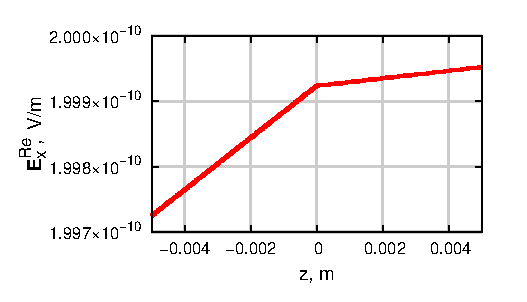
\includegraphics[scale=1]{research-2/650/ExR.eps}
	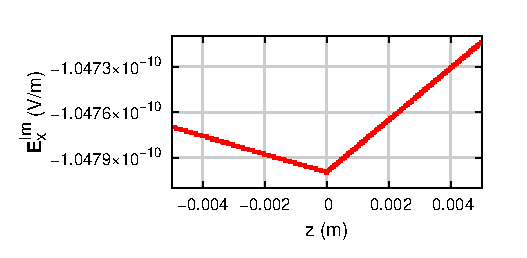
\includegraphics[scale=1]{research-2/650/ExI.eps}
	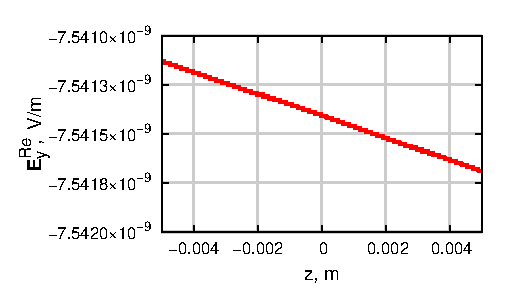
\includegraphics[scale=1]{research-2/650/EyR.eps}
	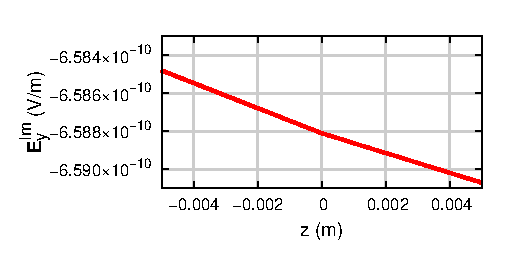
\includegraphics[scale=1]{research-2/650/EyI.eps}
	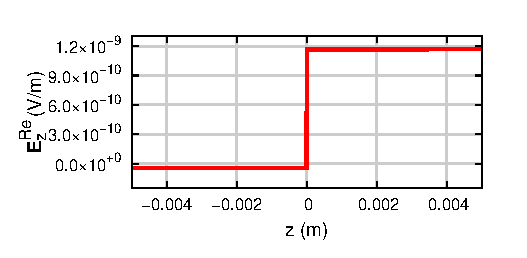
\includegraphics[scale=1]{research-2/650/EzR.eps}
	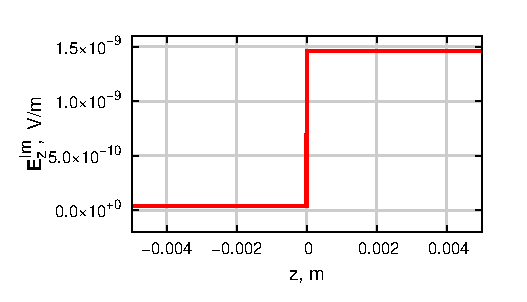
\includegraphics[scale=1]{research-2/650/EzI.eps}
	\caption{графики компонент электрического поля на контактных границах}
	\label{fig:res2:650_3}
\end{figure}

Как видно из графиков на рисунке \ref{fig:res2:650_3}, разрывна только нормальная компонента $\mathbf{E}_z$, следовательно, условия (\ref{eq:maxwell:tangent_E})-(\ref{eq:maxwell:normal_D}) выполнены.

\subsubsection{Графическое представление результатов}
На рисунках \ref{fig:res2:field_sca}, \ref{fig:res2:field_vec} и \ref{fig:res2:field_y0} показаны картины электрического поля, полученные при параметрах $h=5$~м, $\chi_{\Omega_1} = (4, 0)$, $\chi_{\Omega_2} = (1, 6)$, $\chi_{\Omega_2} = (3, 2)$, $m=3$, $l_k = 600$~м и $\delta_k = 100$~м. На рисунках \ref{fig:res2:field_sca_a}, \ref{fig:res2:field_vec_a} и \ref{fig:res2:field_y0_a} представлено решение с PML-слоем; \ref{fig:res2:field_sca_b}, \ref{fig:res2:field_vec_b} и \ref{fig:res2:field_y0_b} -- решение с <<большим баком>>.

\begin{spacing}{1.0}
\setlength{\parskip}{0pt}

\begin{figure}[H]
	\centering
	\subfloat[][]{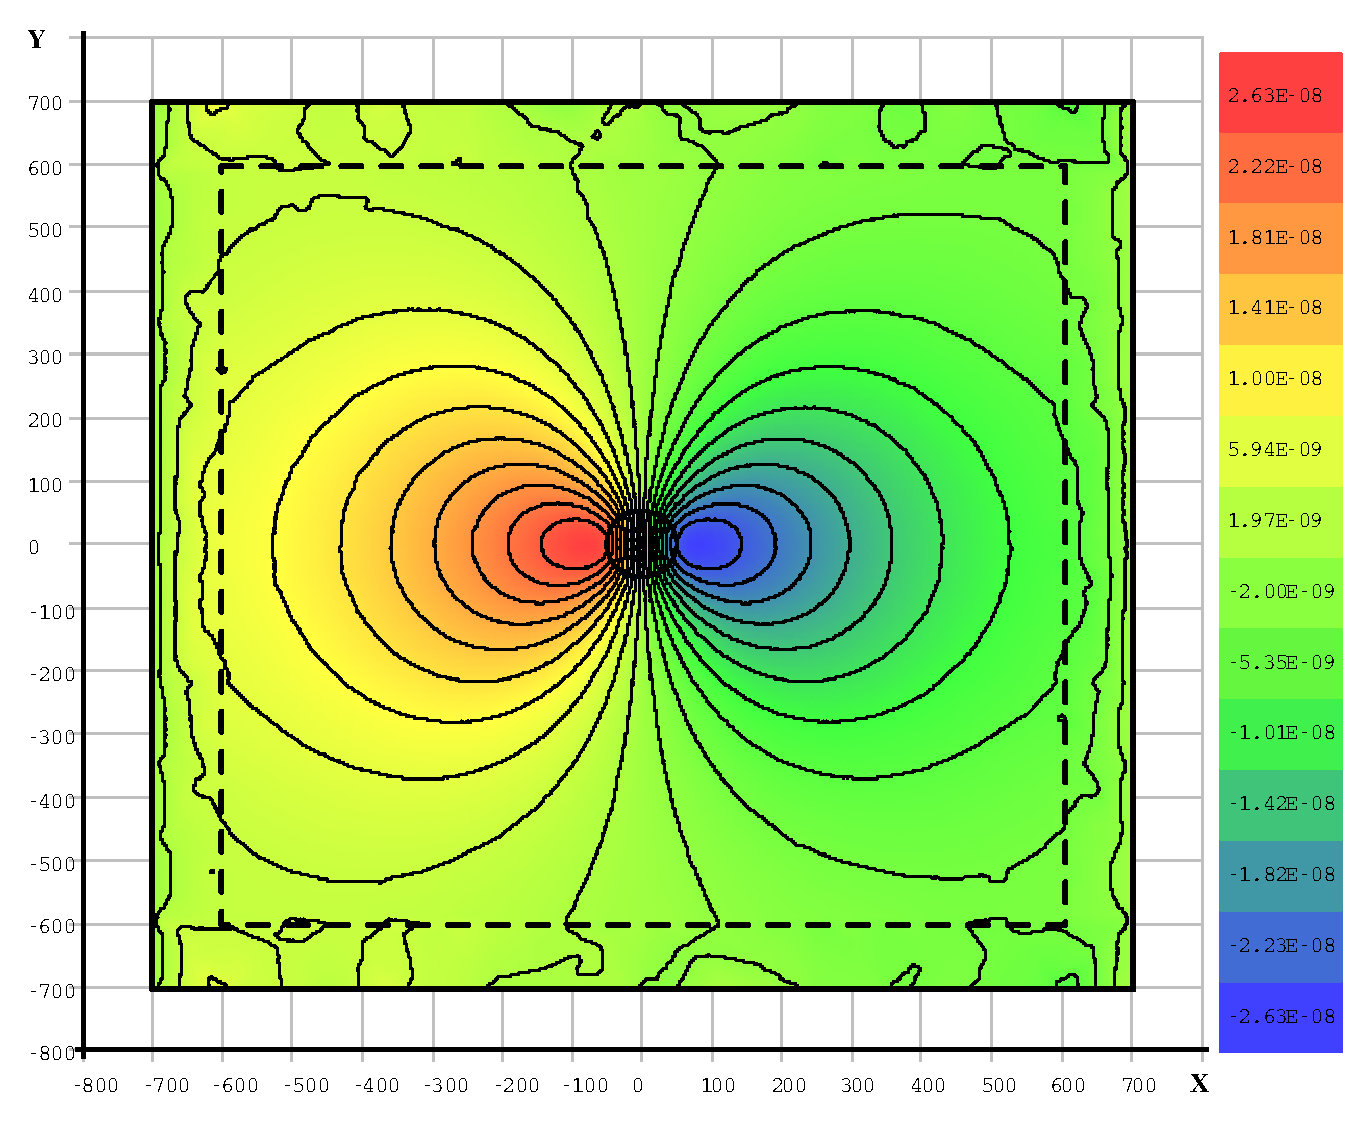
\includegraphics[scale=0.35]{research-2/field/airloop/pml/airloop_pml_z=-10_EyR.eps}\label{fig:res2:field_sca_a}}
	~~
	\subfloat[][]{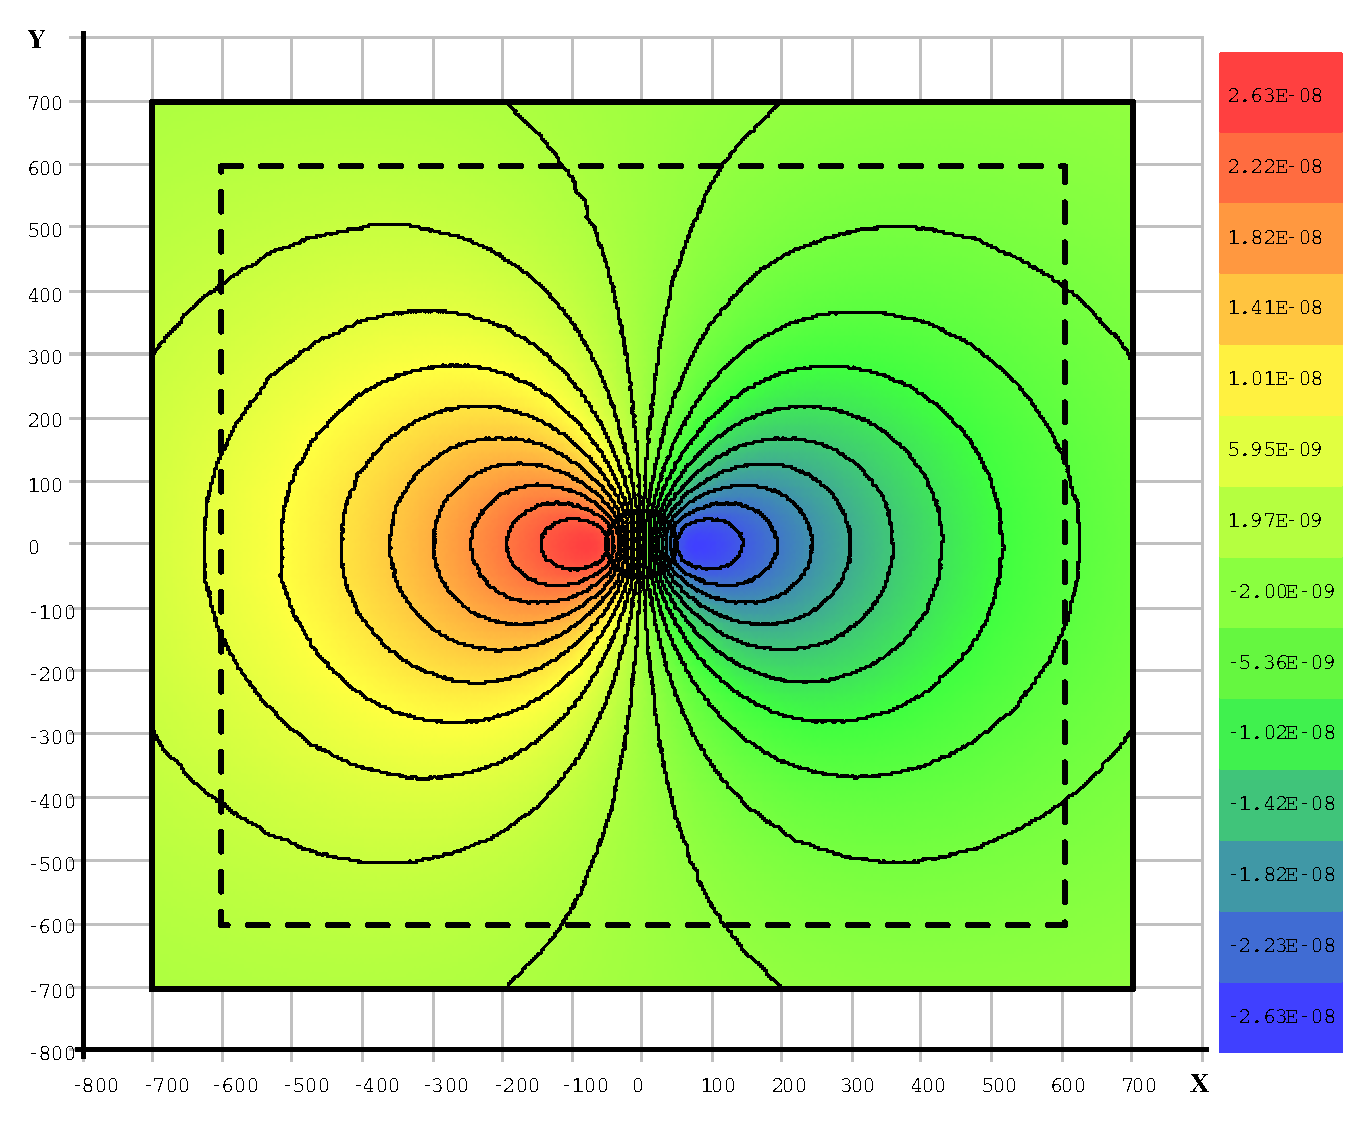
\includegraphics[scale=0.35]{research-2/field/airloop/std/airloop_std_z=-10_EyR.eps}\label{fig:res2:field_sca_b}}
	\caption{$\Re(\mathbf{E}_y)$ в сечении плоскостью $z=-10$~м}
	\label{fig:res2:field_sca}
\end{figure}

\vspace{-0.8cm}

\begin{figure}[H]
	\centering
	\subfloat[][]{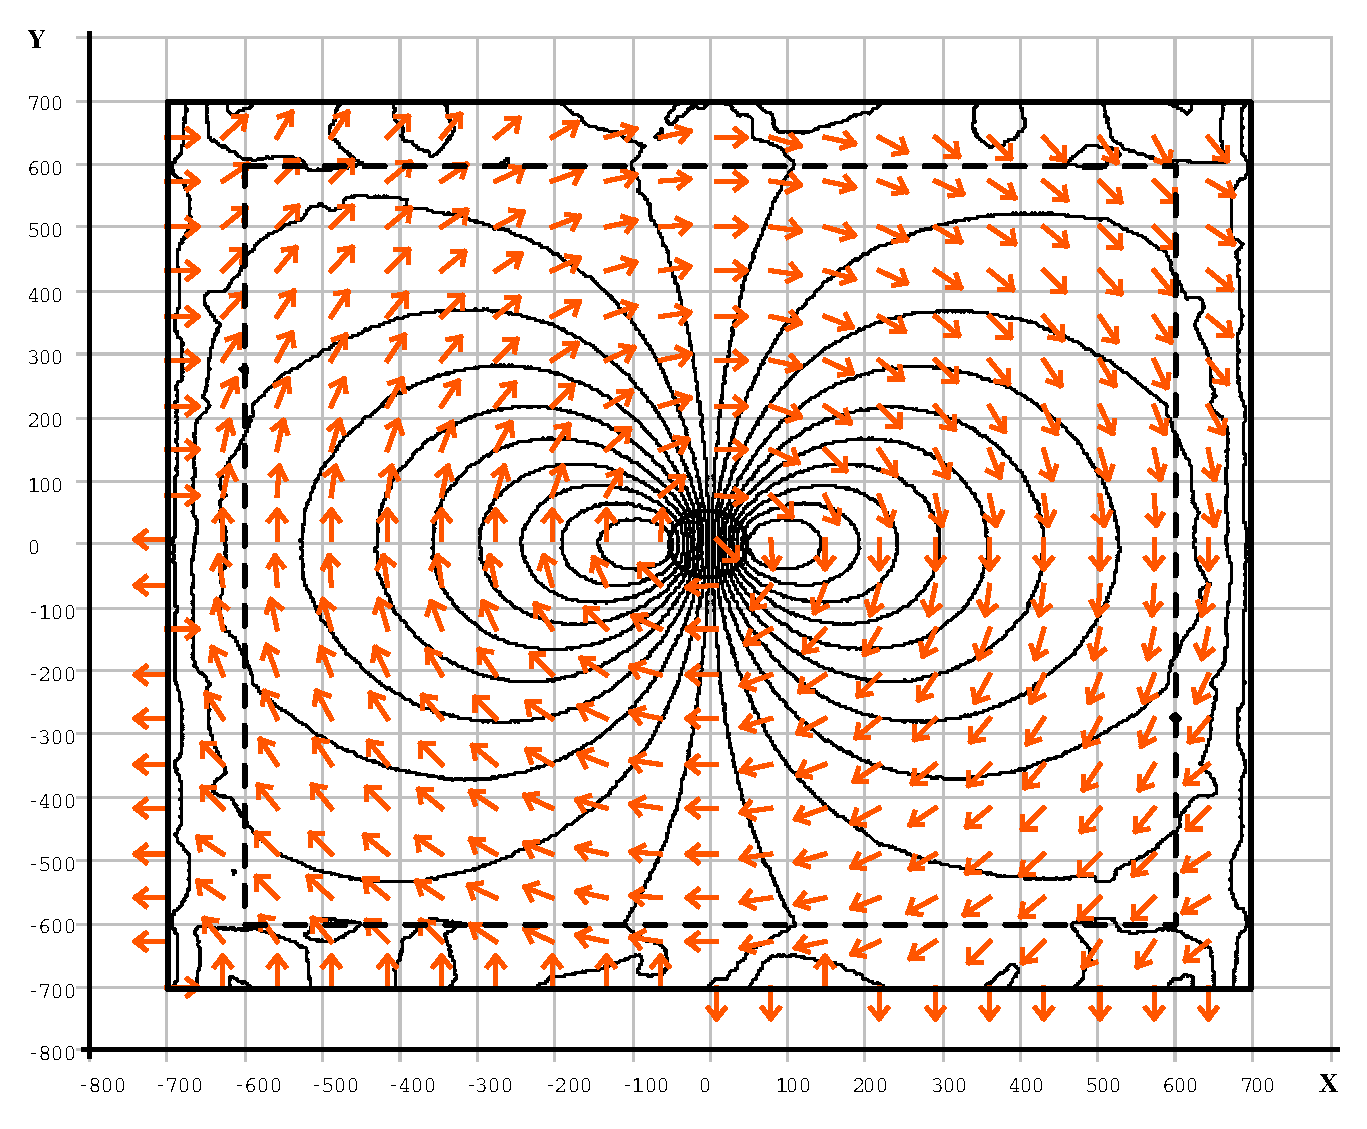
\includegraphics[scale=0.35]{research-2/field/airloop/pml/airloop_pml_z=-10_EyR_vec.eps}\label{fig:res2:field_vec_a}}
	~~
	\subfloat[][]{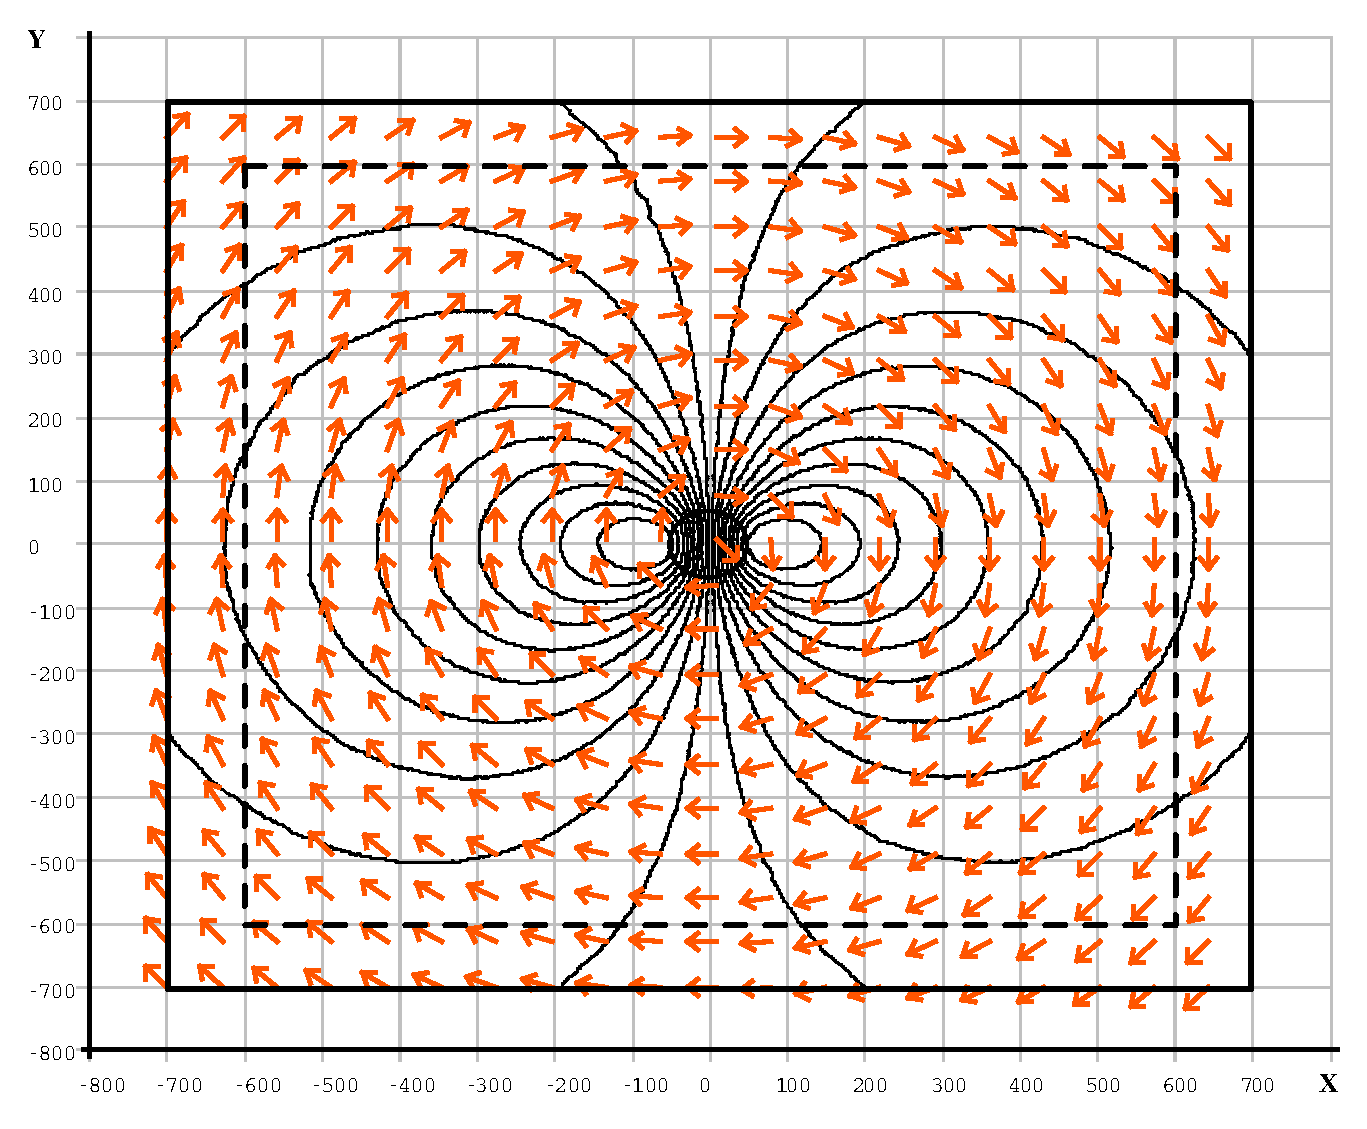
\includegraphics[scale=0.35]{research-2/field/airloop/std/airloop_std_z=-10_EyR_vec.eps}\label{fig:res2:field_vec_b}}
	\caption{изолинии $\Re(\mathbf{E}_y)$ и векторы $\left( \Re(\mathbf{E}_x) , \Re(\mathbf{E}_y) \right)^T$ в сечении плоскостью $z=-10$~м}
	\label{fig:res2:field_vec}
\end{figure}

\vspace{-0.8cm}

\begin{figure}[H]
	\centering
	\subfloat[][]{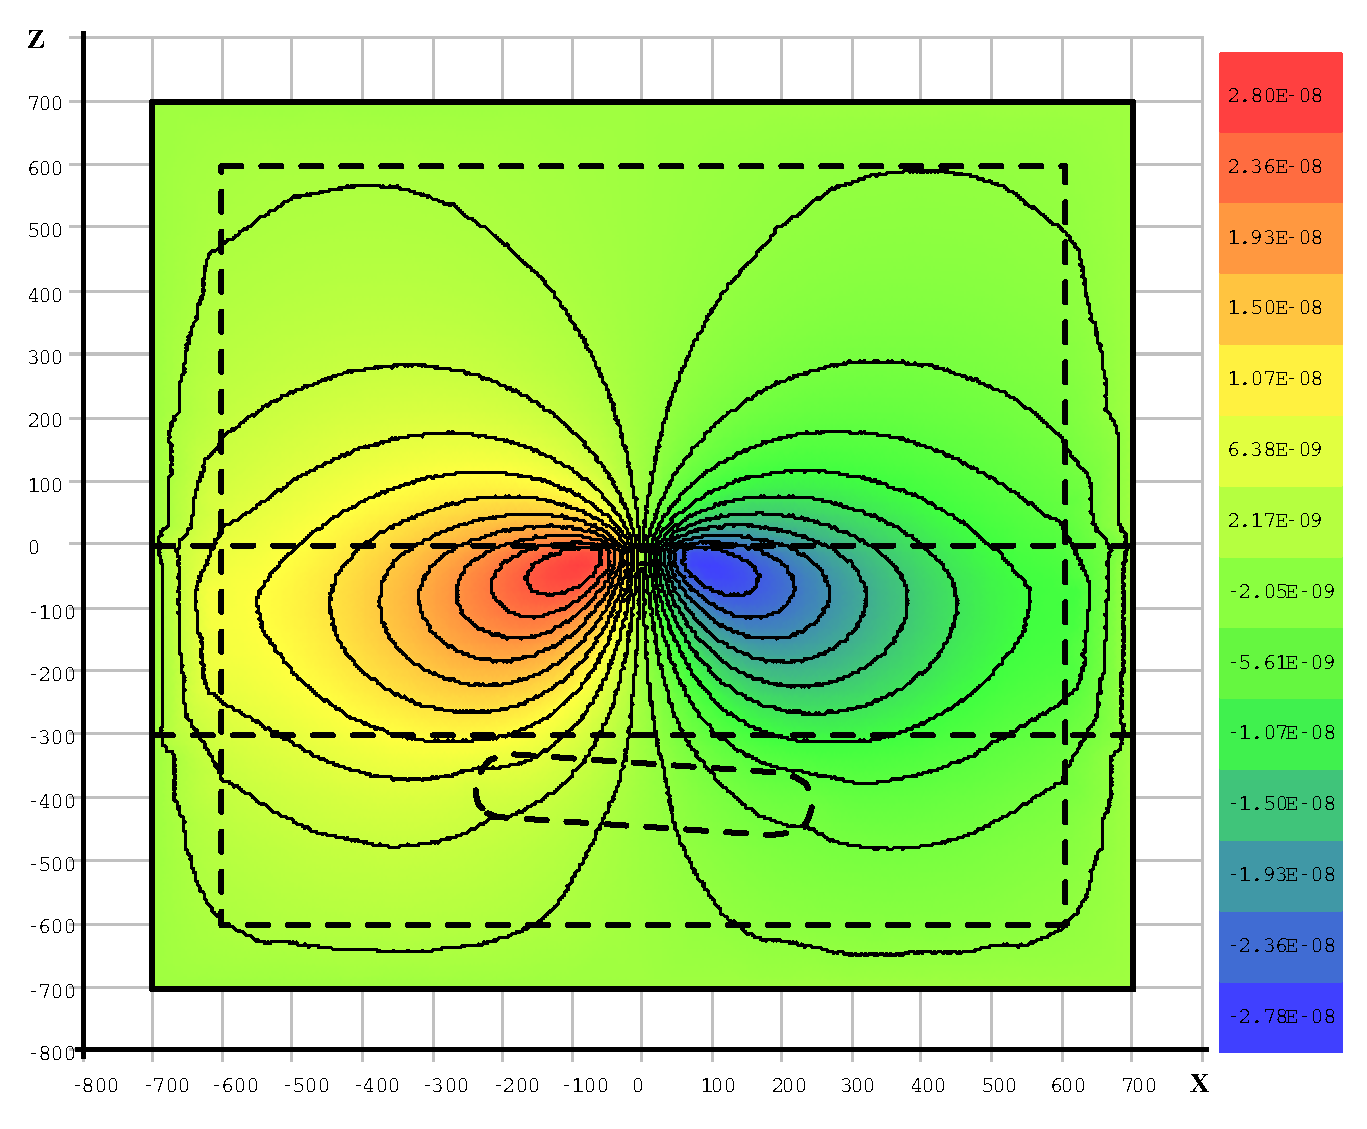
\includegraphics[scale=0.35]{research-2/field/airloop/pml/airloop_pml_y=0_EyR.eps}\label{fig:res2:field_y0_a}}
	~~
	\subfloat[][]{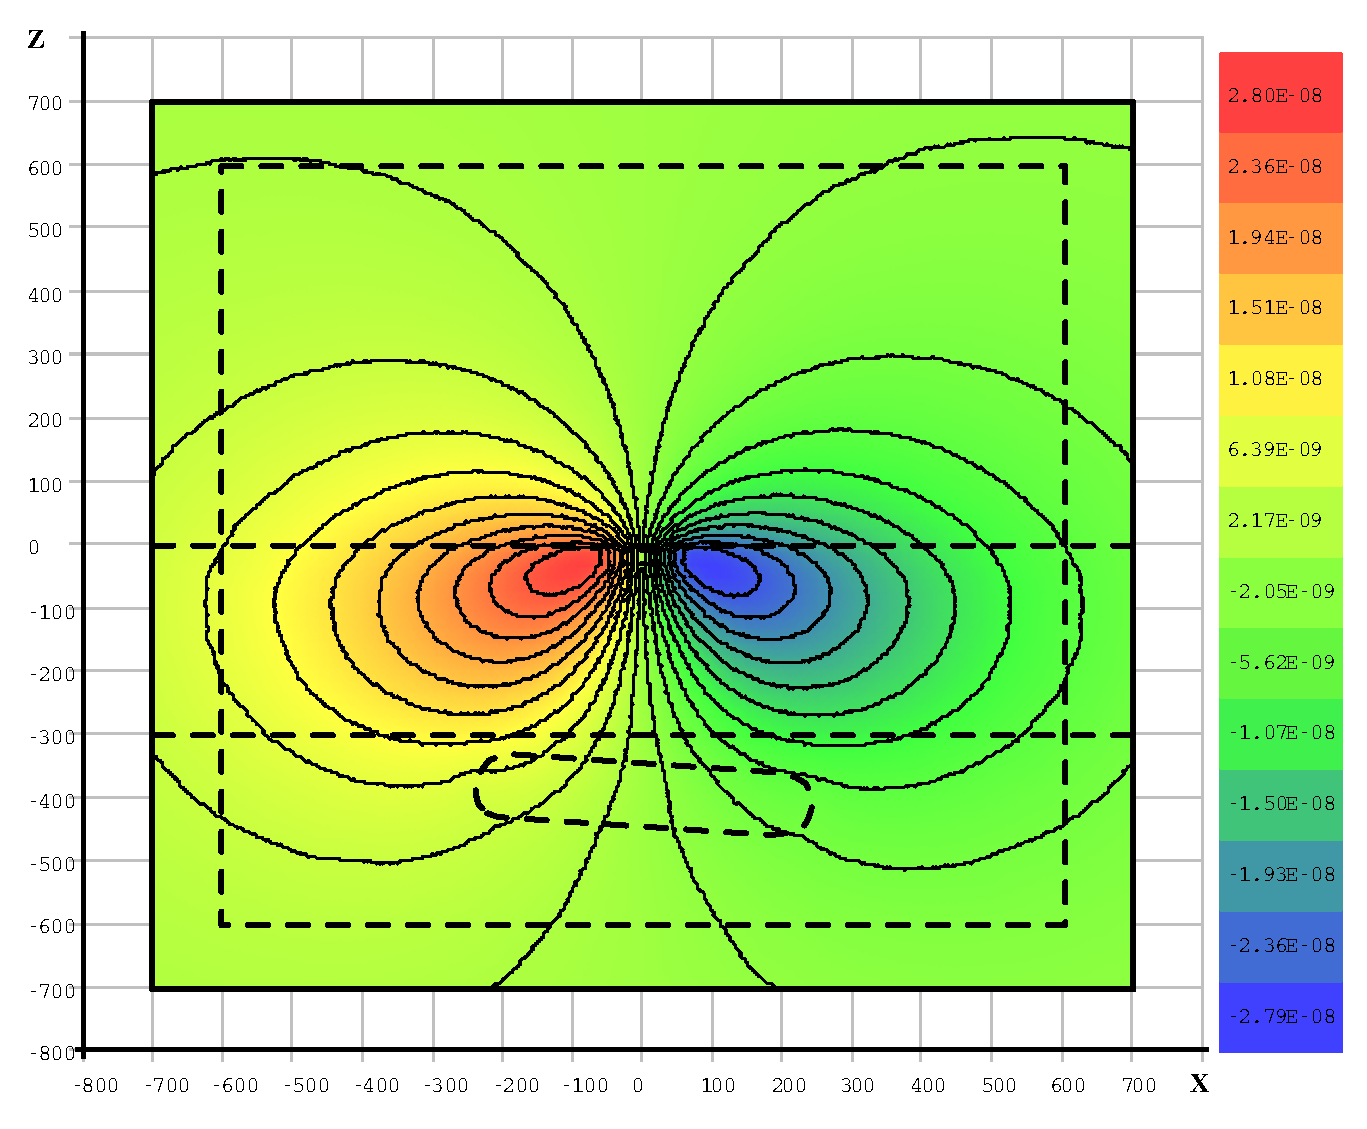
\includegraphics[scale=0.35]{research-2/field/airloop/std/airloop_std_y=0_EyR.eps}\label{fig:res2:field_y0_b}}
	\caption{$\Re(\mathbf{E}_y)$ в сечении плоскостью $y=0$}
	\label{fig:res2:field_y0}
\end{figure}

\end{spacing}

% =============================================================================

\subsubsection{Анализ целесообразности применения PML-слоя}
Наибольшее влияние на точность получаемого решения при введении PML-слоя оказывают коэффициент комплексного растяжения координат $\chi$ и $l$ -- размер области, на границе которой вводится PML-слой. При увеличении размера внутренней области ожидаемо увеличивается размер СЛАУ, поэтому этот параметр при решении реальных задач следует не варьировать, а выбрать как некоторое ограничение. Таким образом, в первую очередь стоит проводить поиск оптимального значения именно для коэффициента растяжения $\chi$. Выбор толщины PML-слоя влияет на точность решения незначительно, поэтому достаточно лишь убедиться, что она выбрана в подходящих для задачи пределах -- не слишком большой и не слишком маленькой.

В рассмотренном виде применение PML-слоя для сокращения области моделирования задач низкочастотной морской геоэлектрики незначительно уменьшает размерность СЛАУ и, в большинстве случаев, не приводит к существенному сокращению времени решения задачи. Одной из причин этого может быть то, что основное растяжение приходится на вещественные компоненты координат. Это приводит к значительной <<вытянутости>> тетраэдров внутри PML-слоя и, как следствие, сильному ухудшению свойств матрицы СЛАУ и увеличению времени решения. Параллелепипедальные конечные элементы лишены подобного недостатка, поэтому для них можно проводить комплексное растяжение в гораздо больших диапазонах. Однако, такие элементы не подходят для аппроксимации сколь-либо сложных областей. Для использования в одной сетке и тетраэдральных, и параллелепипедальных конечных элементов можно применять специальные переходные элементы {\color{red}\textbf{[ССЫЛКИ!]}}, либо воспользоваться неконформными методами {\color{red}\textbf{[ССЫЛКИ!]}}. %TODO ССЫЛКИ

% =============================================================================

\subsection{Задача, приближенная к реальной}
В этом исследовании рассмотрим поведение электрического поля при различном расположении источника этого поля относительно объекта, скрытого в грунте. Различное положение источника обеспечивается за счет <<протаскивания>> его на некотором расстоянии от морского дна.

В этом исследовании будем пользоваться базисными функциями второго полного порядка.

\subsubsection{Описание расчетной области}
Схематичное изображение расчетной области показано на рисунке \ref{fig:res3:area}, где $\Omega_1$ -- воздух ($\sigma=10^{-6}$ См/м, $\mu=\mu_0$, $\varepsilon=\varepsilon_0$); $\Omega_2$ -- морская вода ($\sigma=3.3$ См/м, $\mu=\mu_0$, $\varepsilon=\varepsilon_0$); $\Omega_3$ -- грунт ($\sigma=0.2$ См/м, $\mu=\mu_0$, $\varepsilon=\varepsilon_0$); $\Omega_4$ -- углеводороды ($\sigma=10^{-2}$~См/м, $\mu=\mu_0$, $\varepsilon=\varepsilon_0$); $L_1$, $L_2$ и $L_3$ -- размеры области моделирования по осям $x$, $y$ и $z$ соответственно; $L_1 = L_2 = L_3 = 6000$~м; $h_1=600$~м -- толщина $\Omega_2$; $l_1=400$~м, $h_3=75$~м, $h_2=120$~м -- длина, толщина и глубина объекта $\Omega_4$ соответственно.
\begin{figure}[H]
	\centering
	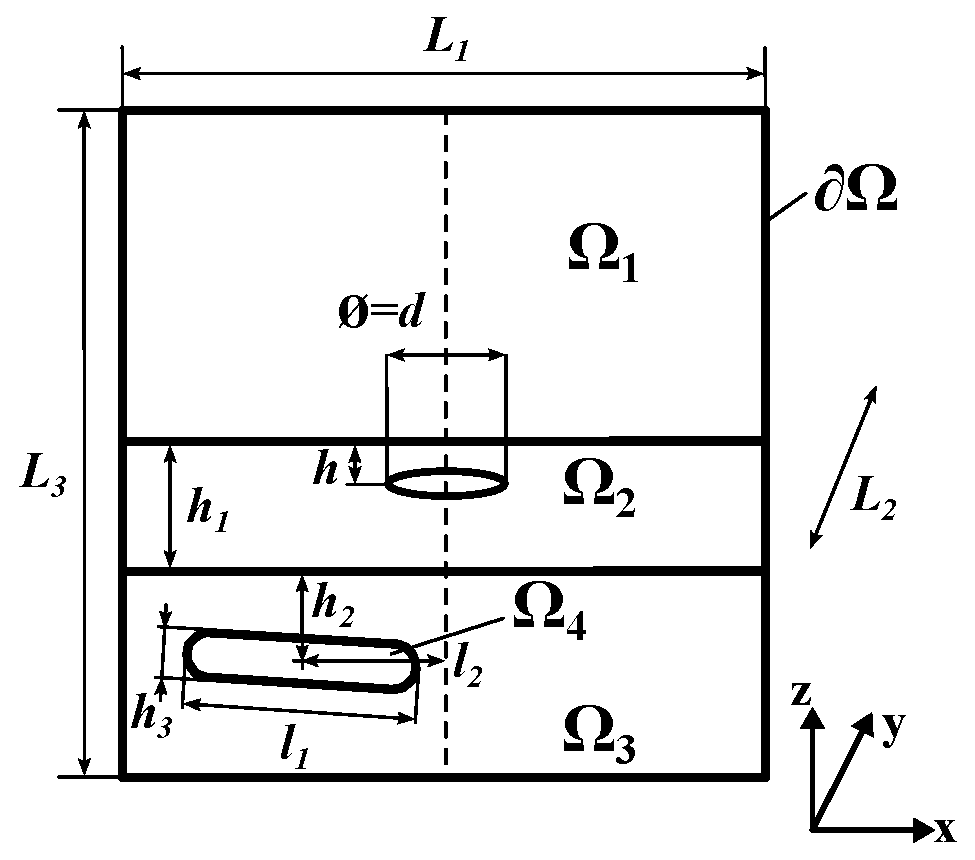
\includegraphics[scale=0.7]{research-3/area/area_3layers_shift_3.eps}
	\caption{схематичное изображение расчетной области}
	\label{fig:res3:area}
\end{figure}

Источником электрического поля является петля диаметром $d=100$ м с током частотой 1 Гц, расположенная в воде на расстоянии $h=590$ м от границы раздела сред воздух-вода (в 10 метрах над поверхностью грунта). Объект $\Omega_4$, как и в предыдущих исследованиях, представляет собой скругленный прямоугольный параллелепипед с двумя равными сторонами, наклоненный под углом $5^{\circ}$.

В этой области рассмотрим электрическое поле при различных смещениях объекта относительно источника ($l_2=-300$, $-200$, $-100$ и $0$ м), а также сравним с электрическим полем в случае проводящего объекта ($\sigma=10^2$ См/м).

\subsubsection{Конечноэлементная сетка}
Фрагмент $x \in [-600,0]$, $y \in [-600,600]$ $z \in [-1000,600]$ одной из конечноэлементных сеток, использованных для проведения исследования, представлен на рисунке \ref{fig:res3:mesh}.

\begin{figure}[H]
	\centering
	% trim=left bottom right top
	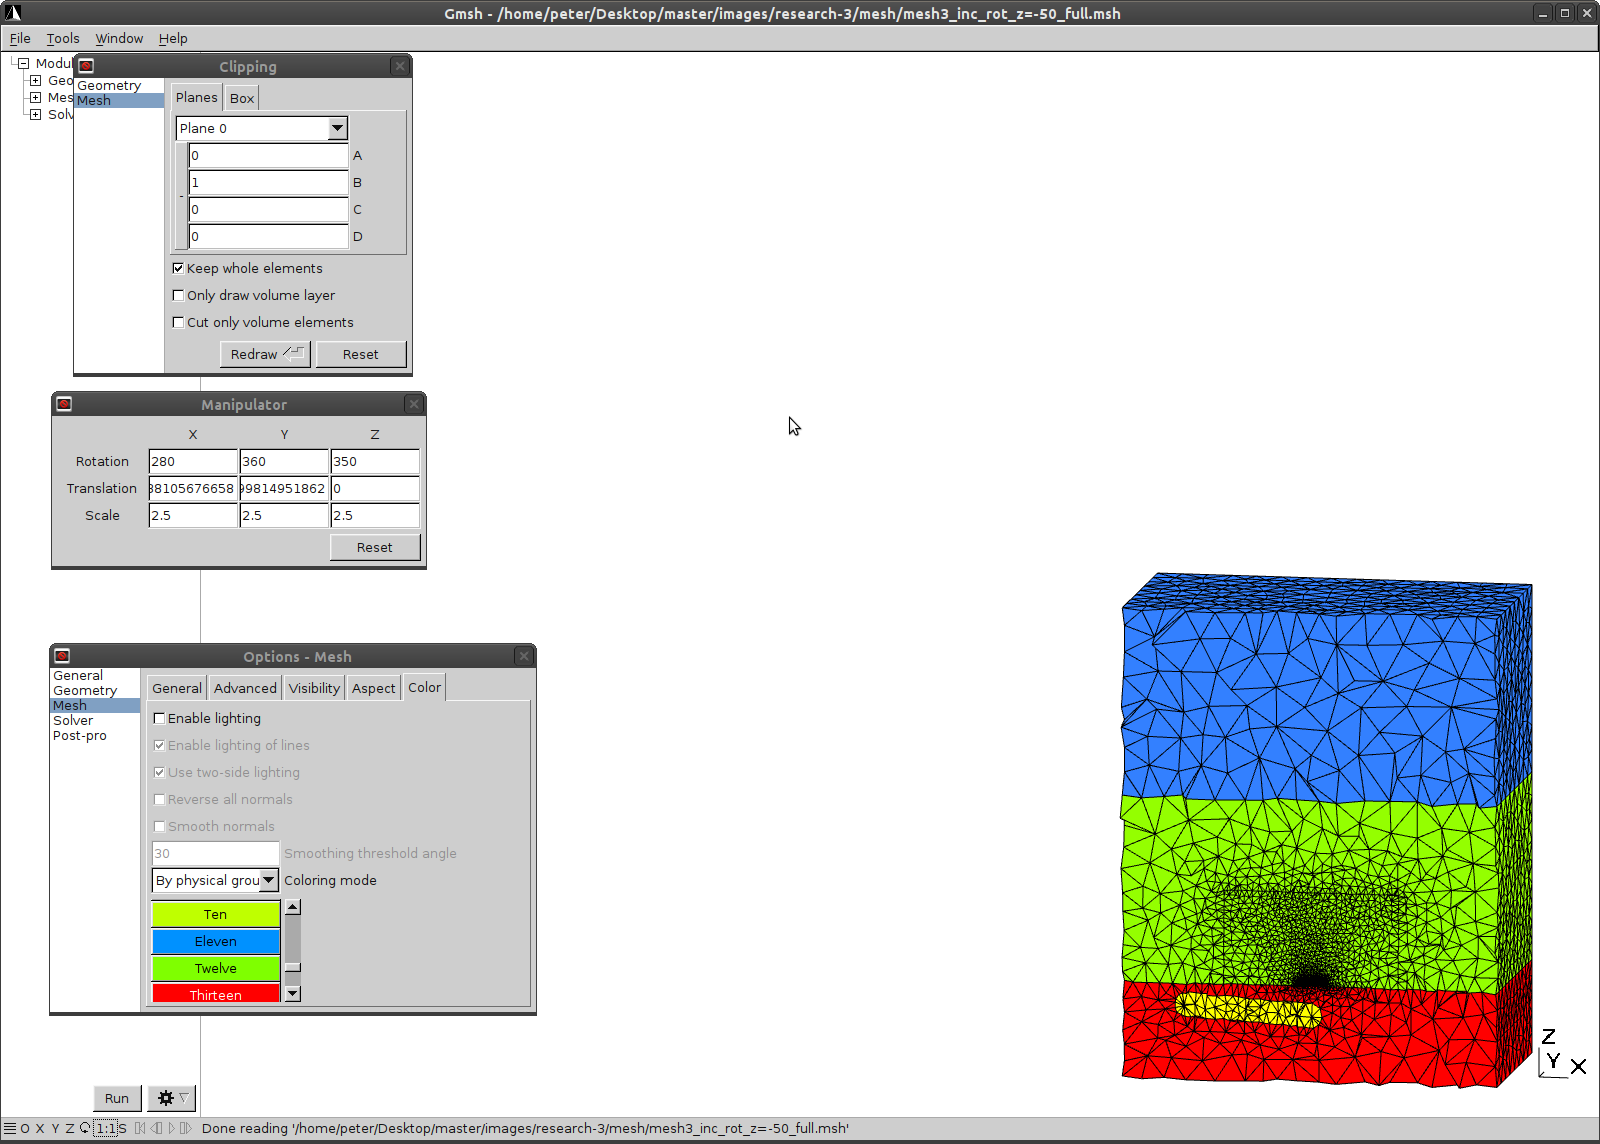
\includegraphics[trim=390mm 20mm 5mm 195mm,clip,scale=0.5]{research-3/mesh/mesh.png}
	\caption{фрагмент конечноэлементной сетки}
	\label{fig:res3:mesh}
\end{figure}

\subsubsection{Результаты вычислительного эксперимента}
На рисунках \ref{fig:res3:0_EyR}-\ref{fig:res3:300_EzR} показано графическое представление напряженности электрического поля $\mathbf{E}$, на рисунках под буквой <<а>>~(слева) -- для объекта с $\sigma=10^{-2}$~См/м, под буквой <<б>>~(справа) -- для объекта с $\sigma=10^{2}$~См/м.

\begin{spacing}{1.0}
\setlength{\parskip}{0pt}

\begin{figure}[H]
	\centering
	\subfloat[][]{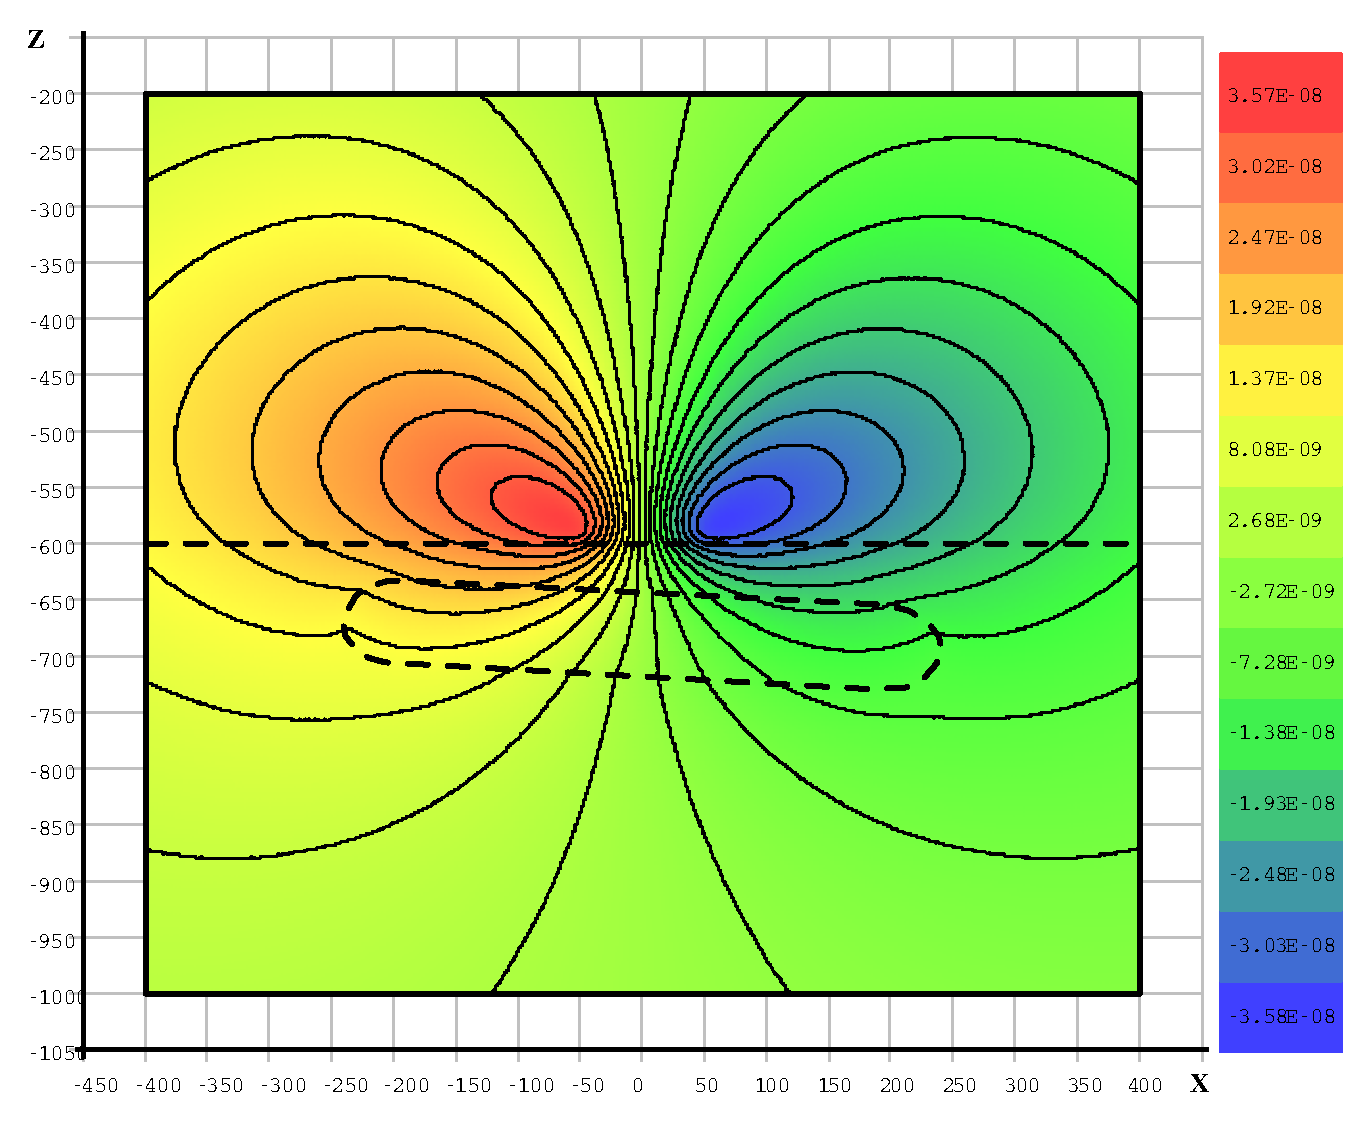
\includegraphics[scale=0.35]{research-3/fields/images/0/0_no_y=0_EyR.eps}\label{fig:res3:0_EyR_a}}
	\text{~~}
	\subfloat[][]{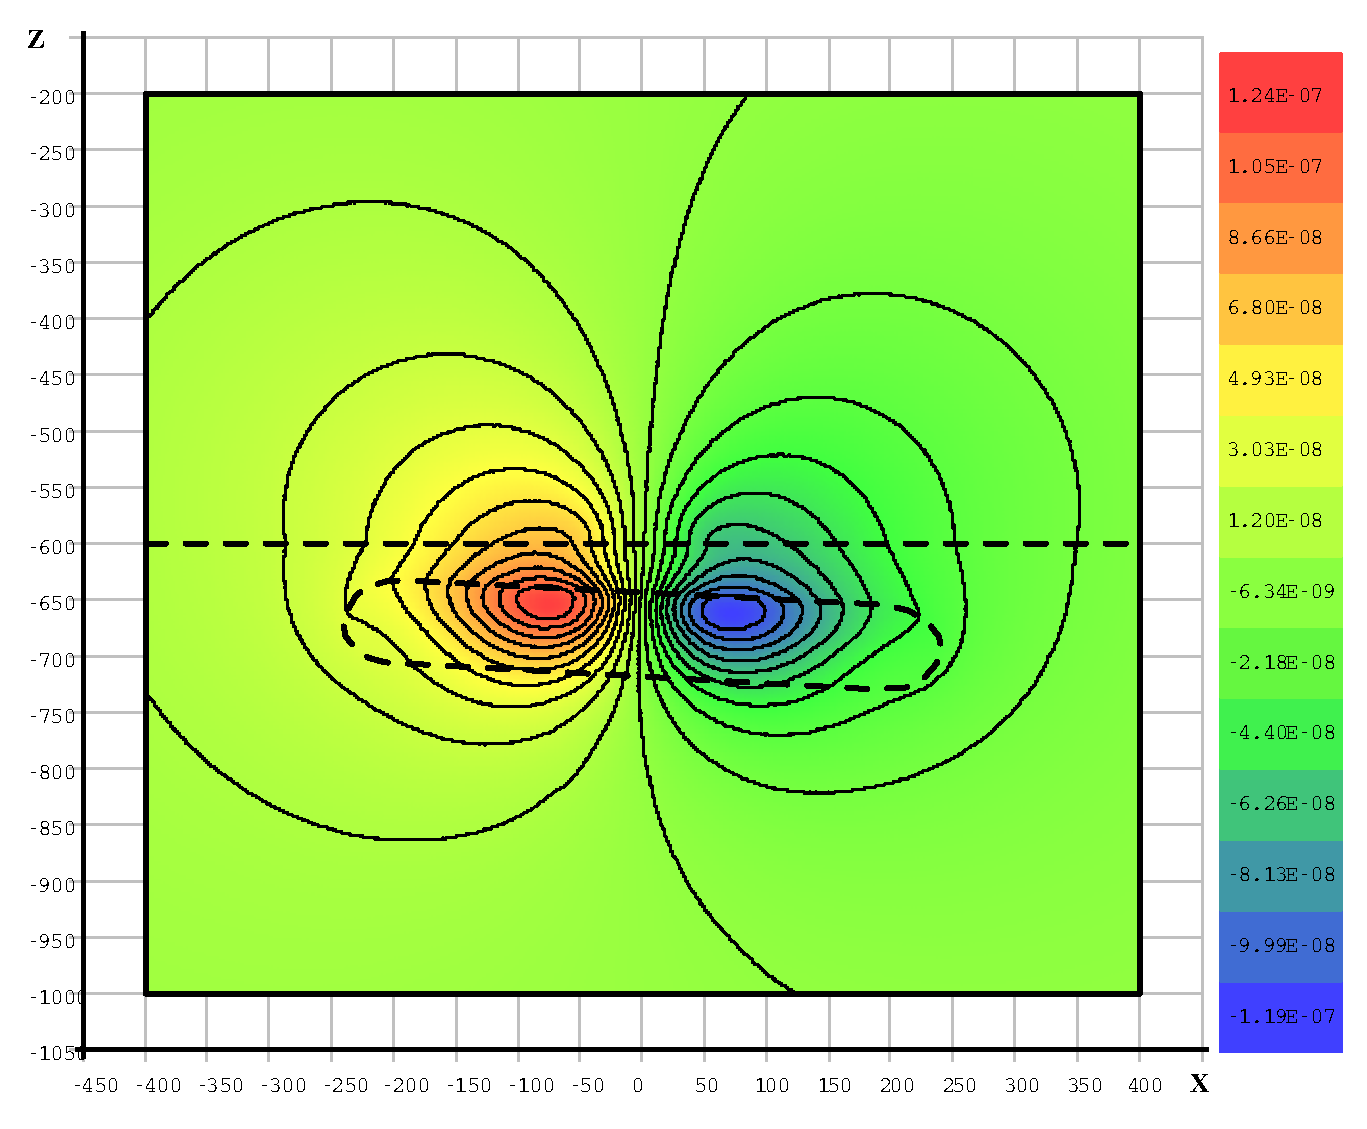
\includegraphics[scale=0.35]{research-3/fields/images/0/0_yes_y=0_EyR.eps}\label{fig:res3:0_EyR_b}}
	\caption{$\Re(\mathbf{E}_y)$ при $l_2=0$ в сечении $y=0$}
	\label{fig:res3:0_EyR}
\end{figure}

\vspace{-0.8cm}

\begin{figure}[H]
	\centering
	\subfloat[][]{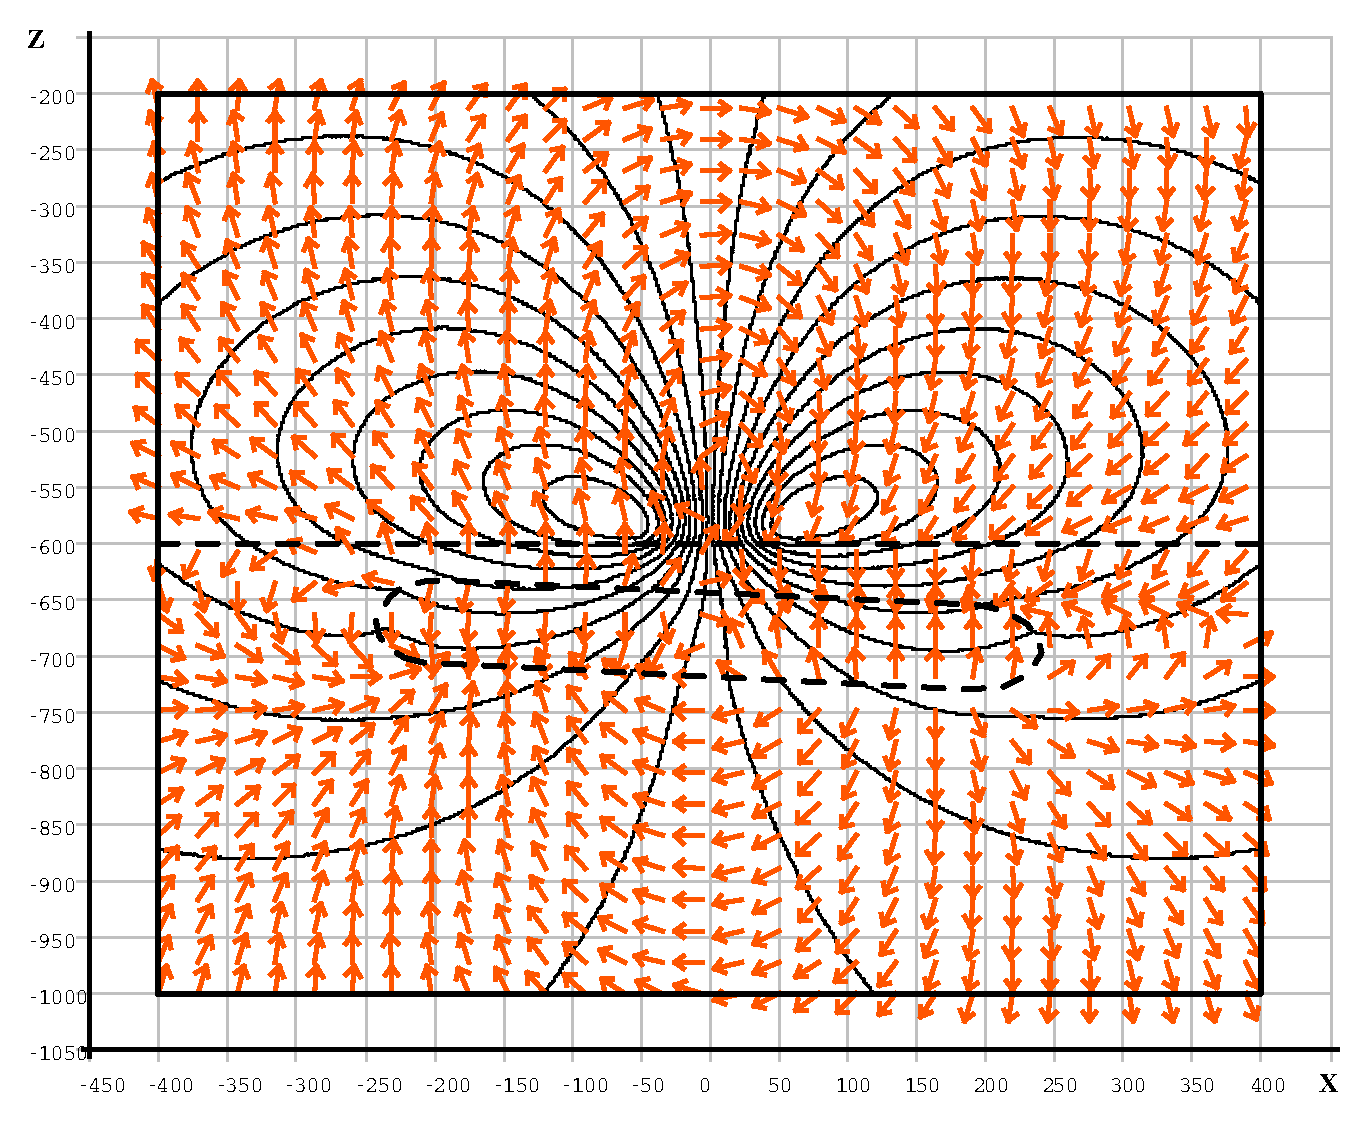
\includegraphics[scale=0.35]{research-3/fields/images/0/0_no_y=0_vec.eps}\label{fig:res3:0_vec_a}}
	\text{~~}
	\subfloat[][]{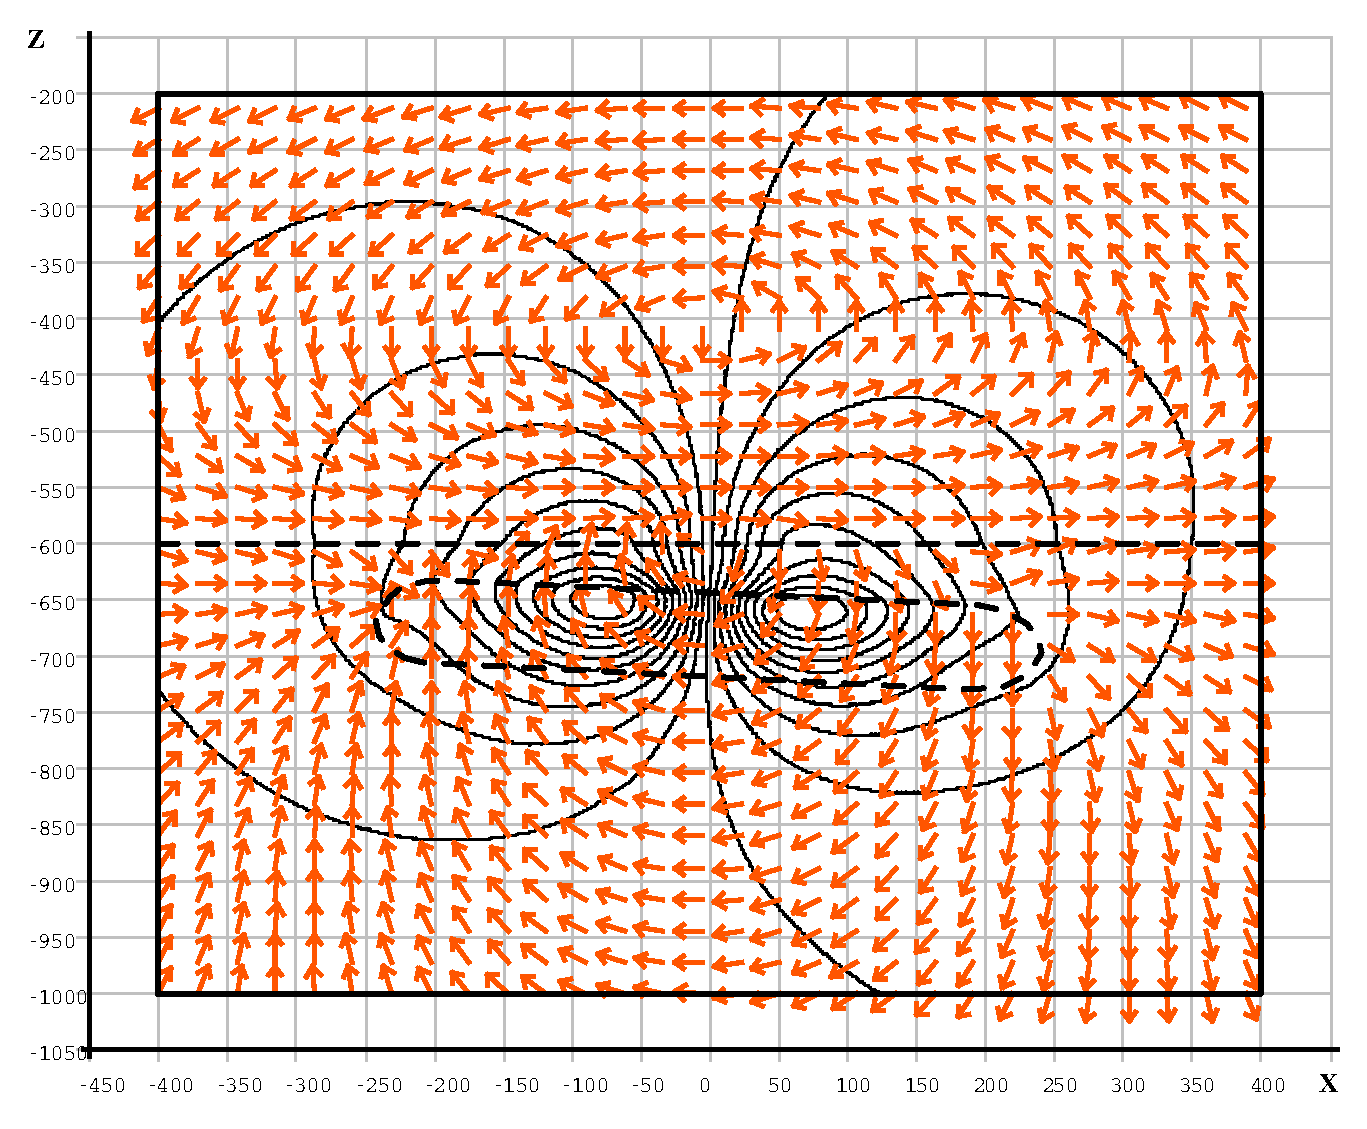
\includegraphics[scale=0.35]{research-3/fields/images/0/0_yes_y=0_vec.eps}\label{fig:res3:0_vec_b}}
	\caption{векторы $(\Re(\mathbf{E}_x), \Re{\mathbf{E}_z})^T$, изолинии $\Re(\mathbf{E}_y)$ при $l_2=0$ в сечении $y=0$}
	\label{fig:res3:0_vec}
\end{figure}

\vspace{-0.8cm}

\begin{figure}[H]
	\centering
	\subfloat[][]{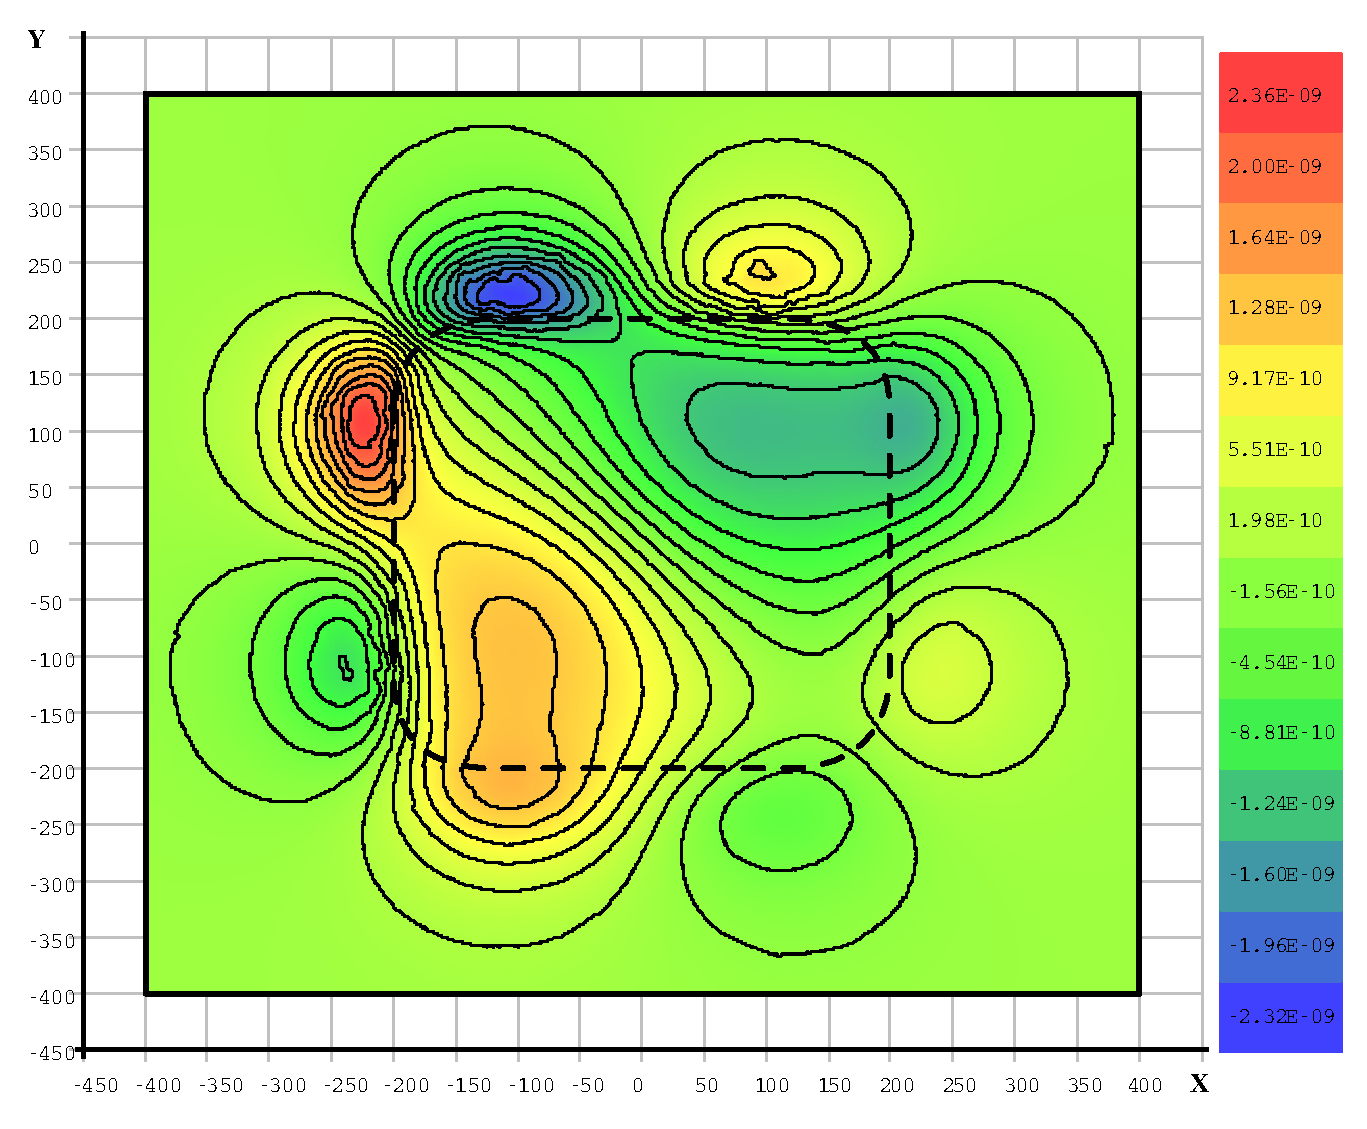
\includegraphics[scale=0.35]{research-3/fields/images/0/0_no_z=-601_EzR.eps}\label{fig:res3:0_EzR_a}}
	\text{~~}
	\subfloat[][]{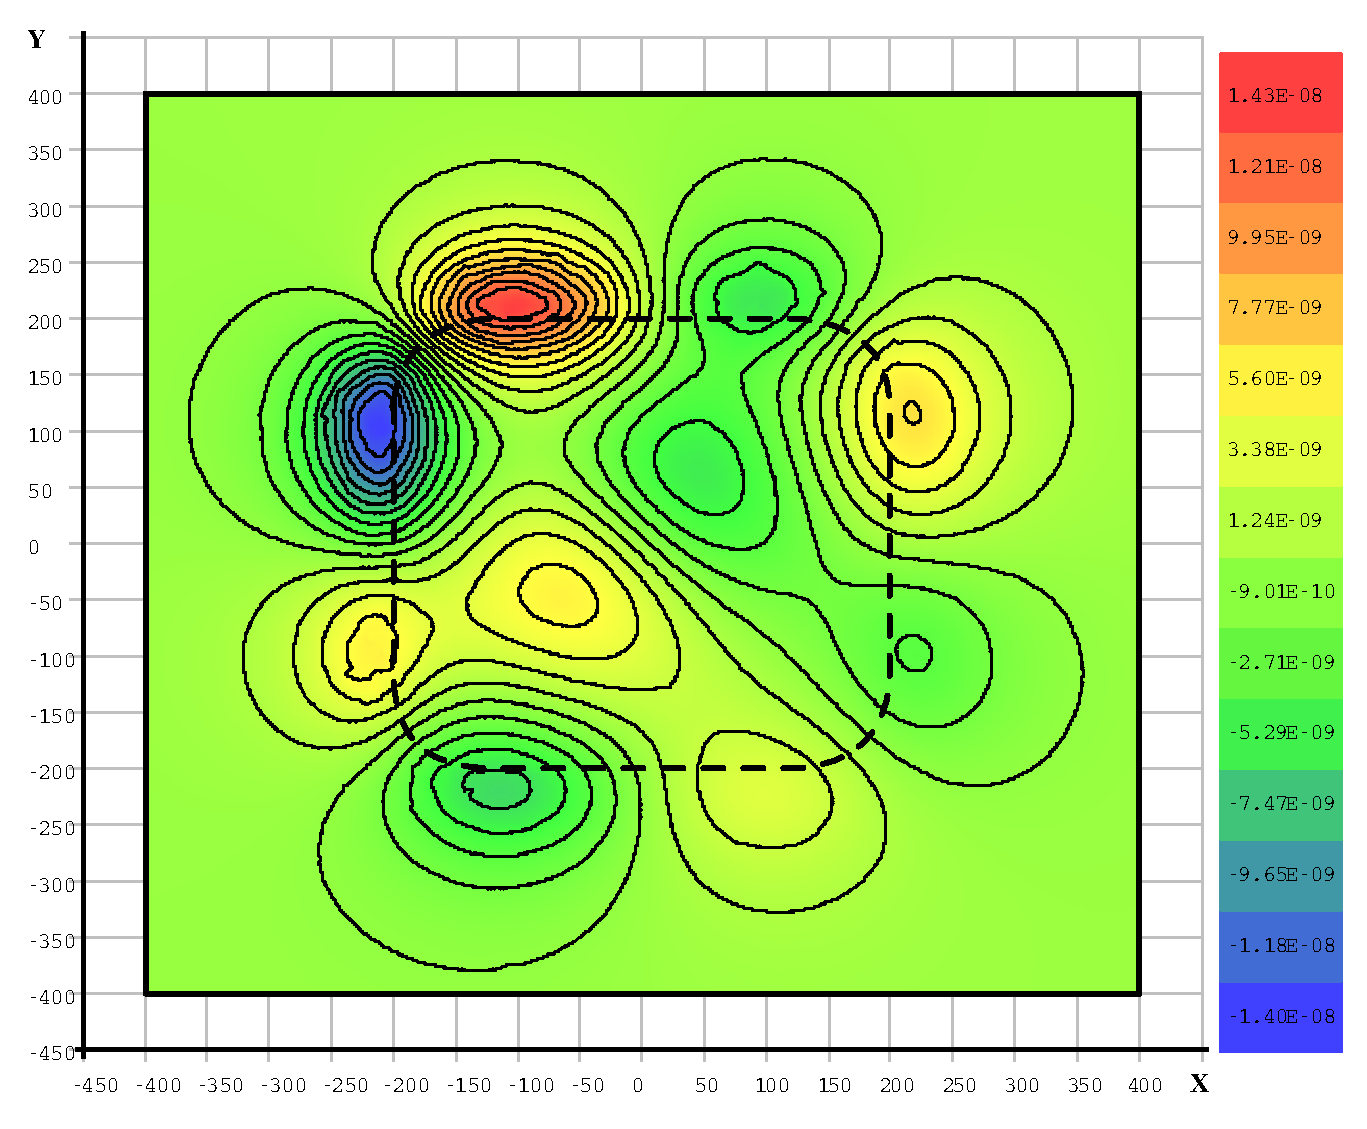
\includegraphics[scale=0.35]{research-3/fields/images/0/0_yes_z=-601_EzR.eps}\label{fig:res3:0_EzR_b}}
	\caption{$\Re(\mathbf{E}_z)$ при $l_2=0$ в сечении $z=-601$}
	\label{fig:res3:0_EzR}
\end{figure}

\vspace{-0.8cm}

\begin{figure}[H]
	\centering
	\subfloat[][]{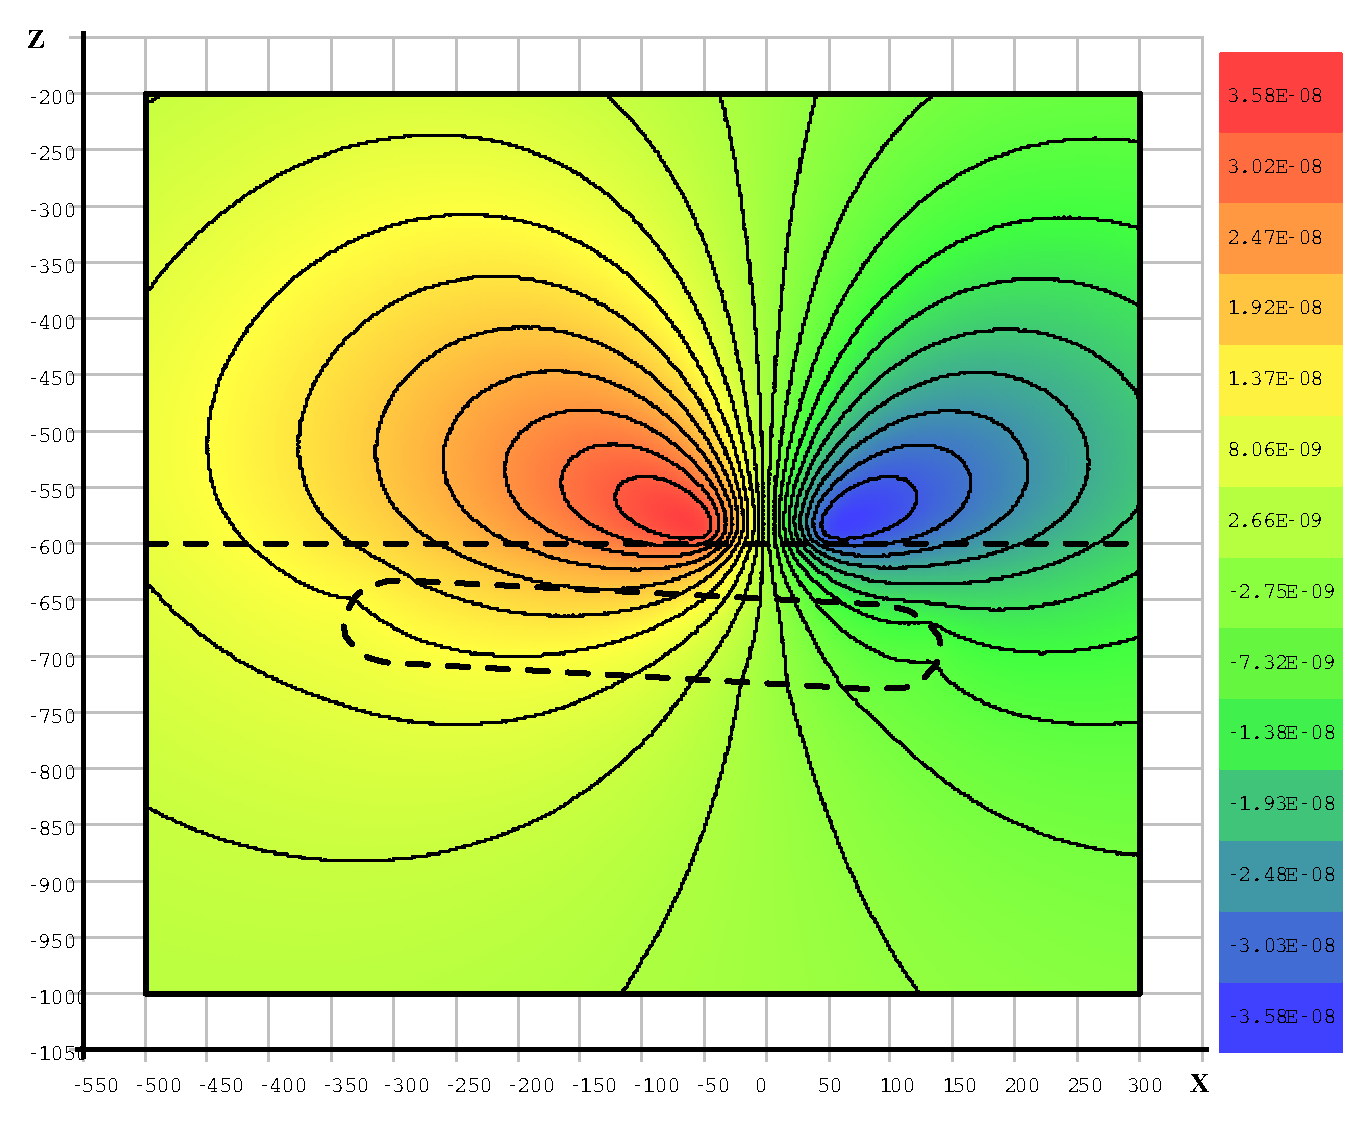
\includegraphics[scale=0.35]{research-3/fields/images/100/100_no_y=0_EyR.eps}\label{fig:res3:100_EyR_a}}
	\text{~~}
	\subfloat[][]{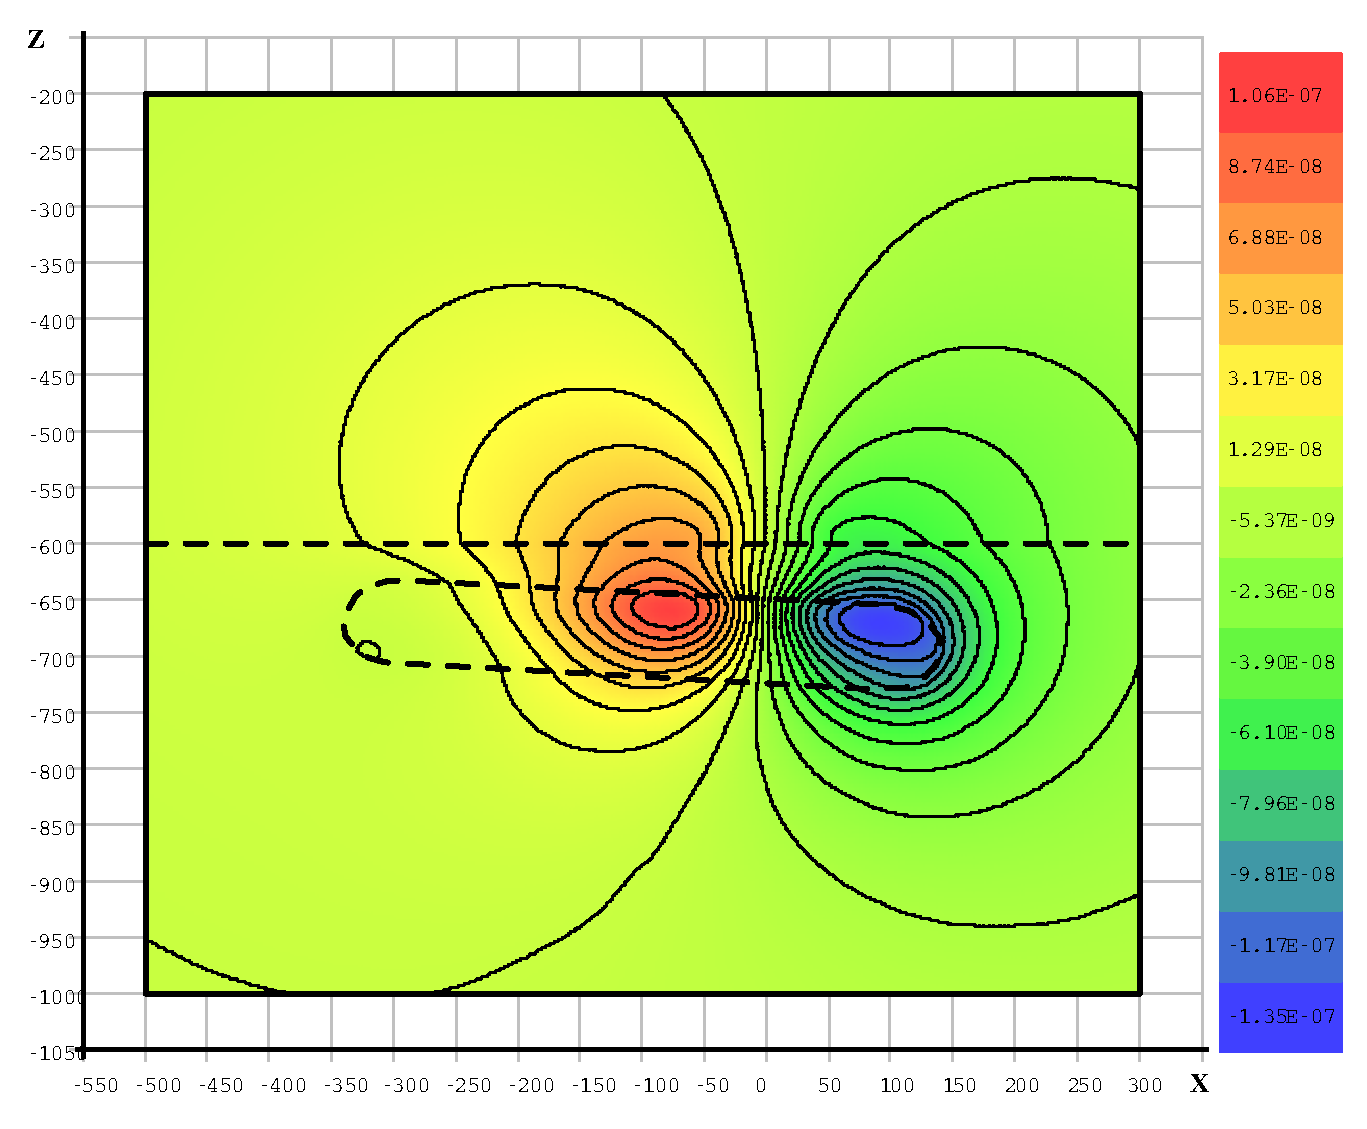
\includegraphics[scale=0.35]{research-3/fields/images/100/100_yes_y=0_EyR.eps}\label{fig:res3:100_EyR_b}}
	\caption{$\Re(\mathbf{E}_y)$ при $l_2=-100$ в сечении $y=0$}
	\label{fig:res3:100_EyR}
\end{figure}

\vspace{-0.8cm}

\begin{figure}[H]
	\centering
	\subfloat[][]{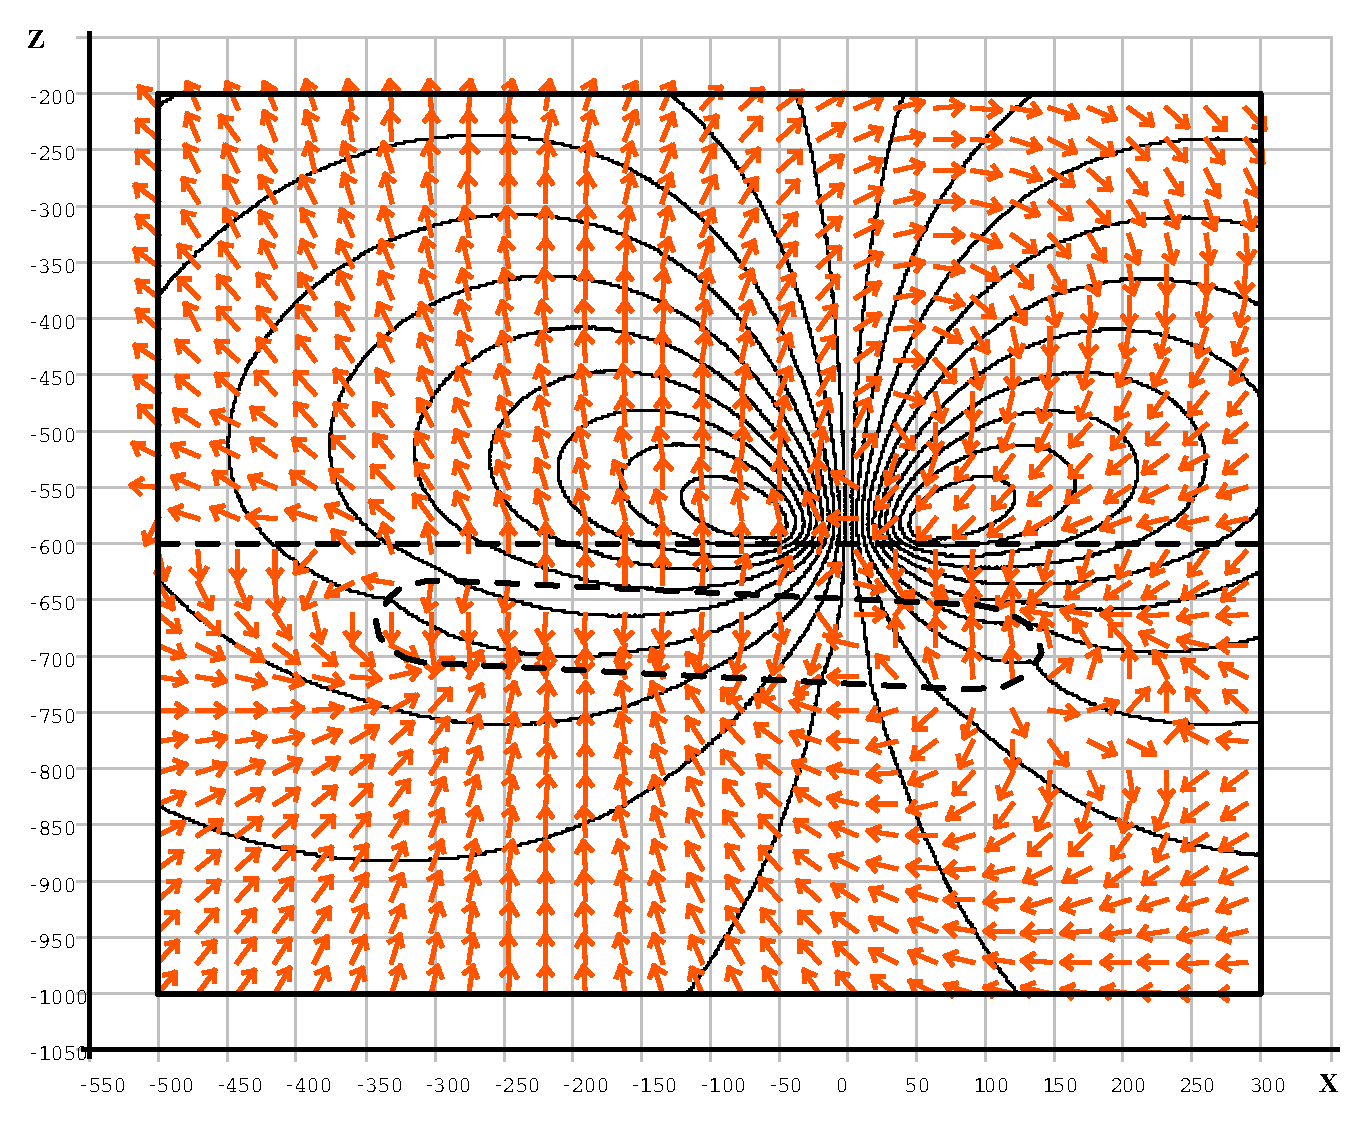
\includegraphics[scale=0.35]{research-3/fields/images/100/100_no_y=0_vec.eps}\label{fig:res3:100_vec_a}}
	\text{~~}
	\subfloat[][]{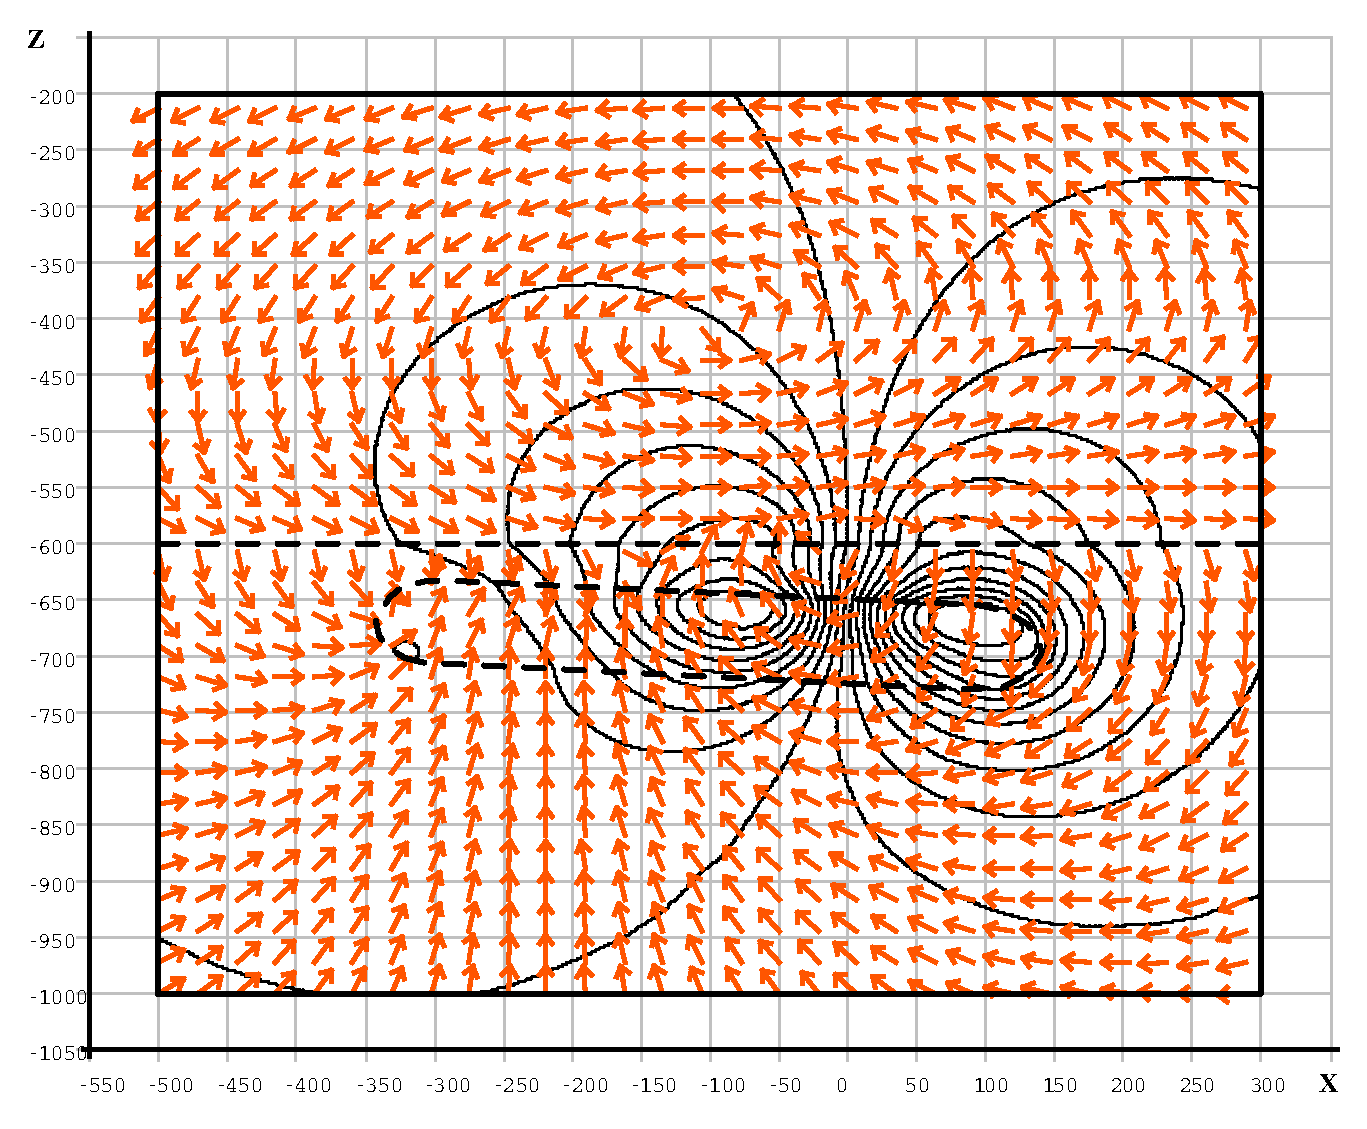
\includegraphics[scale=0.35]{research-3/fields/images/100/100_yes_y=0_vec.eps}\label{fig:res3:100_vec_b}}
	\caption{векторы $(\Re(\mathbf{E}_x), \Re{\mathbf{E}_z})^T$, изолинии $\Re(\mathbf{E}_y)$ при $l_2=-100$ в сечении $y=0$}
	\label{fig:res3:100_vec}
\end{figure}

\vspace{-0.8cm}

\begin{figure}[H]
	\centering
	\subfloat[][]{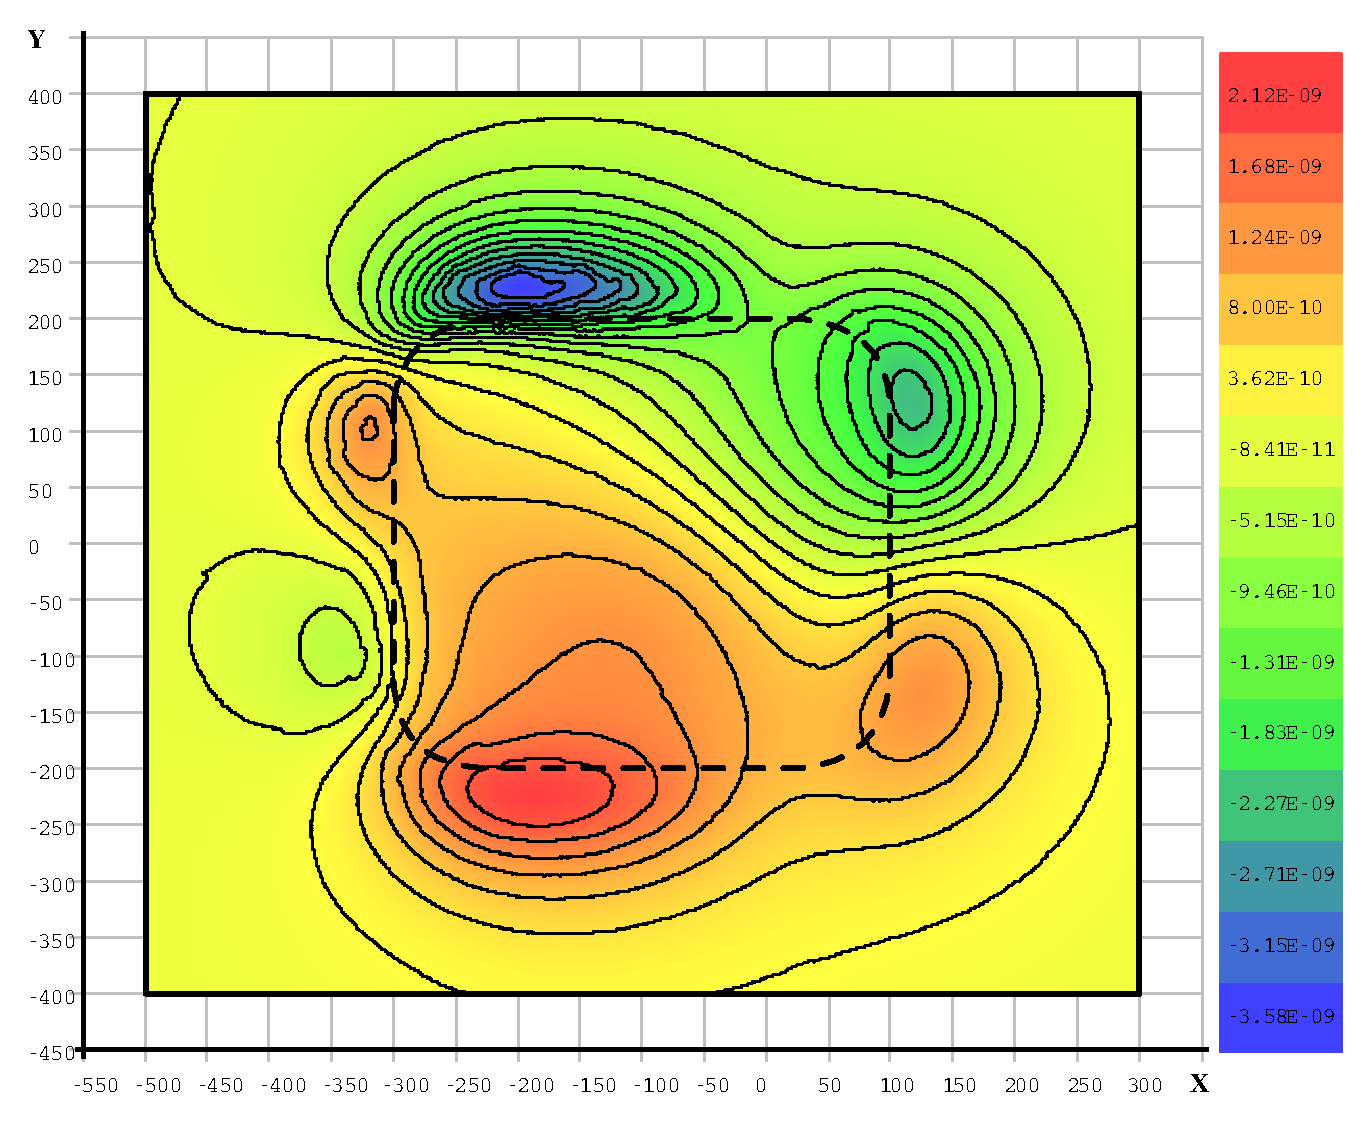
\includegraphics[scale=0.35]{research-3/fields/images/100/100_no_z=-601_EzR.eps}\label{fig:res3:100_EzR_a}}
	\text{~~}
	\subfloat[][]{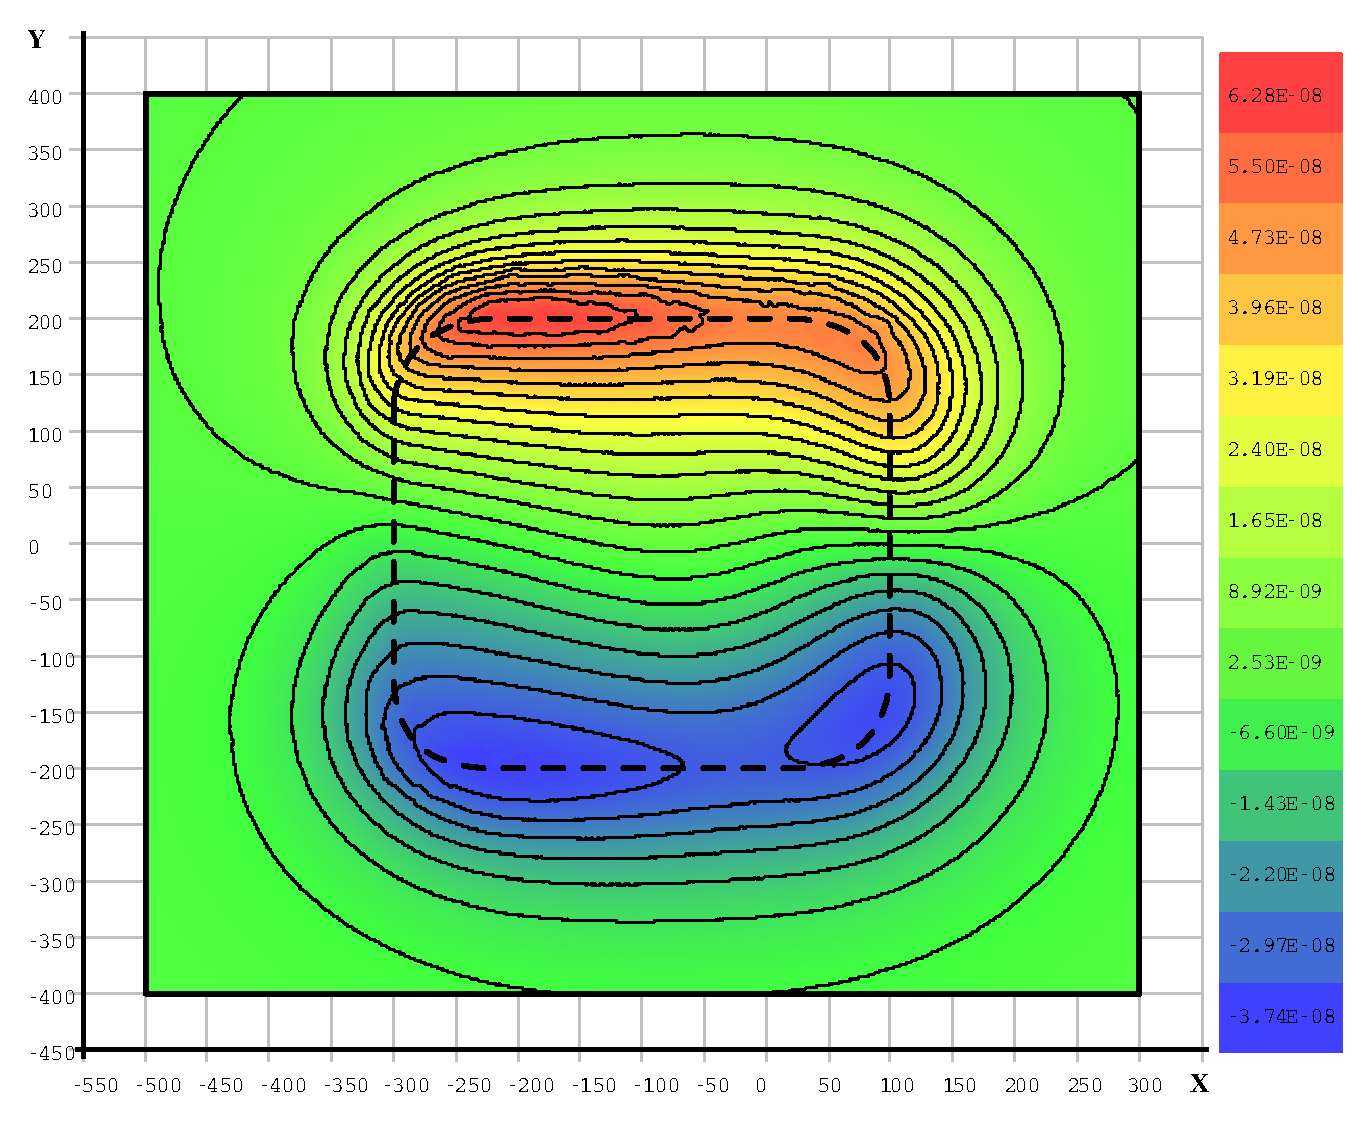
\includegraphics[scale=0.35]{research-3/fields/images/100/100_yes_z=-601_EzR.eps}\label{fig:res3:100_EzR_b}}
	\caption{$\Re(\mathbf{E}_z)$ при $l_2=-100$ в сечении $z=-601$}
	\label{fig:res3:100_EzR}
\end{figure}

\vspace{-0.8cm}

\begin{figure}[H]
	\centering
	\subfloat[][]{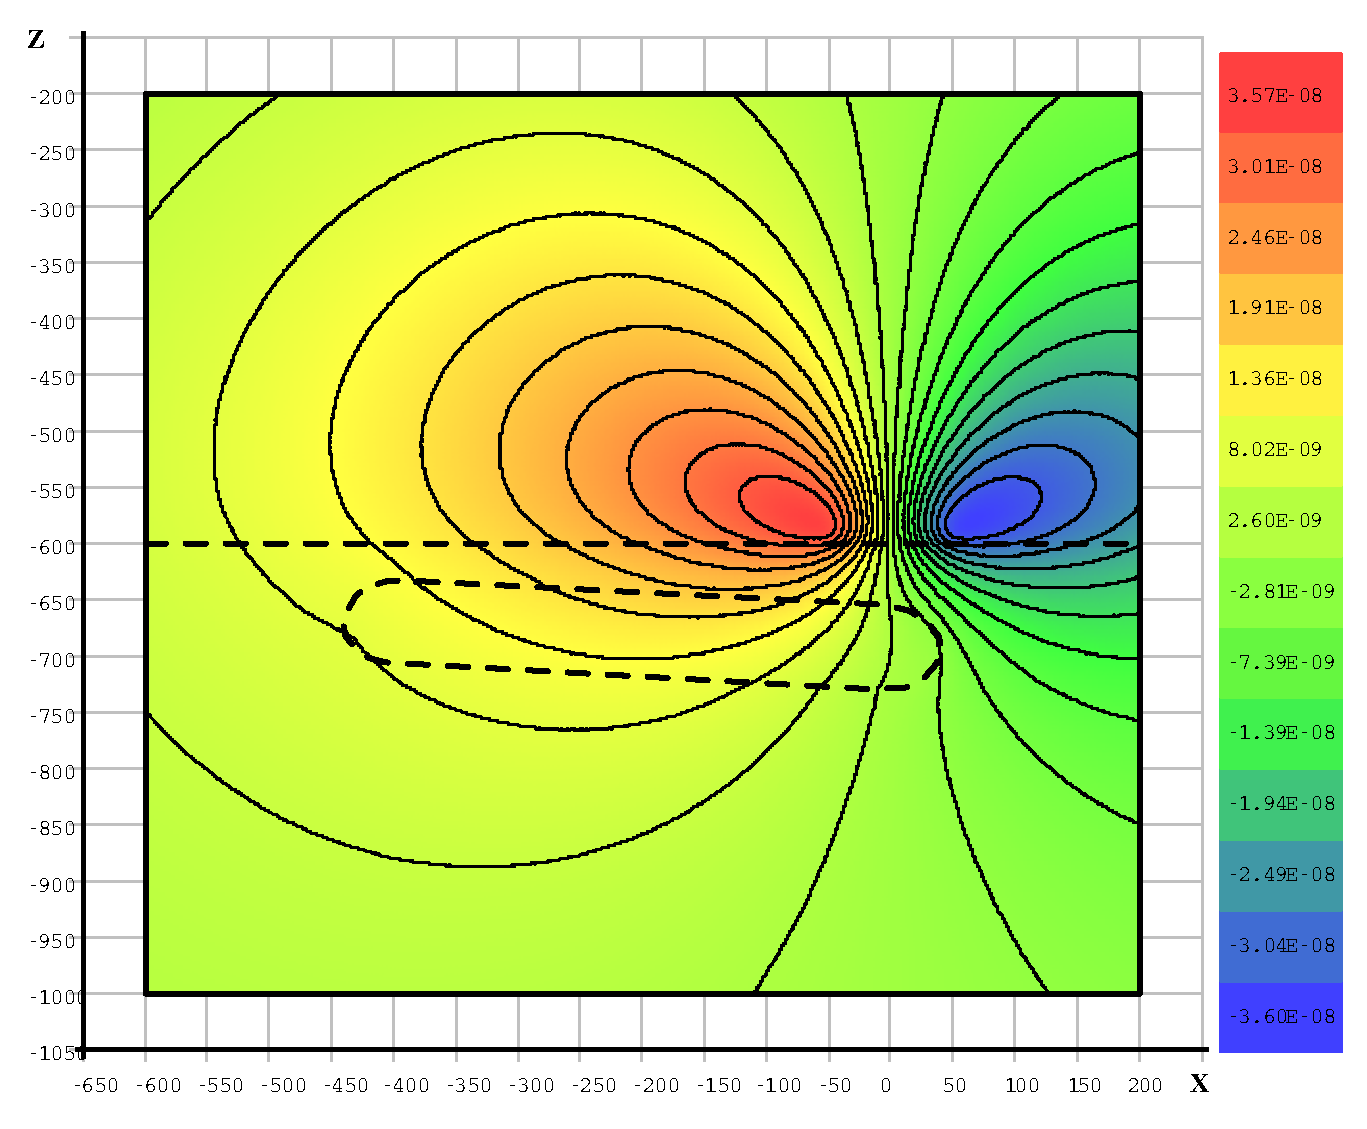
\includegraphics[scale=0.35]{research-3/fields/images/200/200_no_y=0_EyR.eps}\label{fig:res3:200_EyR_a}}
	\text{~~}
	\subfloat[][]{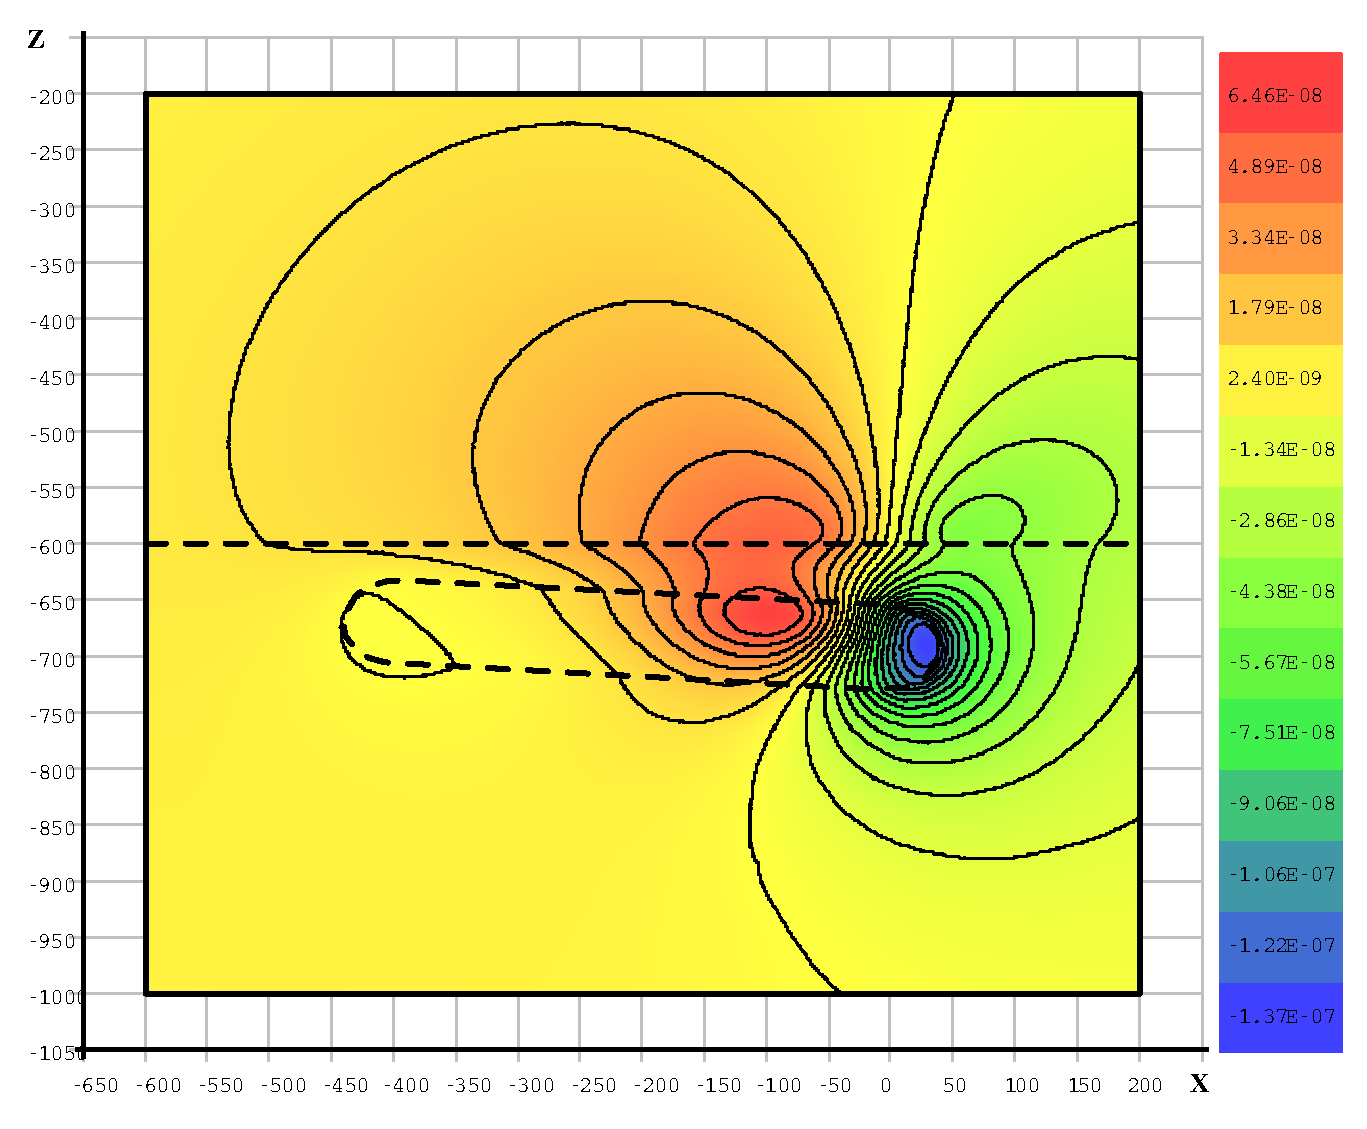
\includegraphics[scale=0.35]{research-3/fields/images/200/200_yes_y=0_EyR.eps}\label{fig:res3:200_EyR_b}}
	\caption{$\Re(\mathbf{E}_y)$ при $l_2=-200$ в сечении $y=0$}
	\label{fig:res3:200_EyR}
\end{figure}

\vspace{-0.8cm}

\begin{figure}[H]
	\centering
	\subfloat[][]{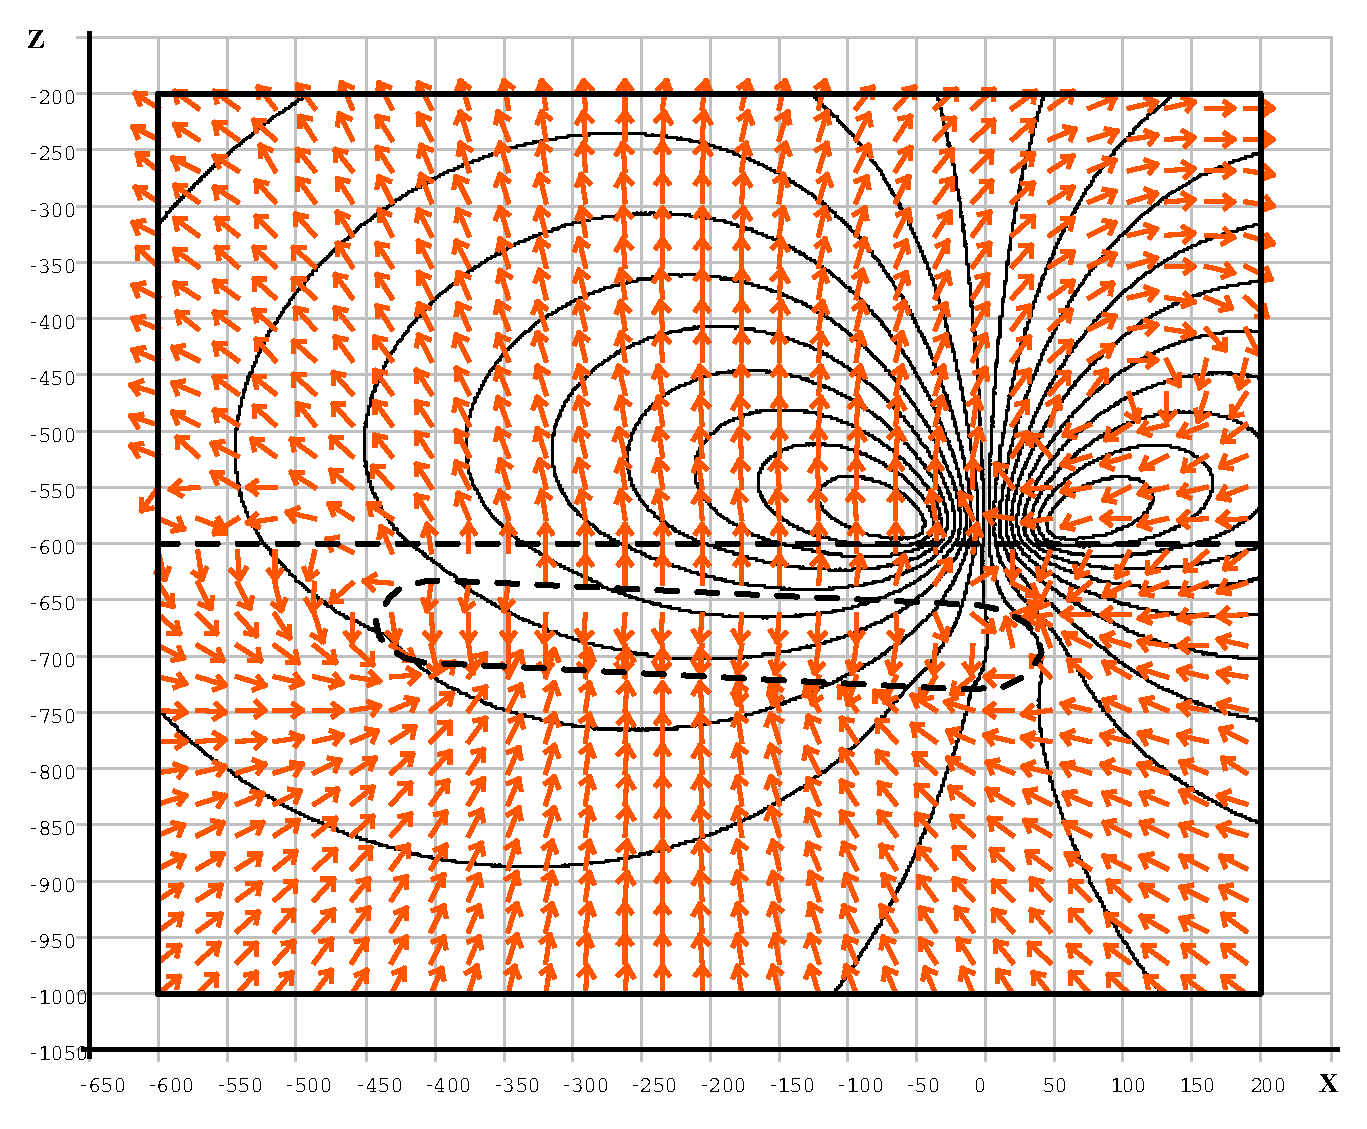
\includegraphics[scale=0.35]{research-3/fields/images/200/200_no_y=0_vec.eps}\label{fig:res3:200_vec_a}}
	\text{~~}
	\subfloat[][]{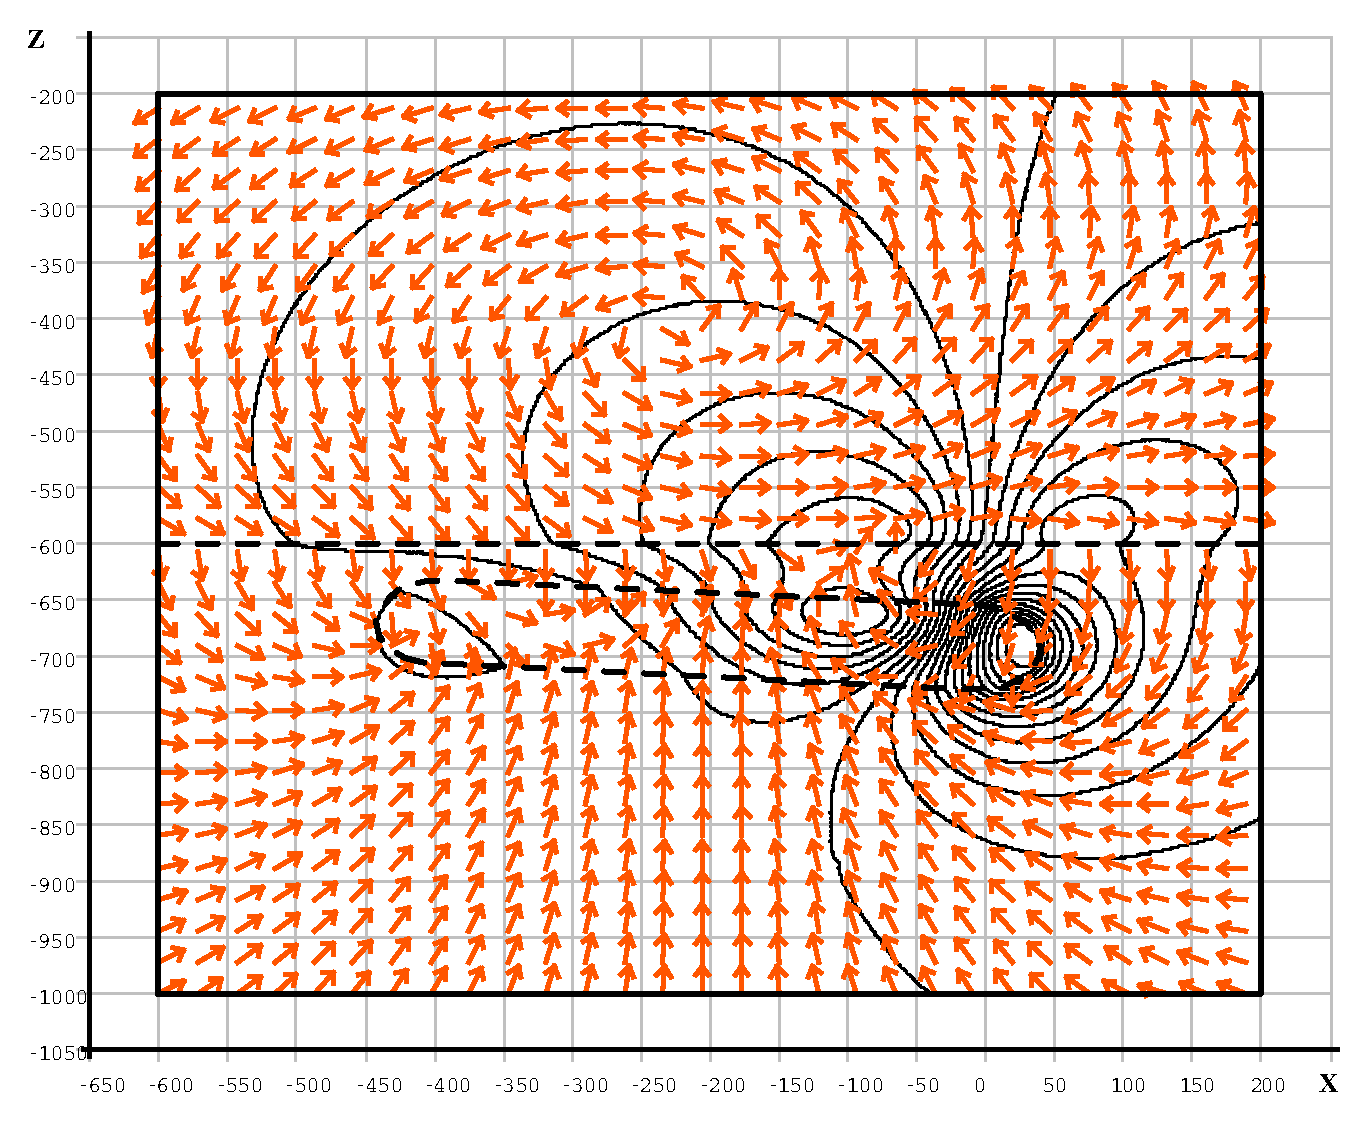
\includegraphics[scale=0.35]{research-3/fields/images/200/200_yes_y=0_vec.eps}\label{fig:res3:200_vec_b}}
	\caption{векторы $(\Re(\mathbf{E}_x), \Re{\mathbf{E}_z})^T$, изолинии $\Re(\mathbf{E}_y)$ при $l_2=-200$ в сечении $y=0$}
	\label{fig:res3:200_vec}
\end{figure}

\vspace{-0.8cm}

\begin{figure}[H]
	\centering
	\subfloat[][]{\includegraphics[scale=0.35]{research-3/fields/images/200/200_no_z=-601_EzR.eps}\label{fig:res3:200_EzR_a}}
	\text{~~}
	\subfloat[][]{\includegraphics[scale=0.35]{research-3/fields/images/200/200_yes_z=-601_EzR.eps}\label{fig:res3:200_EzR_b}}
	\caption{$\Re(\mathbf{E}_z)$ при $l_2=-200$ в сечении $z=-601$}
	\label{fig:res3:200_EzR}
\end{figure}

\vspace{-0.8cm}

\begin{figure}[H]
	\centering
	\subfloat[][]{\includegraphics[scale=0.35]{research-3/fields/images/300/300_no_y=0_EyR.eps}\label{fig:res3:300_EyR_a}}
	\text{~~}
	\subfloat[][]{\includegraphics[scale=0.35]{research-3/fields/images/300/300_yes_y=0_EyR.eps}\label{fig:res3:300_EyR_b}}
	\caption{$\Re(\mathbf{E}_y)$ при $l_2=-300$ в сечении $y=0$}
	\label{fig:res3:300_EyR}
\end{figure}

\vspace{-0.8cm}

\begin{figure}[H]
	\centering
	\subfloat[][]{\includegraphics[scale=0.35]{research-3/fields/images/300/300_no_y=0_vec.eps}\label{fig:res3:300_vec_a}}
	\text{~~}
	\subfloat[][]{\includegraphics[scale=0.35]{research-3/fields/images/300/300_yes_y=0_vec.eps}\label{fig:res3:300_vec_b}}
	\caption{векторы $(\Re(\mathbf{E}_x), \Re{\mathbf{E}_z})^T$, изолинии $\Re(\mathbf{E}_y)$ при $l_2=-300$ в сечении $y=0$}
	\label{fig:res3:300_vec}
\end{figure}

\vspace{-0.8cm}

\begin{figure}[H]
	\centering
	\subfloat[][]{\includegraphics[scale=0.35]{research-3/fields/images/300/300_no_z=-601_EzR.eps}\label{fig:res3:300_EzR_a}}
	\text{~~}
	\subfloat[][]{\includegraphics[scale=0.35]{research-3/fields/images/300/300_yes_z=-601_EzR.eps}\label{fig:res3:300_EzR_b}}
	\caption{$\Re(\mathbf{E}_z)$ при $l_2=-300$ в сечении $z=-601$}
	\label{fig:res3:300_EzR}
\end{figure}

\end{spacing}


Результаты моделирования показывают, что проводящий объект хорошо <<виден>> и на некотором расстоянии от морского дна, а непроводящий -- только вблизи поверхности или при некотором заглублении приемника в грунт, причем наибольший отклик на источник электромагнитного возмущения для непроводящего объекта наблюдается в том случае, когда этот источник расположен с некоторым смещением от центра симметрии объекта.

% =============================================================================

%\clearpage
\section{Описание программного комплекса}
%TODO Описать программный комплекс
{\color{red}\textbf{Описать программный комплекс}}

% =============================================================================

%\clearpage
\phantomsection
\section*{Заключение}
\addcontentsline{toc}{section}{Заключение}
%TODO Написать заключение
{\color{red}\textbf{Написать заключение}}

% =============================================================================

\clearpage
\addcontentsline{toc}{section}{Список литературы}

\begin{spacing}{1.2}

\begin{thebibliography}{10}
% 1
\bibitem{shurina} 
Шурина, Э.П. Морская геоэлектрика -- задачи и перспективы / Э.П. Шурина, М.И. Эпов, А.В. Мариенко // Тезисы докладов всероссийской научно-технической конференции "Научное и техническое обеспечение исследования и освоения шельфа Северного Ледовитого океана". -- 2010. -- 9-13~августа. -- С.~7-12.
% 2
\bibitem{gabrielsen} 
Gabrielsen, P.T. 3D CSEM for Hydrocarbon Exploration in the Barents Sea / P.T. Gabrielsen, D.V. Shantsev, S. Fanavoll // 5th Saint Petersburg International Conference \& Exhibition -- Geosciences: Making the most of the Earth’s resources. -- 2012. -- 2-5~April. -- P.~1-5.
% 3
\bibitem{berenger}
Berenger, J.P. A perfectly matched layer for the absorption of electromagnetic waves / J.P. Berenger // Jurnal of computation physics 114, 185-200, 1994
% 4
\bibitem{wiik_dehoop_ursin}
Wiik, T. A Discontinuous Galerkin Method for Modelling Marine Controlled Source Electromagnetic Data / T. Wiik, M.V. De Hoop, B. Ursin // Proceedings of the Project Review, Geo-Mathematical Imaging Group, Purdue University, West Lafayette, IN, Vol. 1 (2013) pp. 75-102.
% 5
\bibitem{epov}
Эпов, М.И. Параллельные конечноэлементные вычислительные схемы в задачах геоэлектрики / М.И. Эпов, Э.П. Шурина, Д.А. Архипов // Вычислительные технологии. -- 2013. -- Том~18, №2. -- С.~94-112.
% 6
\bibitem{balandin} 
Баландин, М.Ю. Векторный метод конечных элементов : Учеб. пособие / М.Ю. Баландин, Э.П. Шурина. -- Новосибирск : Изд-во НГТУ, 2001. -- 69~с.
% 7
\bibitem{webb1999}
Webb, J.P. Hierarchal Vector Basis Functions of Arbitrary Order for Triangular and Tetrahedral Finite Elements / J.P. Webb // IEEE transactions on antennas and propagation. -- 1999. -- Vol.~47. -- P.~1244-1253.
% 8
\bibitem{nechaev}
Nechaev, O.V. Multilevel iterative solver for the edge fem solution of the 3D Maxwell equation / O.V. Nechaev, E.P Shurina, M.A. Botchev // Computers and Mathematics with Applications. -- 2008. -- №55. -- P.~2346-2362.
% 9
\bibitem{soloveychick}
Соловейчик, Ю.Г. Метод конечных элементов для решения скалярных и векторных задач : учеб. пособие / Ю.Г. Соловейчик, М.Э. Рояк, М.Г. Персова. -- Новосибирск : Изд-во НГТУ, 2007. -- 896~с.

\bibitem{monk}
Monk P. Finite element methods for Maxwell's equations. -- Oxford University Press, 2003.
\bibitem{schwarzbach}
Schwarzbach C. Stability of finite element solutions to Maxwell's equations in frequency domain. -- 2009.
\bibitem{hiptmair}
Hiptmair R. Multigrid method for Maxwell's equations // SIAM Journal on Numerical Analysis. -- 1998. -- Т. 36. -- №. 1. -- С. 204-225.
\bibitem{nedelec1980}
Nédélec J. C. Mixed finite elements in $\mathbb{R}$3 //Numerische Mathematik. -- 1980. -- Т. 35. -- №. 3. -- С. 315-341.
\bibitem{nedelec1986}
Nédélec J. C. A new family of mixed finite elements in $\mathbb{R}$3 //Numerische Mathematik. -- 1986. -- Т. 50. -- №. 1. -- С. 57-81.
\bibitem{webb1993}
Webb J. P. Edge elements and what they can do for you //Magnetics, IEEE Transactions on. -- 1993. -- Т. 29. -- №. 2. -- С. 1460-1465.
\bibitem{mikhajlova}
Михайлова Е. И., Шурина Э. П. Математическое моделирование высокочастотного электромагнитного поля в волноводных устройствах //Вестник НГУ. Серия: Математика, механика, информатика. -- 2013. -- Т. 13. -- №. 4. -- С. 102-118.
\bibitem{misovskih}
Мысовских И. П. Интерполяционные кубатурные формулы. -- Наука. Гл. ред. физ.-мат. лит., 1981.
\bibitem{zhang_integration}
Zhang L. et al. A set of symmetric quadrature rules on triangles and tetrahedra //J. Comput. Math. -- 2009. -- Т. 27. -- №. 1. -- С. 89-96.
\bibitem{tet_integration}
Numerical Integration over the Tetrahedral Domain [Электронный ресурс].
-- Режим доступа: \href{https://web.archive.org/web/20140714140951/https://people.fh-landshut.de/~maurer/numeth/node148.html}{\url{https://people.fh-landshut.de/~maurer/numeth/node148.html}}.
\bibitem{tr_integration}
Numerical Integration over the Triangular Domain [Электронный ресурс].
-- Режим доступа: \href{https://web.archive.org/web/20140714120045/https://people.fh-landshut.de/~maurer/numeth/node147.html}{\url{https://people.fh-landshut.de/~maurer/numeth/node147.html}}.
\bibitem{anderson}
Anderson C. An integrated approach to marine electromagnetic surveying using a towed streamer and source / Anderson C., Mattsson J. // First Break. -- May 2010. -- Volume 28, Issue 5. -- P. 71-75.
\bibitem{mur}
Mur G. Absorbing boundary conditions for the finite-difference approximation of the time-domain electromagnetic-field equations //Electromagnetic Compatibility, IEEE Transactions on. -- 1981. -- №. 4. -- С. 377-382.
\end{thebibliography}

\end{spacing}

% =============================================================================

\end{document}
